\documentclass[12pt,twoside,book]{article}
\usepackage{docmute}

\input{settings}

\graphicspath{{./Model/}{./DM/}{./Direct/}{./Drell-Yan/}{./SUSY/}{./DY-Appendix/}}

\begin{document}

\begin{titlepage}

\begin{center}

\begin{titlelineskip}

\vskip .75in

{\Large \it

 Ph.D. Thesis

}

\vskip 1.0in

{\Huge \bf

  Probing Electroweakly Interacting\\
  Massive Particles\\
  with Drell-Yan Process\\
  at 100 TeV Colliders

}

\vskip .75in

{\Large
So Chigusa
}\\

{\Large \it Department of Physics}

\vfill

\centering

\includegraphics[width=0.6\hsize]{univ.eps}

\vskip 0.35in

{\Large December 2019}

\end{titlelineskip}

\end{center}

\vspace{0.5in}

\end{titlepage}

\thispagestyle{empty}

\vspace*{1.50in}

\begin{abstract}
 \rem{To be written}
\end{abstract}

\clearpage

\thispagestyle{empty}

\vspace*{.75in}

{\LARGE \bf
Acknowledgments
}

\vskip .50in

\rem{To be written}

% I would like to thank my supervisor, Takeo Moroi, who provided
% stimulating discussions, helpful comments, fruitful suggestions and
% collaboration.  I am also grateful to Koichi Hamaguchi, Kazunori
% Nakayama, Natsumi Nagata and all the members of the particle physics
% group at the University of Tokyo for their hospitality.  My work is
% supported by the Program for Leading Graduate Schools, MEXT, Japan.
% Finally, I would like to express my gratitude to my family, friends and
% all things which allow me to enjoy studying physics.

\clearpage

\thispagestyle{empty}

\tableofcontents

\clearpage

\renewcommand{\thepage}{\arabic{page}}
\setcounter{page}{1}

%%%%%%%%%%%%%%%%%%%%%%%%%%%%%%%%%%%%%%%%%%%%%%%%%%%%%%%%%%%%%%%%%%%%%%%%%%%%%%%
\section[Introduction]{Introduction}
\setcounter{equation}{0}
%%%%%%%%%%%%%%%%%%%%%%%%%%%%%%%%%%%%%%%%%%%%%%%%%%%%%%%%%%%%%%%%%%%%%%%%%%%%%%%

\vskip 0.1in

\rem{Unit: $\hbar=c=k_B=1$ and definition of $g_1$ and etc?}

\rem{Definition of Feynmann Slash (Exception: missing transverse momentum)}

\rem{Definition of $\sigma$ matrices}

\rem{Convention: dot as time derivative}

\rem{Definition of ``SM''}

\rem{Definition of ``WIMP''}

\rem{Definition of ``DM''}

\rem{Normalization of $g_1$?}

\footnote{
  Some authors use the word ``WIMPs'' in a broad sence to mention some particles that have interactions with others whose size is comparable to the electroweak gauge coupling.
  To distinguish this usage with ours, which only denotes some particles with non-zero electroweak charge, it may be better to call them as ``Electroweakly Interacting Massive Particles (EWIMPs)''.
  However, within this thesis, we will just use ``WIMPs'' in a narrow sence obeying the widely spread custom.
}

The rest of the paper is organized as follows.

\clearpage

% Erase biblio in input file before turning on
\documentclass[12pt,twoside,book]{article}
\usepackage{docmute}

\input{../settings}

\begin{document}

%%%%%%%%%%%%%%%%%%%%%%%%%%%%%%%%%%%%%%%%%%%%%%%%%%%%%%%%%%%%%%%%%%%%%%%%%%%%%%%
\section{Models with WIMPs}
\setcounter{equation}{0}
%%%%%%%%%%%%%%%%%%%%%%%%%%%%%%%%%%%%%%%%%%%%%%%%%%%%%%%%%%%%%%%%%%%%%%%%%%%%%%%

\vskip 0.1in

There are several examples of the models that contain WIMP DM
candidates.  In this section, two of them \rem{Really?} are briefly
reviewed.  \rem{EWIMP and WIMP??}

%%%%%%%%%%%%%%%%%%%%%%%%%%%%%%%%%%%%%%%%%%%%%%%%%%%%%%%%%%%%%%%%%%%%%%%%%%%%%%%
\subsection{Minimally supersymmetric standard model}
%%%%%%%%%%%%%%%%%%%%%%%%%%%%%%%%%%%%%%%%%%%%%%%%%%%%%%%%%%%%%%%%%%%%%%%%%%%%%%%

\rem{Summary of SUSY particle names somewhere}

\begin{figure}[b]
  \centering
  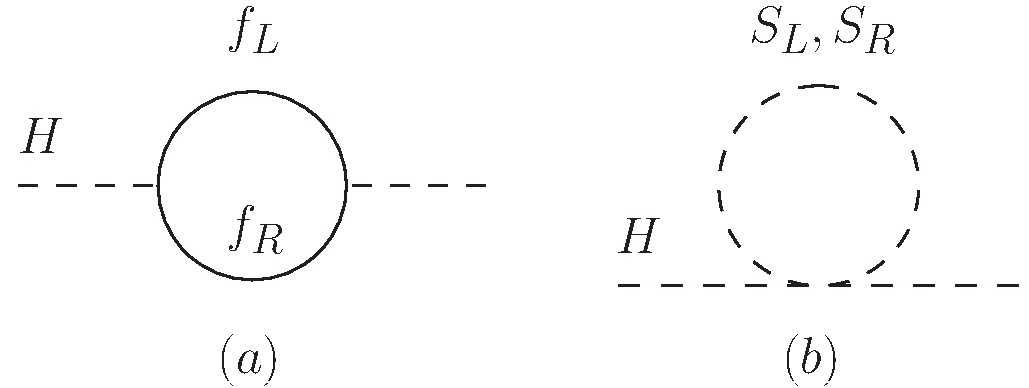
\includegraphics[width=0.6\hsize]{loop_correction.pdf}
  \caption{One-loop correction to the Higgs mass from (a) a Weyl fermion $f$ and (b) a complex scalar $S$.}
  \label{fig:loop_correction}
\end{figure}

The minimally supersymmetric standard model (MSSM) is the simple extension of the SM with $\mathcal{N} = 1$ supersymmetry (SUSY).
\footnote{
  For a brief review of the $\mathcal{N} = 1$ SUSY, see Sec.~\ref{sec:susy}.
}
One of the motivations to introduce SUSY is to solve the so-called hierarchy (or naturalness) problem \cite{Weinberg:1975gm,Gildener:1976ai,Susskind:1978ms} in the SM.
The problem is related to the quantum correction to the SM Higgs boson mass from heavy new physics particles.
For example, we can consider the one-loop correction to the Higgs mass from a Weyl fermion $f$ and a complex scalar $S$ as illustrated in Fig.~\ref{fig:loop_correction}.
The corrections to the Higgs mass is given by
\begin{align}
  \Delta m_h^2 &= -\frac{|\lambda_f|^2}{8 \pi^2} \left[
  \Lambda_{\mathrm{UV}}^2 - 2 m_f^2 \ln \left( \frac{\Lambda_{\mathrm{UV}}}{m_f} \right)
  + \cdots \right] & &\mathrm{(fermion)}, \label{eq:delmh_f}\\
  \Delta m_h^2 &= \frac{\lambda_S}{16 \pi^2} \left[
  \Lambda_{\mathrm{UV}}^2 - 2 m_S^2 \ln \left( \frac{\Lambda_{\mathrm{UV}}}{m_S} \right)
  + \cdots \right] & &\mathrm{(scalar)}, \label{eq:delmh_S}
\end{align}
\rem{Check this!}
where $\lambda_f$ and $m_f$ are the Higgs-fermion coupling constant and the fermion mass, respectively, and $\lambda_S$ and $m_S$ are those for the scalar $S$.
We take the cut-off scale of the theory to be $\Lambda_{\mathrm{UV}}$ to regularize the otherwise divergent loop integral and neglect the lower order terms of $\Lambda_{\mathrm{UV}}$.
Eqs.~\eqref{eq:delmh_f} and \eqref{eq:delmh_S} show the quadratic dependence of $\Delta m_H^2$ on $\Lambda_{\mathrm{UV}}$, which means that the Higgs mass is sensitive to the energy scale of the beyond the SM physics.
However, there is at least one extremelly high energy scale physics in the nature, gravity at the Planck scale $M_{\mathrm{pl}} \sim 10^{18 \hyphen 19}\,\mathrm{GeV}$.
By substituting $\Lambda_{\mathrm{UV}} = M_{\mathrm{pl}}$ in Eqs.~\eqref{eq:delmh_f} and \eqref{eq:delmh_S} and assuming $\lambda_f \sim \lambda_S \sim \mathcal{O} (1)$, we notice that orders-of-magnitude fine-tuning is required to obtain the correct Higgs mass $m_h = 125.10\,\mathrm{GeV}$ \cite{Tanabashi:2018oca}, which is unnatural.

SUSY provides a nice solution to this fine-tuning problem.
As is summarized in Appendix~\ref{sec:susy}, \rem{summarize later} each Weyl fermion in a supersymmetric model has two complex scalars with the same mass $m_f = m_S$.
In addition, their coupling constants should have a relationship $|\lambda_f|^2 = \lambda_S$ due to the fact that $\lambda_S$ is a coupling constant in the F-term potential sourced by a superpotential term proportional to $\lambda_f$. \rem{description of F-term and D-term}
By using both equations and summing the corrections \eqref{eq:delmh_f} and \eqref{eq:delmh_S} with factor of two multiplied to the latter, we obtain a result independent of the cut-off scale $\Lambda_{\mathrm{UV}}$ without fine-tuning.
This cancellation is ensured by the so-called non-renormalization theorem. \cite{Salam:1974jj, Grisaru:1979wc}

\begin{table}[t]
  \centering
  \begin{tabular}{c|ccc}
    Notation & $SU(3)_C$ & $SU(2)_L$ & $U(1)_Y$ \\ \hline
    $\hat{Q}_i$ & $\bm{3}$ & $\bm{2}$ & $1/6$ \\
    $\hat{L}_i$ & $\bm{1}$ & $\bm{2}$ & $-1/2$ \\
    $\hat{U}_i$ & $\bar{\bm{3}}$ & $\bm{1}$ & $-2/3$ \\
    $\hat{D}_i$ & $\bar{\bm{3}}$ & $\bm{1}$ & $1/3$ \\
    $\hat{E}_i$ & $\bm{1}$ & $\bm{1}$ & $1$ \\
    $\hat{H}_u$ & $\bm{1}$ & $\bm{2}$ & $1/2$ \\
    $\hat{H}_d$ & $\bm{1}$ & $\bm{2}$ & $-1/2$
  \end{tabular}
  \caption{Notations and quantum numbers of the chiral superfields in the MSSM.}
  \label{tab:mssm_csf}
\end{table}

\begin{table}[t]
  \centering
  \begin{tabular}{c|ccc}
    Notation & $SU(3)_C$ & $SU(2)_L$ & $U(1)_Y$ \\ \hline
    $\hat{g}$ & $\bm{8}$ & $\bm{1}$ & $0$ \\
    $\hat{W}$ & $\bm{1}$ & $\bm{3}$ & $0$ \\
    $\hat{B}$ & $\bm{1}$ & $\bm{1}$ & $0$ \\
  \end{tabular}
  \caption{Notations and quantum numbers of the vector superfields in the MSSM.}
  \label{tab:mssm_vsf}
\end{table}

We now summarize the notations and quantum numbers of the chiral and vector superfields in the MSSM in Table~\ref{tab:mssm_csf} and \ref{tab:mssm_vsf}, respectively.
The supersymmetric part of the MSSM lagrangian is described by the superpotential
\footnote{
  For a more detailed review of the MSSM, see for example~\cite{Martin:1997ns}.
}
\begin{align}
  W = Y_u^{i j} \hat{U}_i \hat{Q}_j \hat{H}_u - Y_d^{i j} \hat{D}_i \hat{Q}_j \hat{H}_d
  - Y_e^{i j} \hat{E}_i \hat{L}_j \hat{H}_d + \mu \hat{H}_u \hat{H}_d,
  \label{eq:mssm_sup}
\end{align}
where $i,j=1,2,3$ labels the quark and lepton generation, while $Q, L, U, D, E$ are superfields that contain the left-handed quark, left-handed lepton, right-handed up-type quark, right-handed down-type quark, and right-handed charged lepton, respectively.
In Eq.~\eqref{eq:mssm_sup}, proper contraction of $SU(3)_C$ and $SU(2)_L$ indices is assumed.
Note that two Higgs doublets $H_u$ and $H_d$ with opposite values of $U(1)_Y$ hypercharges are introduced, which is needed to cancel the contributions to the gauge anomaly from fermionic partners of the Higgs doublets.

Postulating SM gauge symmetries as a unique guideline to construct a model, there are a few more terms allowed in the superpotential:
\begin{align}
  W_{\Delta L=1} &= \lambda^{ijk} \hat{L}_i \hat{L}_j \hat{E}_k + \lambda^{'ijk} \hat{L}_i \hat{Q}_j \hat{D}_k
  + \mu^i \hat{L}_i \hat{H}_u, \label{eq:super_L} \\
  W_{\Delta B=1} &= \lambda^{''ijk} \hat{U}_i \hat{D}_j \hat{D}_k. \label{eq:super_B}
\end{align}
Terms in Eqs.~\eqref{eq:super_L} and \eqref{eq:super_B} are phenomenologically problematic since they lead to the lepton and baryon number violating operators, respectively, which may cause a too fast proton decay, depending on parameters (see for example \cite{Sakai:1981pk}).
To avoid this problem, we often rely on a symmetry called the R-parity \cite{Farrar:1978xj} or the matter parity \cite{Dimopoulos:1981zb, Weinberg:1981wj, Sakai:1981pk, Dimopoulos:1981yj}.
Charges of the R-parity, which is basically a $Z_2$ symmetry, are calculated as
\begin{align}
  P_R = (-1)^{3(B-L)+2s},
\end{align}
where $B$, $L$, and $s$ are the baryon number, lepton number, and spin of the particle, respectively.
According to the definition, we can see that all the SM particles have even parity ($P_R = +1$), while all the supersymmetric particles have odd parity ($P_R = -1$).
Then it is easy to check that Eqs.\eqref{eq:super_L} and \eqref{eq:super_B} lead to the R-parity violating terms in the Lagrangian and thus are forbidden, while all the terms in Eq.~\eqref{eq:mssm_sup} remain allowed.
From now on, we only focus on the R-parity conserving MSSM.

Since no superpartner of any SM particle is observed yet, SUSY should be broken and superpartners should obtain the SUSY breaking masses.  \rem{ref: boson and fermion obtain equal mass}
The SUSY breaking part of the lagrangian is expressed as
\begin{align}
  \mathcal{L}_{\mathrm{soft}} =&
  -\frac{1}{2} \left( M_3 \g \g + M_2 \W \W + M_1 \B \B + \mathrm{c.c.} \right) \notag \\&
  -\left( A_u^{ij} \U_i \Q_j H_u - A_d^{ij} \D_i \Q_j H_d - A_e^{ij} \E_i \L_j H_d \right) \notag \\&
  -m_Q^{2ij} \Q^\dagger_i \Q_j - m_L^{2ij} \L^\dagger_i \L_j - m_U^{2ij} \U^\dagger_i \U_j
  -m_D^{2ij} \D^\dagger_i \D_j - m_E^{2ij} \E^\dagger_i \E_j \notag \\&
  -m_{H_u}^2 H_u^{*} H_u - m_{H_d}^2 H_d^{*} H_d - \left( b H_u H_d + \mathrm{c.c.} \right),
  \label{eq:mssm_soft}
\end{align}
where the tilde is used to express the superpartner of the SM particle contained in a superfield, while a field without a hat nor tilde denotes the other component.
An exception is two Higgs doublets, where $H_u$ and $H_d$ express the scalar components, while $\tilde{H}_u$ and $\tilde{H}_d$ express their superpartners called Higgsinos.
The SM-like Higgs doublet $H$ collesponds to a linear combination of $H_u$ and $H_d$.

It is known that, within the MSSM, almost all SUSY breaking mechanisms, such as the F-term (O$^{\mathrm{\prime}}$Raifeartaigh) \cite{ORaifeartaigh:1975nky} or D-term (Fayet-Iliopoulos) SUSY breaking \cite{Fayet:1974jb, Fayet:1974pd}, fail to generate masses of superpartners with remaining the SM gauge group in the low energy effective theory.
Thus, we need a so-called hidden sector in addition to the MSSM sector, in which SUSY is spontaneously broken.
In order for the MSSM sector to have Lagrangian terms \eqref{eq:mssm_soft}, we also need some mediation mechanism of the SUSY breaking.
The relative size of the SUSY breaking parameters in Eq.~\eqref{eq:mssm_soft} highly depends on the mediation mechanism.
Among many mediation mechanisms of SUSY breaking, the anomaly mediated SUSY breaking \cite{Giudice:1998xp, Randall:1998uk} leads to an interesting phenomenology with relatively light WIMPs, so it will be reviewed later.


\subsubsection*{Dark matter candidate in the MSSM}

There is another motivation to consider the (R-parity preserving) MSSM: the existence of the DM.
Since there is a sizable amount of DM in the current universe, a DM candidate should be stable or have sufficiently small decay width.
In many models, the stability of DM is ensured by imposing a symmetry and/or by kinematically forbidding the DM decay.
In the MSSM, the role of stabilizer can be played by the R-symmetry described above.
Recalling that all the SM (supersymmetric) particles have even (odd) parity, each interaction vertex in the MSSM Lagrangian should contain an even number of supersymmetric particles.
If we consider the lightest supersymmetric particle (LSP), such vertices can not construct the kinematically allowed LSP decay chain and, as a result, the LSP becomes a stable DM candidate.

The DM phenomenology, such as the production and annihilation of DM in the universe and processes that allow us to efficiently detect it, highly depends on which species of supersymmetric particle becomes the LSP.
Hereafter, we only focus on the cases where one of the gauginos and Higgsinos becomes the LSP with some motivations described below.
In addition, all the LSP candidates to be described have non-zero electroweak charges and they can be viewed as examples of the WIMPs.


\subsubsection*{Higgs mass in the MSSM}

Under the spontaneously broken SUSY, the cancellation of the quantum correction to the Higgs boson discussed above is not exact.
One obvious consequence of the SUSY breaking in Eqs.~\eqref{eq:delmh_f} and \eqref{eq:delmh_S} is the hierarchy between $m_f$ and $m_S$ that appear in the second term of each contribution.
In the case of the MSSM, the largest contribution comes from the superpartner of the top quark, stop, that have the largest Yukawa coupling with the Higgs boson.

\begin{table}[t]
  \centering
  \begin{tabular}{ccc}
    Value & Description & Reference\\ \hline
    $M_W = 80.384 \pm 0.014\, \mathrm{GeV}$ & Pole mass of the W boson
      & \cite{Group:2012gb,Alcaraz:1016509} \\
    $M_Z = 91.1876 \pm 0.0021\, \mathrm{GeV}$ & Pole mass of the Z boson
      & \cite{Beringer:1900zz} \\
    $M_h = 125.15 \pm 0.24\, \mathrm{GeV}$ & Pole mass of the Higgs
      & \cite{Aad:2013wqa,Chatrchyan:2013mxa} \\
    $M_t = 173.34 \pm 0.82\, \mathrm{GeV}$ & Pole mass of the top quark
      & \cite{ATLAS:2014wva} \\
    $\left( \sqrt{2} G_\mu \right)^{-1/2} = 246.21971 \pm 0.00006\, \mathrm{GeV}$
      & Fermi constant for $\mu$ decay & \cite{Tishchenko:2012ie} \\
    $\alpha_3 (M_Z) = 0.1184 \pm 0.0007$
      & $\overline{\mathrm{MS}}$ $SU(3)_C$ gauge coupling & \cite{Bethke:2012jm}
  \end{tabular}
  \caption{Experimentally measured SM parameters used for the derivation of Eq.~\eqref{eq:lambda_at_top}.}
  \label{tab:SM_param}
\end{table}

When there is a large hierarchy between the SUSY breaking scale $M_S$, which is comparable with stop masses, and the top mass $M_t$, the stop contributions to the Higgs mass contains a large logarithm of the form of $\log \left( M_S^2 / M_t^2 \right)$.
\rem{Consistency with above equations.  Maybe MSbar better}
To resum this large logarithm and obtain a precise result, we have to rely on the renormalization group equation (RGE).
In this framework, the value of the Higgs self coupling $\lambda$ at the electroweak scale is closely related to the Higgs mass.
We assume the SM parameters summarized in Table~\ref{tab:SM_param} and the definition of the SM Higgs potential
\begin{align}
  V(H) = -\frac{m^2}{2} |H|^2 + \lambda |H|^4,
\end{align}
with $H$ being the SM Higgs doublet.
Then, according to \cite{Buttazzo:2013uya}, we obtain the relationship
\footnote{
  Although the values listed in Table~\ref{tab:SM_param} are different from the latest ones given in \cite{Tanabashi:2018oca}, we use older ones because the change in input values may cause the slight change in coefficients of second and third terms of Eq.~\eqref{eq:lambda_at_top}.
  The latest central values of the Higgs and top masses are $M_h = 125.10\,\mathrm{GeV}$ and $M_t = 173.1\,\mathrm{GeV}$, with which we can estimate $\lambda (M_t) = 0.12595$.
}
\begin{align}
  \lambda (M_t) = 0.12604
  + 0.00206 \left( \frac{M_h}{\mathrm{GeV}} - 125.15 \right)
  - 0.00004 \left( \frac{M_t}{\mathrm{GeV}} - 173.34 \right),
  \label{eq:lambda_at_top}
\end{align}
where the $\overline{\mathrm{MS}}$ scheme is used to renormalize the divergence of loop integrals.

In the MSSM, the value of $\lambda$ at the SUSY breaking scale $M_S$ is given by
\begin{align}
  \lambda (M_S) = \frac{g_1^2 (M_S) + g_2^2 (M_S)}{8} \cos^2 2\beta + \delta \lambda,
  \label{eq:lambda_at_ms}
\end{align}
where $g_1$ and $g_2$ are $U(1)_Y$ and $SU(2)_L$ gauge coupling constants, respectively, while $\beta$ parametrizes the ratio of the vacuum expectation values
\begin{align}
  \frac{\Braket{H_u^0}}{\Braket{H_d^0}} = \tan \beta,
\end{align}
with $H_u^0$ and $H_d^0$ being electromagnetically neutral components of the corresponding Higgs doublets.
In Eq.~\eqref{eq:lambda_at_ms}, the first term shows the tree-level contribution from the D-term potential and $\delta \lambda$ denotes the threshold correction from heavy superpartners.
Once the spectrum of the MSSM particles is fixed, we can evaluate the Higgs self coupling using Eq.~\eqref{eq:lambda_at_ms}, calculate its running according to the RGE, and obtain the prediction for the Higgs mass through Eq.~\eqref{eq:lambda_at_top}.

\begin{figure}[t]
  \centering
  \includegraphics[width=0.6\hsize]{higgs_mass.pdf}
  \caption{
    Contour of the Higgs mass $m_h$ in the $\tan\beta$ vs. $M_S$ plane.
    The universal mass $M_S$ is assumed for all the SUSY particles.
    Blue (red) lines correspond from top to bottom to the contours of $m_h = 131, 128, 125, 122, 119\, \mathrm{GeV}$ for the minimal (maximal) stop mixing.
    Gray shade corresponds to the region where $m_h = 125.10\,\mathrm{GeV}$ can be explained.
  }
  \label{fig:higgs_mass}
\end{figure}

In Fig.~\ref{fig:higgs_mass}, we show the contour plot of the Higgs mass $m_h$ in the $\tan\beta$ vs. $M_S$ plane.
We assume the universal mass $M_S$ for all the SUSY particles.
Under this assumption, the largest contribution to the threshold correction $\delta \lambda$ from stops can be written as
\begin{align}
  \delta \lambda &\simeq \frac{9 y_t^2 (M_S)}{16 \pi^2} \tilde{X}_t \left[ 1-\frac{\tilde{X}_t}{12} \right], \label{eq:del_lambda}\\
  \tilde{X}_t &\equiv \frac{(A_t - \mu \cot \beta)^2}{M_S^2},
\end{align}
with $y_t \equiv Y_u^{33}$ and $A_t \equiv A_u^{33}$.
It is obvious from Eq.~\eqref{eq:del_lambda} that, for a moderate value of $\tilde{X}_t \lsim \mathcal{O}(1)$, $\tilde{X}_t = 0$ ($\tilde{X}_t = 6$) corresponds to the case with minimum (maximum) threshold correction, often called as the minimal (maximal) stop mixing.
\footnote{
  Eq.~\eqref{eq:del_lambda} shows that $\delta \lambda < 0$ for $\tilde{X}_t > 12$, resulting in the prediction of a lighter Higgs mass than the minimal stop mixing case.
  However, the parameter space with $\tilde{X}_t \gsim 6$ is severely constrained by the requirement of the stability of the electroweak vacuum \rem{Reference!!} and is not considered here.
}

The red (blue) lines in Fig.~\ref{fig:higgs_mass} denote from top to bottom the contours of $m_h = 131$, $128$, $125$, $122$, $119\, \mathrm{GeV}$ for the minimal (maximal) stop mixing.
Gray shade corresponds to the region where the central value of the observation $m_h = 125.10\,\mathrm{GeV}$ can be explained.
From the figure, we can see that the discovery of the Higgs with $m_h = 125.10\,\mathrm{GeV}$ may indicate a somewhat heavy SUSY breaking scale $M_S \gsim 10\,\mathrm{TeV}$ for the case with a small stop mixing or a small $\tan \beta$.
Combined with the fact that there is still no sign of the superpartners at the collider experiment, this motivates us to consider a heavy SUSY scenario.


\subsubsection*{Light Higgsino and its relation to the naturalness}

When we consider a heavy SUSY model in relation to the Higgs mass, there is another problem called the little hierarchy problem.
This mentions the hierarchy between the electroweak scale and the heavy SUSY breaking scale and an accompanying fine-tuning.
Although the degree of the required fine-tuning is several orders of magnitude smaller than that for the large hierarchy between the electroweak and Planck scales, it will be more acceptable if some mechanism relieves the fine-tuning.
The problem can be summarized in the equation
\begin{align}
  \frac{1}{2} m_Z^2 = \frac{m_{H_d}^2 - m_{H_u}^2 \tan^2 \beta}{\tan \beta^2 - 1} - \mu^2,
\end{align}
where the right-handed side is the MSSM prediction for the $Z$-boson mass assuming the successful electroweak symmetry breaking.
If some of the MSSM parameters $m_{H_d}$, $m_{H_u}$, $\mu$ are much larger than $m_Z$, there should be some amount of fine-tuning to satisfy the equation.

There is a measure of the fine-tuning in this sence, proposed in \cite{Ellis:1986yg,Barbieri:1987fn}:
\begin{align}
  \Delta_{a_i} \equiv \frac{a_i}{m_Z^2} \frac{\partial m_Z^2}{\partial a_i},
\end{align}
where $a_i$ is a MSSM model parameter.
In order for the model to be ``natural'', we require $|\Delta_{a_i}| < \Delta$ for any $a_i$ with a typical choice of $\Delta \sim \mathcal{O}(10 \hyphen 100)$.
\rem{Typical??}
Since $m_Z$ is sensitive to the Higgsino mass $\mu$, this gives an upper bound on the ``natural'' choice of the Higgsino mass
\begin{align}
  \mu^2 < \frac{m_Z^2}{2} \Delta,
\end{align}
predicting the (sub-)TeV scale Higgsino.
As we will see in Sec.~\ref{????}, \rem{Caution!!} this light Higgsino is also fascinating as a dark matter candidate.

Even when the SUSY breaking scale is much higher than the electroweak scale, it is not strange for Higgsino to be around the electroweak scale since it is protected by an R-symmetry and a Peccei Quinn symmetry.  \rem{Reference!!}
This symmetry protection is also important for a solution to the so-called ``$\mu$-problem'' \cite{Giudice:1988yz}, where the large hierarchy between the SUSY conserving parameter $\mu$ and the cut-off scale of the MSSM itself is discussed.
When we consider the low energy effective field theory in which SUSY is broken and all the squarks and sleptons are decoupled, a unique linear combination of the R-symmetry and the Peccei Quinn symmetry is enhanced only if both gauginos and Higgsinos are massless.
This fact leads to the framework of the split SUSY \cite{Giudice:2004tc}, in which there is a hierarchy between the masses of Higgsinos / gauginos and the other SUSY particles.
In this framework, the phenomenology highly depends on the ordering and hierarchy of Higgsino and gaugino masses.
In particular, the phenomenology of Higgsino will be summarized in Sec.~??? \rem{Caution!!} for the case when gauginos are heavier than Higssino.

Finally, the naturalness requirement discussed above also impose an upper bound on other parameters, in particular on $m_{H_u}^2$ for $\tan^2 \beta \gg 1$.
The small value of $m_{H_u}^2$ can be realized by the focus point mechanism \cite{Feng:1999hg, Feng:1999mn, Feng:1999zg}, where the choice of the SM parameters in our universe, in particular that of $y_t$, allows $m_{H_u}^2$ at the low energy scale to be insensitive to its boundary condition at the high energy scale.


\subsubsection*{Light Wino in the anomaly mediated SUSY breaking model}

Among many mediation models compatible with the heavy SUSY, the anomaly mediated SUSY breaking \cite{Giudice:1998xp, Randall:1998uk} or the pure gravity mediation scenario \cite{Ibe:2006de, Ibe:2011aa, ArkaniHamed:2012gw} is of particular interest since it naturally predicts the existence of WIMPs (basically Winos denoted as $\tilde{W}$) in the TeV range.
In this scenario, the SUSY breaking effect is directly mediated to the quark and lepton supermultiplets, and they obtain masses comparable to the scale of the SUSY breaking, which is approximated by the gravitino mass $m_{3/2}$.
Higgsino is also consider to be heavy contrary to the model described above.
Actually, It is easy to realize the hidden sector dynamics that generates the $\mu$-term of $\mathcal{O} (m_{3/2})$.
On the other hand, the superparners of gauge bosons, gauginos, is affected only through a one-loop diagram, which is related to the conformal anomaly.
As a result, gaugino mass parameters in Eq.~\eqref{eq:mssm_soft} are one-loop suppressed compared with other mass parameters as
\begin{align}
  M_i (M_S) = -\left. \frac{\beta_i}{2 g_i^2} \right|_{M_S} m_{3/2},
\end{align}
where $i=1,2,3$ is a gauge index and $\beta_i$ denote the beta functions of gauge coupling constants.
\rem{All-order expression or not? $M_S$? $M_{\mathrm{GUT}}$?}
At the one-loop level, this gives
\begin{align}
  M_1 (M_S) &= \frac{11 g_1^2 (M_S)}{16 \pi^2} m_{3/2},\\
  M_2 (M_S) &= \frac{g_2^2 (M_S)}{16 \pi^2} m_{3/2},\\
  M_3 (M_S) &= -\frac{3 g_3^2 (M_S)}{16 \pi^2} m_{3/2}.
\end{align}
\rem{Normalization of $g_1$?}

Since Higgsinos are assumed to have a mass comparable to $m_{3/2} \sim M_S$, they decouple from the effective theory below the scale $M_S$.
To take account of the correction to the gaugino masses from the Higgs-Higgsino loop, one has to include the threshold correction at $M_S$
\begin{align}
  \Delta M_1 = \frac{g_1^2 (M_S)}{16\pi^2} L,
  ~~
  \Delta M_2 = \frac{g_2^2 (M_S)}{16\pi^2} L,
\end{align}
with
\begin{align}
  L \equiv \mu \sin 2\beta \frac{m_A^2}{|\mu|^2 - m_A^2} \ln \frac{|\mu|^2}{m_A^2},
\end{align}
where $m_A$ is the mass of the heavy CP-odd Higgs which is given by a linear combination of $H_u^0$ and $H_d^0$.

\begin{figure}
  \centering
  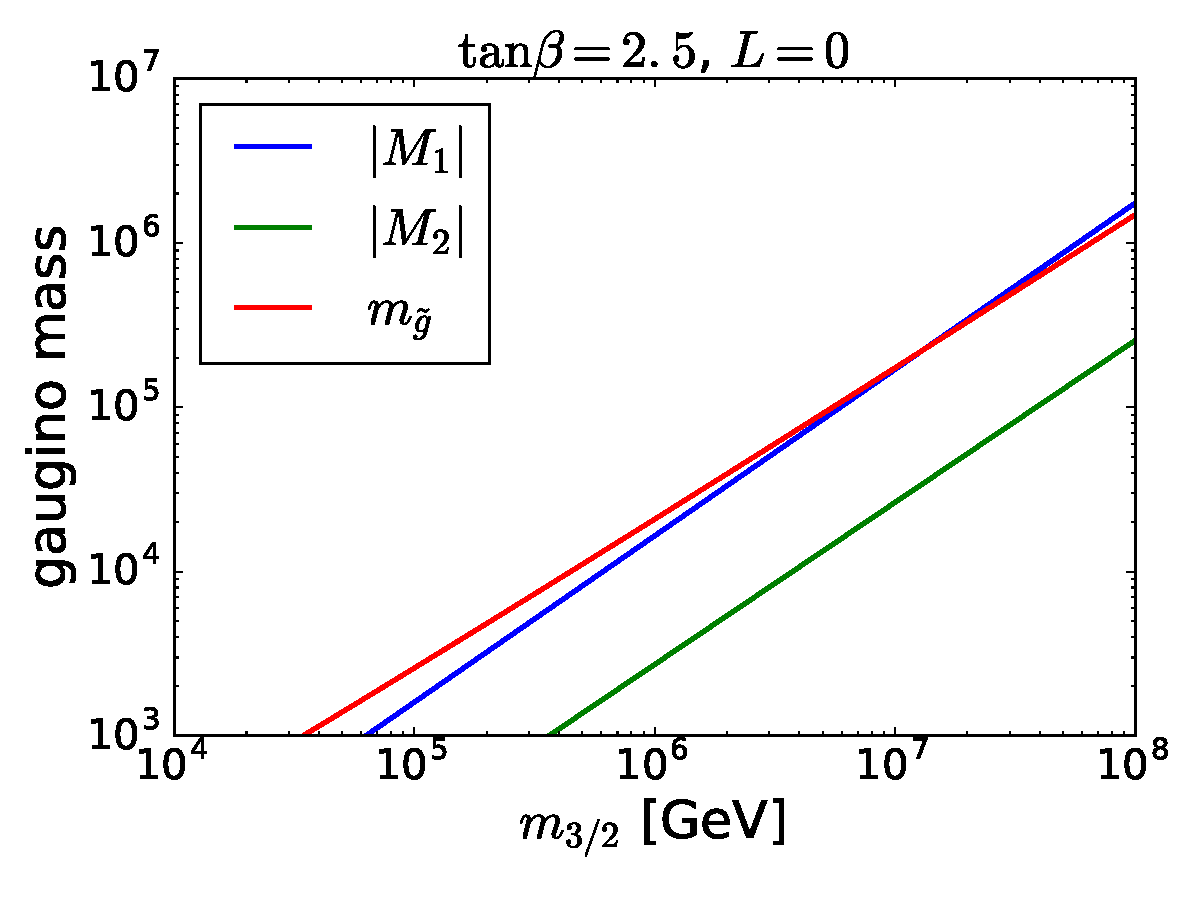
\includegraphics[width=0.48\hsize]{amsb_m32.pdf}
  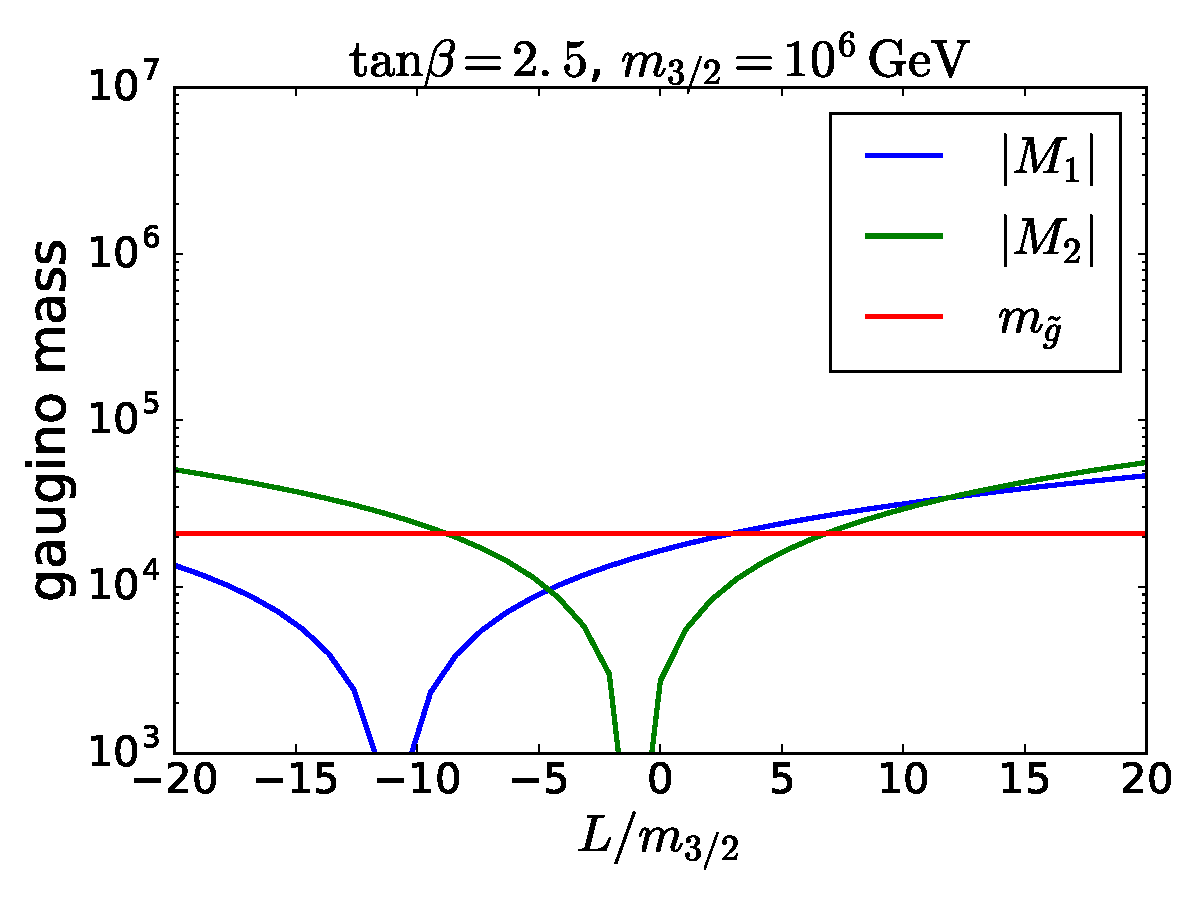
\includegraphics[width=0.48\hsize]{amsb_L.pdf}
  \caption{
    Gaugino masses as a function of $m_{3/2}$ with fixing $L = 0$ (left) and that of $L$ with fixing $m_{3/2} = 10^6\,\mathrm{GeV}$ (right).
    Blue, green, and red lines denote the masses of Bino, Wino, and gluino, respectively.
    $\tan\beta = 2.5$ is used in both figures.
  }
  \label{fig:amsb_spectrum}
\end{figure}

Below $M_S$, gaugino mass parameters further run towards the gaugino mass scale $M_{\tilde{G}}$, where the physical gaugino masses are determined.
Note that the bino and wino masses are roughly given by $|M_1 (M_{\tilde{G}})|$ and $M_2 (M_{\tilde{G}})$, while the gluino pole mass $m_{\tilde{g}}$ includes a sizable effect from the threshold correction as \cite{Giudice:2004tc}
\begin{align}
  m_{\tilde{g}} = |M_3 (M_{\tilde{G}})| \left[
  1 + \frac{g_3^2}{16\pi^2} \left( 12 + 9\ln \frac{M_{\tilde{G}}^2}{|M_3|^2} \right)
  \right].
\end{align}

In Fig.~\ref{fig:amsb_spectrum}, we show the dependence of gaugino masses on $m_{3/2}$ and $L$.
In the left panel, we take $\tan\beta = 2.5$ and $L=0$, and the $m_{3/2}$ dependence is shown.
Blue, green, and red lines denote the masses of Bino, Wino, and gluino, respectively.
We can see that, throughout the parameter region used here, Wino becomes the lighest gaugino, or the LSP that can be a dark matter candidate.
In this choice of parameters, $m_{3/2} = 10^6\,\mathrm{GeV}$ roughly corresponds to the observed value of the Higgs mass $m_h \sim 125\,\mathrm{GeV}$, which at the same time realizes the $\mathcal{O}(1)\,\mathrm{TeV}$ mass for Wino.
As we will see in Sec.~??, \rem{Caution!!} the Wino dark matter in this mass range is well-motivated since it gives us a collect relic abundance of the dark matter.

In the right panel of Fig.~\ref{fig:amsb_spectrum}, we also show the $L$ dependence of gaugino masses for $\tan\beta = 2.5$ and $m_{3/2} = 10^6\,\mathrm{GeV}$.
For simplicity, we neglect the relative phase of $m_{3/2}$ and $L$ and only consider the relative sign of them.
It can be seen that the hierarchy between gaugino masses is changed when a large value of $|L|$ is considered.
However, we can safely say that when the threshold correction is sufficiently small, $|L| \lsim \mathcal{O}(m_{3/2})$, Wino remains to be the LSP.
In addition, dependence of $m_h$ on $L$ is negligiblly small and $m_h$ changes only $\mathcal{O} (0.1)\,\mathrm{GeV}$ within the parameter choice of the right panel.


%%%%%%%%%%%%%%%%%%%%%%%%%%%%%%%%%%%%%%%%%%%%%%%%%%%%%%%%%%%%%%%%%%%%%%%%%%%%%%%
\subsection{Minimal dark matter model}
%%%%%%%%%%%%%%%%%%%%%%%%%%%%%%%%%%%%%%%%%%%%%%%%%%%%%%%%%%%%%%%%%%%%%%%%%%%%%%%

The minimal dark matter (MDM) \cite{Cirelli:2005uq, Cirelli:2007xd, Cirelli:2009uv} is another example model that contains a WIMP DM candidate.
This model attempts to explain the existence of the stable DM by extending the SM as simply as possible.
More specifically, we just assume the same gauge groups as the SM and add only one $SU(2)_L$ $n$-plet with/without $U(1)_Y$ hypercharge in the model.
The point is that, when $n$ is large, there are examples of multiplets that are sufficiently long-lived to be a DM candidate.

The stability can be understood through a simple group theoretical argument.
To write down the effective operator that describes the decay of the $n$-plet field, we have to make a $n$-plet representation out of several SM fields.
However, since the largest $SU(2)_L$ representation in the SM is doublet, we need at least $n-1$ SM fields in the operator.
The operator made out of this large number of fields should be suppressed by a power of the cutoff scale $\Lambda$, at least by $\Lambda^{4-n}$, and results in a small decay rate.

\rem{Possible choice of hypercharges}

% For some choice of charges and spin, such as the $n=5$ Majorana fermion without $U(1)_Y$ charge, even the existence of such operator is denied and the complete stability of the new particle is ensured.

\rem{About anomaly}


%%%%%%%%%%%%%%%%%%%%%%%%%%%%%%%%%%%%%%%%%%%%%%%%%%%%%%%%%%%%%%%%%%%%%%%%%%%%%%%
\subsection{Summary}
%%%%%%%%%%%%%%%%%%%%%%%%%%%%%%%%%%%%%%%%%%%%%%%%%%%%%%%%%%%%%%%%%%%%%%%%%%%%%%%

\begin{table}
  \centering
  \begin{tabular}{c|ccc|cc}
    & \multicolumn{3}{c|}{Quantum numbers} & \multicolumn{2}{c}{Masses}\\
    WIMP DM candidate & $SU(2)_L$ & $U(1)_Y$ & Spin & $m_\chi / \mathrm{TeV}$ &
    $\Delta m_\chi / \mathrm{MeV}$ \\
    \hline
    Higgsino & $2$ & $1/2$ & Dirac fermion & 1.1 & 341 \\
    Wino & $3$ & $0$ & Majorana fermion & 2.9 & 166 \\
    5-plet scalar & $5$ & $0$ & real scalar & 9.4 & 166 \\
    5-plet fermion & $5$ & $0$ & Majorana fermion & 10 & 166
  \end{tabular}
  \caption{
    Table of properties of WIMPs discussed in this thesis.
    In the ``Quantum numbers'' block, the $SU(2)_L$ and $U(1)_Y$ charges and spin nature are shown.
    In the ``Masses'' block, the proper mass of the thermally produced DM $m_\chi$ and mass difference between the neutral and charged components of the multiplet $\Delta m_\chi$ are shown.
    See Sec.~\ref{???} \rem{Caution!!} for the descriptions and implications of $m_\chi$ and Sec.~\ref{???} \rem{Caution!!} for those of $\Delta m_\chi$.
  }
  \label{tab:WIMP_property}
\end{table}

In Table~\ref{tab:WIMP_property}, we summarize the properties of WIMPs discussed in this thesis.
In the first block named ``Quantum numbers'', we show the $SU(2)_L$ electroweak charge, $U(1)_Y$ hypercharge, and spin nature.
In the second block named ``Masses'', two types of masses are shown.
$m_\chi$ is the required masses to explain the DM relic abundance without non-thermal production (see Sec.~?? \rem{Caution!!} for the detail).
$\Delta m_\chi$ is the mass difference between the electromagnetically neutral and charged components of the multiplet, as discussed in Sec.~?? \rem{Caution!!}.
Values of these masses are taken from \cite{Farina:2013mla, ArkaniHamed:2006mb, Hisano:2006nn,  Cirelli:2007xd, Moroi:2013sla, Beneke:2016ync}.


\bibliographystyle{elsarticle-num}
\bibliography{../phd}

\end{document}


\clearpage

% Erase biblio in input file before turning on
\documentclass[12pt,twoside,book]{article}
\usepackage{docmute}

\input{../settings}

\begin{document}

%%%%%%%%%%%%%%%%%%%%%%%%%%%%%%%%%%%%%%%%%%%%%%%%%%%%%%%%%%%%%%%%%%%%%%%%%%%%%%%
\section{WIMP as a dark matter}
\setcounter{equation}{0}
\label{sec:DM}
%%%%%%%%%%%%%%%%%%%%%%%%%%%%%%%%%%%%%%%%%%%%%%%%%%%%%%%%%%%%%%%%%%%%%%%%%%%%%%%

\vskip 0.1in

In this section, we review the properties of WIMPs as DM candidates.
It is revealed that, when we take a close look at the relic abundance of WIMP DM in Sec.~\ref{sec:relic}, a WIMP with the $\mathrm{TeV}$ scale mass is a good DM candidate, which is sometimes called \textit{WIMP miracle} and is a strong motivation to consider WIMPs.
In Sec.~\ref{sec:direct_detection} and Sec.~\ref{sec:indirect_detection}, we will consider two different ways to search for WIMP DM, called the direct and indirect detection.
Finally, Sec.~\ref{sec:summary_DM} is devoted to the summary and concluding remarks of this section.


%%%%%%%%%%%%%%%%%%%%%%%%%%%%%%%%%%%%%%%%%%%%%%%%%%%%%%%%%%%%%%%%%%%%%%%%%%%%%%%
\subsection{WIMP DM relic abundance}
\label{sec:relic}
%%%%%%%%%%%%%%%%%%%%%%%%%%%%%%%%%%%%%%%%%%%%%%%%%%%%%%%%%%%%%%%%%%%%%%%%%%%%%%%

One of the most important evidence of the beyond SM phenomena is the existence of DM \cite{Zwicky:1933}.
DM is an unknown object that occupies a large fraction of the total energy of our universe but has not yet been directly observed because of its weak interaction with the SM particles.\footnote{
  At worst DM interacts with the SM particles through gravity, which is considerably weaker than all the other known interactions.
}
In spite of its invisibility, the existence of DM is confirmed by several astrophysical observations such as the mass measurement using the gravitational lensing effect caused by galaxies and clusters \cite{Zwicky:1937, Trimble:1987ee}, the flatness of galactic rotation curves beyond the optical radius \cite{1939LicOB..19...41B, Begeman:1991iy}, the measurement of the power spectrum of the cosmic microwave background (CMB), and so on.
In particular, the observation of CMB allows us the precise determination of various cosmological parameters \cite{Jungman:1995av, Jungman:1995bz} including the normalized density of the non-relativistic matter $\Omega_m$ and that of baryon $\Omega_b$, which is currently determined as \cite{Aghanim:2018eyx}
\begin{align}
  \Omega_m h^2 &= 0.1430 \pm 0.0011,\\
  \Omega_b h^2 &= 0.02237 \pm 0.00015,
\end{align}
where $h \sim 0.7$ is the Hubble constant in units of $100\, \mathrm{km}\, \mathrm{s}^{-1}\, \mathrm{Mpc}^{-1}$.
The difference between $\Omega_m h^2$ and $\Omega_b h^2$ implies the existence of DM and its abundance $\Omega_\chi h^2 \simeq 0.12$.

In cosmology, DM production mechanisms that explain the DM abundance are divided into two large categories: thermal and non-thermal production.
The former assumes the equilibrium between the DM and the SM thermal bath in the early universe.
As the universe expands, the interaction rate that maintains the thermal equilibrium becomes smaller and the DM decouples from the thermal bath at some time, which is the so-called \textit{freezeout}.
As we will see below, the resulting abundance of the DM in this scenario is mainly controlled by the thermal averaged annihilation cross section $\Braket{\sigma v}$.
On the other hand, non-thermal production assumes the DM production by some processes irrespective of the thermal bath such as the decay of a heavy particle.
From now on, we mainly focus on the case without the non-thermal production, which still gives some relic abundance for WIMPs that have an interaction with the SM thermal bath through the electroweak interaction.

We assume the stable DM particle $\chi$ with mass $m_\chi$ that pair annihilates into SM particles with some cross section $\sigma$.
When DM is in thermal equilibrium with the thermal bath of temperature $T$, DM velocity obeys the corresponding Boltzmann distribution.
Let $v$ be the relative velocity of annihilating DM particles and $\Braket{\sigma v}$ be the thermal average of the product of $\sigma$ and $v$.
By using this quantity, we can write down the Boltzmann equation for the DM number density $n_\chi$ in a simplified approximation as
\begin{align}
  \frac{d (n_\chi a^3)}{d t} =
  - a^3 \Braket{\sigma v} (n_\chi^2 - n_{\mathrm{eq}}^2),\label{eq_boltzmann}
\end{align}
where $t$ and $a$ are the time coordinate and the scale factor, respectively, of the Friedmann Robertson Walker metric
\begin{align}
  d s^2 = - d t^2 + a(t)^2 d \bm{x}^2,
\end{align}
while $n_{\mathrm{eq}}$ denotes the number density of DM in equilibrium.
When DMs are non-relativistic, its temperature dependence is given by $n_{\mathrm{eq}} \propto T^{3/2} \exp \left( -m_\chi / T \right)$.
The first term of the right-handed side of Eq.~\eqref{eq_boltzmann} represents the annihilation rate of DM pairs that should be proportional to $n_\chi^2$, while the second term describes the DM creation through the inverse process.
As desired, the comoving number density does not change in time if $n_\chi = n_{\mathrm{eq}}$.
Recalling the total entropy conservation in a comoving volume $s a^3 = (\mathrm{const})$, it turns out to be convenient to define the ratio $Y \equiv n_\chi / s$.
In fact, this modification cancels the effect of the expansion of the universe $da / dt > 0$ from Eq.~\eqref{eq_boltzmann}, leading to a simpler equation
\begin{align}
  \frac{d Y}{d t} =
  -s \Braket{\sigma v} (Y^2 - Y_{\mathrm{eq}}^2),\label{eq_boltzmann_Yt}
\end{align}
with $Y_{\mathrm{eq}} \equiv n_{\mathrm{eq}} / s$.

Here, we assume that the freezeout occurs when the relativistic radiation dominates the total energy of the universe, which will be verified to be correct later.
In this case, we can derive $a \propto T^{-1}$ from the entropy conservation with $s \propto T^3$.
For the numerical calculation, we define a dimensionless parameter $x \equiv m_\chi / T$.
Then Eq.~\eqref{eq_boltzmann_Yt} can be rewritten as
\begin{align}
  \frac{x}{Y_{\mathrm{eq}}} \frac{d Y}{d x} =
  -\frac{\Gamma}{H} \left( \frac{Y^2}{Y_{\mathrm{eq}}^2} - 1 \right),\label{eq_boltzmann_Yx}
\end{align}
where $\Gamma$ denotes the DM interaction rate defined as
\begin{align}
  \Gamma &\equiv n_{\mathrm{eq}} \Braket{\sigma v}.\label{eq_lambda}
\end{align}

\begin{figure}[t]
  \centering
  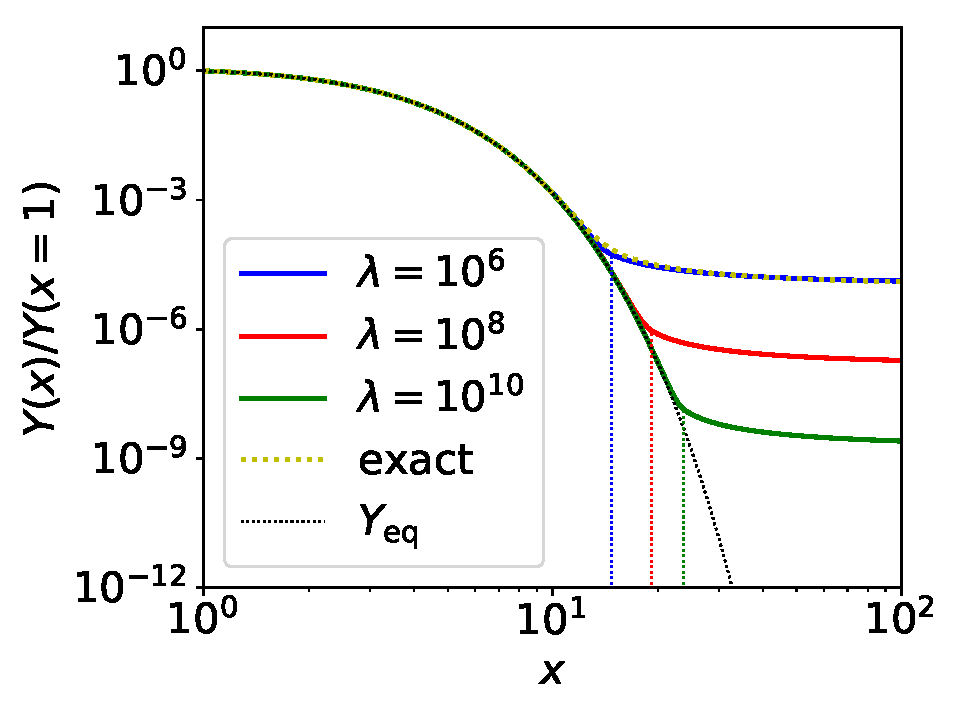
\includegraphics[width=0.5\hsize]{DMrelic.pdf}
  \caption{
    Plot of $Y(x) / Y(x=1)$ with $Y(x)$ being a solution of the evolution equation Eq.~\eqref{eq_boltzmann_Yx}.
    The yellow dotted line is a solution for $\lambda \equiv \left. \Gamma / H \right|_{x=1} = 10^6$, while the black dotted line shows $Y_{\mathrm{eq}} (x) / Y_{\mathrm{eq}} (x=1)$.
    The solid lines are the approximation to the solutions described in the text.
    The blue, red, and green colors correspond to $\lambda = 10^6$, $10^8$, and $10^{10}$, respectively.
    The vertical dotted lines denote the freezeout temperature $x_f$.
  }
  \label{fig_DM_relic}
\end{figure}

Finally, it is known that $\Braket{\sigma v}$ can be expanded as~\cite{Gondolo:1990dk}
\begin{align}
  \Braket{\sigma v} = \Braket{\sigma v}_s +
  \Braket{\sigma v}_p x^{-1} + \cdots,
\end{align}
corresponding to the $s$-wave, $p$-wave, and so on, contributions to the cross section.
When $x \gg 1$, which is the same as the non-relativistic limit, the term with the highest power of $x$ dominates the cross section.  When the $x^{-p}$ term dominates ($p \geq 0$), the temperature dependence of the interaction rate is $\Gamma \propto x^{-3/2-p} e^{-x}$, while the Hubble parameter only reduces as $H \propto \rho^{1/2} \propto x^{-2}$.
As a result, at some point $\Gamma$ becomes smaller than $H$ and $Y$ freezes out as Eq.~\eqref{eq_boltzmann_Yx} indicates.
Hereafter, we focus on the case of the $s$-wave domination with $\Braket{\sigma v}_s \neq 0$ for simplicity.
In Fig.~\ref{fig_DM_relic}, we show the solution of Eq.~\eqref{eq_boltzmann_Yx} for $\lambda \equiv \left. \Gamma / H \right|_{x=1} = 10^6$ by the yellow dotted line.
In the calculation, we use the boundary condition $Y(x=1) = Y_{\mathrm{eq}} (x=1)$ and plot the normalized value $Y(x) / Y(x=1)$.  We also plot the function $Y_{\mathrm{eq}} (x) / Y_{\mathrm{eq}} (x=1)$ by the black dotted line.

Unfortunately, it is computationally hard to solve Eq.~\eqref{eq_boltzmann_Yx} for larger values of $\lambda$ because of the almost complete cancellation between two terms of the right-handed side for small $x\sim \mathcal{O}(1)$ and its amplification caused by large $\lambda$.
We adopt instead to use an approximation that is the same as the one adopted in the public code \texttt{MicrOMEGAs}~\cite{Belanger:2001fz, Belanger:2018mqt}.
For the small $x$ region, the temperature is still high enough to maintain the equilibrium $Y \simeq Y_{\mathrm{eq}}$, which means that $d \Delta Y / d x \ll d Y_{\mathrm{eq}} / d x$ with $\Delta Y \equiv Y - Y_{\mathrm{eq}}$.
From this approximation, we obtain a formula
\begin{align}
  \Delta Y \simeq -\frac{x}{2 \lambda} \frac{d Y_{\mathrm{eq}}}{d x}.\label{eq_relic_app_1}
\end{align}
Then we define the time $x_f$, or equivalently the freezeout temperature $T_f$, when the approximation becomes invalid through the equation\footnote{
  One can easily check that the final relic abundance is not sensitive to the choice of the numerical coefficient $2.5$ in Eq.~\eqref{eq:freezeout_temperature}.
}
\begin{align}
  \Delta Y (x_f) = 2.5 Y_{\mathrm{eq}} (x_f).
  \label{eq:freezeout_temperature}
\end{align}
After the freezeout $x > x_f$, the annihilation of the DM pairs rapidly slows down and the DM abundance far exceeds its equilibrium value: $Y \gg Y_{\mathrm{eq}}$.
Then we can neglect the second term of the right-handed side of Eq.~\eqref{eq_boltzmann_Yx} and obtain the analytical solution
\begin{align}
  Y(x) \simeq - \frac{x}{c_1 x + \lambda / Y_{\mathrm{eq}} (x=1)},\label{eq_relic_app_2}
\end{align}
where $c_1$ is an integration constant.
In Fig.~\ref{fig_DM_relic}, we show results obtained with these two approximations Eqs.~\eqref{eq_relic_app_1} and \eqref{eq_relic_app_2} for $\lambda = 10^6$ (blue), $10^8$ (red), and $10^{10}$ (green).
In particular, the blue and the yellow lines almost completely overlap with each other, which proves the validity of the approximations.
The vertical dotted lines in the figure show the freezeout temperature.
It can be seen from the figure that $x = x_f$ does correspond to the time when $Y$ starts to deviate from $Y_{\mathrm{eq}}$.
Note also that as $\lambda \propto \Braket{\sigma v}$ becomes larger, the freezeout time becomes later and the resulting relic abundance becomes smaller.
It is known that for typical WIMPs with $m_\chi \sim \mathcal{O}(1)\mathrm{TeV}$, $\lambda \sim 10^8$ and thus $T_f \simeq m_\chi / 20$ from the figure.
Then, the freezeout temperature is much larger than the temperature at the radiation-matter equality, and we can confirm that the assumption of the radiation dominated universe at the time of the freezeout is correct.

When the DM properties (\textit{i.e.}, the mass $m_\chi$ and the annihilation cross section $\Braket{\sigma v}$ for a given temperature $T$) are given, corresponding relic abundance can be calculated using above procedure.
In particular, $m_\chi$ determines the normalization of the figure, namely $Y_{\mathrm{eq}} (x=1) = Y_{\mathrm{eq}} (T=m_\chi)$, and $\Braket{\sigma v}$ determines the freezeout temperature through the combination of Eq.~\eqref{eq_lambda}.
Assuming the absence of a non-thermal production, there should be a unique choice of $m_\chi$ corresponding to some $\Braket{\sigma v}$ to explain the current relic abundance of the DM.
From the numerical calculation, we obtain an order estimation formula
\begin{align}
  \Omega_\chi h^2 \sim \frac{3 \times 10^{-27}\,\mathrm{cm^3}/\mathrm{s}}
  {\Braket{\sigma v}_0} \sim
  0.1 \left( \frac{0.01}{\alpha} \right)^2
  \left( \frac{m_\chi}{300\,\mathrm{GeV}} \right)^2,\label{eq_relic_abundance}
\end{align}
where the rough estimation $\Braket{\sigma v} \sim \alpha^2/m_\chi^2$ is used in the last equation with $\alpha$ being the fine structure constant for the DM-SM coupling.
What is fascinating in Eq.~\eqref{eq_relic_abundance} is that a particle can be DM if it has a mass comparable to the electroweak scale and coupling constant comparable to the electroweak coupling constant.
This is the so-called \textit{WIMP miracle}, which supports the hypothesis of the WIMP as a candidate of the DM.
Such $\mathrm{TeV}$-scale WIMPs are theoretically well-motivated in connection with problems of the SM such as the naturalness problem as reviewed in Sec.~\ref{sec:model}.
Also, phenomenologically such $\mathrm{TeV}$-scale WIMPs are of great interest, since they can be detected using several different methods as will be described in this thesis.

In Table \ref{tab:WIMP_property}, we summarize the value of $m_\chi$ for each WIMP model that predicts the correct relic abundance $\Omega_\chi h^2 \sim 0.12$.
As described above, $\mathrm{TeV}$ scale masses are suitable for all WIMP DMs and the required mass becomes larger when we consider a larger $SU(2)_L$ $n$-plet because of the larger annihilation cross section.
However, note that the precise estimation of the relic abundance solely using the last term of Eq.~\eqref{eq_relic_abundance} is not possible, because of the so-called Sommerfeld enhancement effect \cite{Hisano:2004ds,Hisano:2006nn} that may significantly modify the annihilation cross section.
We will review this effect in more detail in Sec.~\ref{sec:indirect_detection} in relation to the indirect detection experiments.
Note also that $m_\chi$ in the table is only an upper bound on the WIMP DM mass because the existence of non-thermal production processes may allow lighter WIMPs to explain the whole relic abundance of DM in the current universe.


%%%%%%%%%%%%%%%%%%%%%%%%%%%%%%%%%%%%%%%%%%%%%%%%%%%%%%%%%%%%%%%%%%%%%%%%%%%%%%%
\subsection{WIMP DM search : direct detection}
\label{sec:direct_detection}
%%%%%%%%%%%%%%%%%%%%%%%%%%%%%%%%%%%%%%%%%%%%%%%%%%%%%%%%%%%%%%%%%%%%%%%%%%%%%%%

There are many experiments aimed at the direct detection of the DM\footnote
{
  For a recent review of the direct detection experiments, see for example \cite{Undagoitia:2015gya}.
}
proposed in \cite{Goodman:1984dc}.
Here, we assume some interaction between the DM and SM particles and look for the recoil of a target SM particle due to the collision with the DM in the laboratory.
In the case of WIMPs of our concern, any particle with non-zero electroweak charges can be a target particle, which interacts with WIMPs through the $t$-channel electroweak gauge boson exchange.
In the traditional setup such as the XENON1T experiment \cite{Aprile:2012zx}, a nucleus (of xenon in XENON1T) and an electron are the frequently used target particles.
From now on, we focus on the nucleus target since, as we will see later, it gives much better sensitivity than the electron target for DMs with a mass of $\mathcal{O} (\mathrm{TeV})$.
In this case, there are several ways to read out the information of the nuclear recoil depending on the deposited energy, such as the use of heat (or photons), an excitation of the nucleus associated with the emission of scintillation light, and the ionization of the atom.
Among them, the XENON1T experiment uses the scintillation light and the ionization.

To evaluate the event rate for this kind of experiment, it is important to know the DM energy density $\rho_0$ and velocity distribution around us.
For this purpose, we model the DM profile in our galaxy using the so-called standard halo model (SHM) and adjust the parameters to the observations.
In the SHM, we assume the DM velocity distribution in the galactic rest frame
\begin{align}
  f(\bm{v}) = \frac{1}{\sqrt{2\pi \sigma}} \exp \left[ -\frac{\bm{v}^2}{2 \sigma^2} \right],
\end{align}
with $\sigma \equiv \sqrt{3/2} v_c$, where $v_c$ denotes the local circular speed of DMs around the Galactic Center.
From the combination of different analyses, we obtain the values $\rho_0 = 0.3\,\mathrm{GeV / cm^3}$ and $v_c = 220\,\mathrm{km/s}$ \cite{Kerr:1986hz,Green:2011bv}.
Also, the DM velocity within the halo cannot be arbitrarily large, since such energetic DM will not be gravitationally bound and will escape from our galaxy.
Correspondingly, we often introduce a cutoff velocity $v_{\mathrm{esc}} = 544\,\mathrm{km / s}$ \cite{Smith:2006ym} and simply assume $f(\bm{v}) = 0$ for $|\bm{v}| > v_{\mathrm{esc}}$.

Using the distribution defined above, the differential event rate per unit recoil energy $E$ per unit material mass is given by \cite{Lewin:1995rx}
\begin{align}
  \frac{d R}{d E} (E,t) = \frac{\rho_0}{m_\chi m_T} \int d^3 v\, v f(\bm{v}, t)
  \frac{d \sigma}{d E} (E, v),
  \label{eq:rate}
\end{align}
where $m_T$ is the mass of the target nucleus, while $d\sigma / dE$ is the differential cross section of the DM-nucleus scattering.
The DM velocity distribution $f(\bm{v}, t)$ is now time-dependent since it represents the distribution observed at the laboratory, which is affected by the motion of the Earth around the Sun and that of the Sun around the Galactic Center.
Thus, $f(\bm{v}, t)$ is derived by performing the Galilean transformation to $f(\bm{v})$ according to the time-dependent velocity of the Earth against the galactic rest frame.
This time-dependence gives the signal a characteristic daily and yearly modulation, which helps us to distinguish it from the background events.
Also, the Galilean transformation makes $f(\bm{v}, t)$ highly anisotropic since the velocity of the Earth is comparable to $v_c$.
Thus, if it is possible to use the directional information, it also helps us to reduce the background.

The differential cross section $d\sigma / dE$, which summarizes the particle physics part of the calculation, is divided into two parts: the spin-independent (SI) part and the spin-dependent (SD) part.
Denoting the SI and SD scattering cross sections for zero momentum transfer as $\sigma_0^{\mathrm{SI}}$ and $\sigma_0^{\mathrm{SD}}$, respectively, we obtain
\begin{align}
  \frac{d\sigma}{d E} (E, v) = \frac{m_T}{2 \mu_T^2 v^2}
  \left( \sigma_0^{\mathrm{SI}} F_{\mathrm{SI}}^2 (E)
  + \sigma_0^{\mathrm{SD}} F_{\mathrm{SD}}^2 (E) \right),
\end{align}
with $\mu_T$ being the reduced mass of the WIMP-nucleus system.
The form factors $F_{\mathrm{SI}}$ and $F_{\mathrm{SD}}$ summarize the nuclear physics part of the matrix element, both of which have properties $F(0)=1$ and $dF / dE < 0$ for large $E$.
Among SI and SD contributions, the SI part is of great interest thanks to the possible coherent enhancement of the cross section.
When the de Broglie wavelength corresponding to the momentum transfer $q$ is longer than the size of the nucleus (corresponding to $q \lesssim 200\,\mathrm{MeV}$ for the xenon), not the individual neutrons and protons but the whole nucleus contribute to the cross section.\footnote{
  When the DM is lighter and the de Broglie wavelength is even longer, the collective excitation modes of nuclei or electrons such as the phonon becomes important (see for example \cite{Knapen:2017xzo}).
  This corresponds to $q \lesssim \mathcal{O}(1)\,\mathrm{keV}$ or $m_\chi \lesssim \mathcal{O}(1)\,\mathrm{MeV}$ and thus we neglect this possibility here.
}
This results in the coherent contribution from all nucleons for the SI case, while only the unpaired nucleons contribute to the cross section for the SD case.
In fact, for the WIMP DM, the SI cross section $\sigma_0^{\mathrm{SI}}$ is enhanced thanks to the coherence by a large factor $A$ that is the mass number of the target nucleus ($A \simeq 130$ for the xenon) as
\begin{align}
  \sigma_0^{\mathrm{SI}} = A^2 \sigma_p^{\mathrm{SI}} \frac{\mu_T^2}{\mu_p^2}
\end{align}
where $\sigma_p^{\mathrm{SI}}$ is the SI scattering cross section for a DM and a single nucleon and $\mu_p$ is the reduced mass of the WIMP-nucleon system.
The above expression dominates over the SD cross contribution for the WIMP DM for most cases.

\begin{figure}[t]
  \centering
  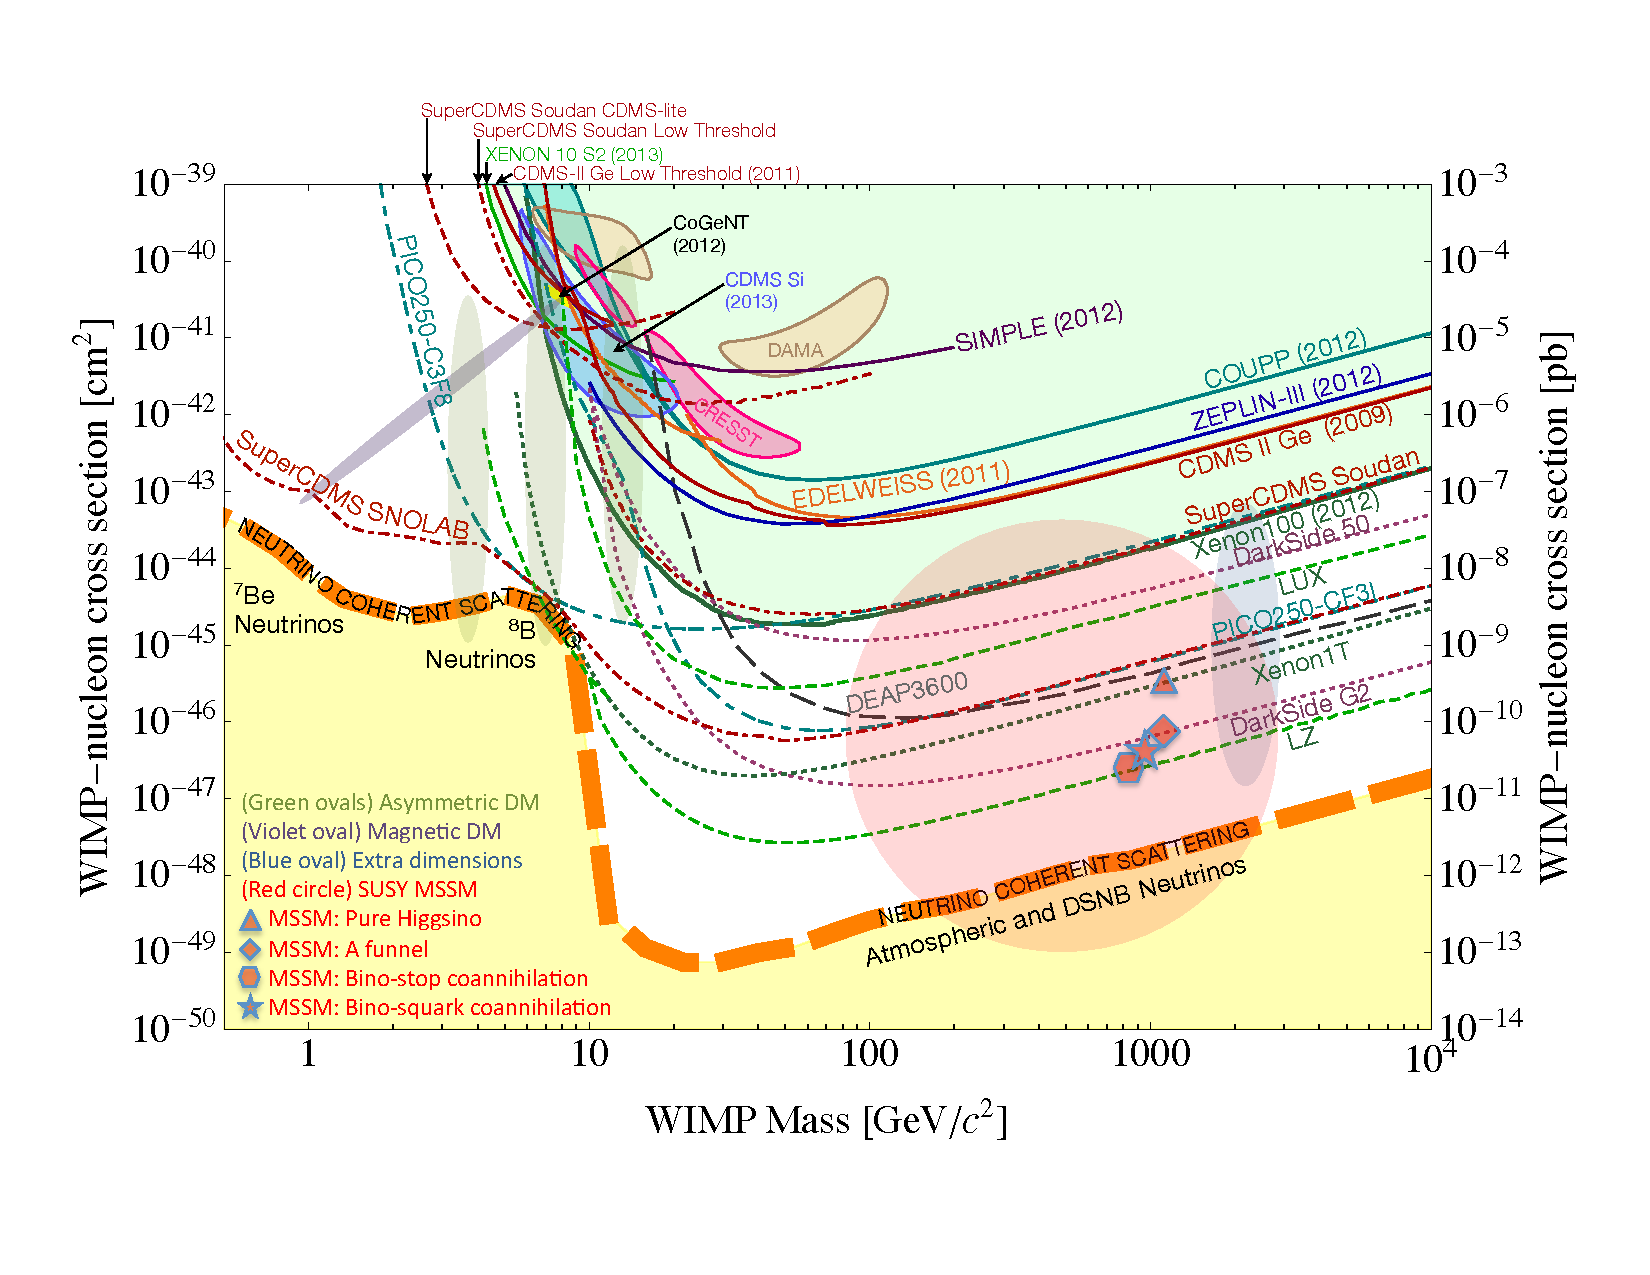
\includegraphics[width=0.8\hsize]{SNOWMASS_LimitPlot_SI_v3.pdf}
  \caption{
    Current constraints and prospects on the DM SI cross section taken from \cite{Cushman:2013zza}.
    The $y$-axis corresponds to $\sigma_p^{\mathrm{SI}}$ in our notation.
  }
  \label{fig:XENON1T}
\end{figure}

In Fig.~\ref{fig:XENON1T}, we show the current constraints and prospects on the DM SI scattering cross section $\sigma_p^{\mathrm{SI}}$ as a function of its mass.
See \cite{Cushman:2013zza} and references therein for the details of each experiment.
In the figure, the parameter region above each line is excluded and the orange dashed line represents the cross section of the background events sourced by neutrinos \cite{Billard:2013qya}.
This background often called as the neutrino floor, which is mainly determined by the solar neutrino for the region $m_\chi \lesssim 10\,\mathrm{GeV}$ and by the atmospheric and supernova neutrinos for $m_\chi \gtrsim 10\,\mathrm{GeV}$, roughly represents the maximum possible sensitivity of the direct detection method.\footnote{
  It may be possible, in particular for the solar neutrino background, to significantly reduce the number of background events and go beyond the neutrino floor by using the directional information of the signals.
}
Currently, the XENON1T collaboration~\cite{Aprile:2018dbl} provides the most stringent constraint in the (sub-)$\text{TeV}$ region of our interest.
Prospects of future planned experiments called DarkSide G2 \cite{Aalseth:2015mba} and LZ \cite{Mount:2017qzi} are also shown in the figure.

The qualitative description of the form of the sensitivity curves in Fig.~\ref{fig:XENON1T} can be given using the above discussion.
The sensitivity for a very light WIMP is weak because of the finite threshold $E_{\mathrm{thr}}$ of the recoil energy required for the detection of the signal.
The threshold effect can be taken into account by choosing the lower boundary of the $\bm{v}$-integral in Eq.~\eqref{eq:rate} to be $v_{\mathrm{min}}$ defined as
\begin{align}
  v_{\mathrm{min}} = \sqrt{\frac{m_T E_{\mathrm{thr}}}{2 \mu_T^2}}.
\end{align}
Since $v_{\mathrm{min}} \propto m_\chi^{-1}$ for $m_\chi \ll m_T$, the event rate rapidly becomes smaller for smaller $m_\chi$.
On the other hand, heavier WIMP DMs have less number density with the energy density $\rho_0$ fixed.
Because of this, the sensitivity for a heavy WIMP becomes moderately worse when $m_\chi$ increases.
These two behaviors determine the best suitable $m_\chi$ for each choice of $m_T$ and $E_{\mathrm{thr}}$, which is the reason why the xenon nucleus target is more suitable for the $\mathrm{TeV}$-scale WIMP search than the electron target.
The latter choice is suitable when we search for lighter DMs.

Although no signal of DM is observed yet, this null result is still consistent with WIMP models of our concern.
For example, the Wino DM scatters with a nucleon through the t-channel exchange of a higgs boson or two $W$ gauge bosons at the one-loop order or higher.
The calculation of the scattering cross section up to the next-to-leading order in $\alpha_s$ reveals that it almost mass-independently takes a small value of $\sigma_p^{\mathrm{SI}} \simeq 2.3 \times 10^{-47}\,\mathrm{cm}^2$~\cite{Hisano:2015rsa}, which is below the current constraint but is a region of future interest.
As for the MDM, the $5$-plet fermion is analyzed in \cite{Hisano:2011cs} and the scattering cross section $\sigma_p^{\mathrm{SI}} \simeq 10^{-46}\,\mathrm{cm}^2$ is obtained.
However, the mass requirement $m_\chi \sim 10\,\mathrm{TeV}$ (see Table~\ref{tab:WIMP_property}) makes the detection difficult and the sensitivity will not cover the whole region of the viable parameter space.
In general, a pure $SU(2)_L$ multiplet with non-zero hypercharge has a large contribution to $\sigma_p^{\mathrm{SI}}$ from the tree-level exchange of $Z$ boson \cite{Farina:2013mla}.
Thus, for such a particle to be a viable DM candidate, we should modify the model to forbid the tree-level scattering.
Related to this point, the Higgsino-like DM is a kind of a mixed multiplet that can avoid the tree-level scattering via $Z$ boson.
As is discussed in Sec.~\ref{sec:mass_splitting}, the mixing between Higgsino and gauginos splits the masses of two neutral components of the Higgsino-like state, making them two Majorana fermions.
If the size of the mass splitting is larger than the typical kinetic energy of the Higgsino-like DM, the scattering with t-channel $Z$ boson exchange is suppressed and the loop-suppressed scattering cross section for the direct detection dominates.
This argument sets an upper bound on the lighter electroweak gaugino mass $M_i$ ($i=1,2$) as $\Braket{\mu v^2} \lesssim M_Z^2 / M_i$.
By substituting $\mu = 1\,\mathrm{TeV}$ and $v \sim 10^{-3}$, we obtain $M_i \lesssim 10^7\,\mathrm{GeV}$ from the direct detection constraint.
Under this constraint, the phenomenology of the Higgsino-like state is still highly model-dependent since the size of the mixing significantly modifies the scattering cross section.
According to \cite{Hisano:2012wm, Roszkowski:2014wqa}, the almost pure Higgsino has $\sigma_p^{\mathrm{SI}}$ below the neutrino floor, while some of the parameter space with a sizable mixing has much larger $\sigma_p^{\mathrm{SI}}$ that is already excluded.
Thus, we conclude that the almost pure Higgsino is difficult to search for using this method.


%%%%%%%%%%%%%%%%%%%%%%%%%%%%%%%%%%%%%%%%%%%%%%%%%%%%%%%%%%%%%%%%%%%%%%%%%%%%%%%
\subsection{WIMP DM search : indirect detection}
\label{sec:indirect_detection}
%%%%%%%%%%%%%%%%%%%%%%%%%%%%%%%%%%%%%%%%%%%%%%%%%%%%%%%%%%%%%%%%%%%%%%%%%%%%%%%

The indirect detection of DM\footnote{
  For a recent review of the indirect detection experiments, see for example \cite{Gaskins:2016cha}.
}
uses the DM annihilation process into SM particles to detect the DM signal.
When DM is composed of WIMPs, their annihilation can be again explained by the electroweak interaction.
Since DMs are non-relativistic in the current universe, the $s$-wave contribution to the annihilation cross section, if exists, dominates over others, which results in the dominant annihilation process coming from the $t$- and $u$-channel exchange of a virtual WIMP.
Then, some of the final state particles may propagate to the earth and be observed by telescopes in the form of gamma-rays, neutrinos, cosmic rays, and so on.

The DM annihilation rate at some point $\bm{x}$ of the universe has a quadratic dependence on the local DM energy density $\rho_\chi (\bm{x})$.\footnote{
  More precisely, the annihilation rate has a quadratic dependence on the DM number density $n_\chi (\bm{x})$.
  This means that, for some fixed value of $\rho_\chi (\bm{x})$, the lighter DM has more chance to annihilate since $n_\chi = \rho_\chi / m_\chi$.
}
In our case, we focus on the photons produced at the WIMP annihilation, and the main targets of indirect detection experiments are the center of galaxies or galaxy clusters, where abundant DM is expected to be accumulated thanks to the strong gravitational potential.
The DM energy density distribution around each galaxy (cluster) can be determined by the observation of the rotation curve of luminous objects.
One of the model functions introduced to fit such observations is the so-called the Navarro-Frenk-White (NFW) profile \cite{Navarro:1995iw, Navarro:1996gj} of the DM density distribution,
\begin{align}
  \rho_{\mathrm{NFW}} (r) = \frac{\rho_s}
  { \left( \frac{r}{r_s} \right) \left[ 1 + \left( \frac{r}{r_s} \right) \right]^2},
\end{align}
where $r$ is the distance from the center of the galaxy of our concern.
Free parameters $\rho_s$ and $r_s$ should be chosen to fit the data for each galaxy, which gives for our galaxy $\rho_s \sim 1\times 10^7 M_\odot\, \mathrm{kpc}^{-3}$ and $r_s \sim 20\,\mathrm{kpc}$ \cite{Fornasa:2013iaa} with $M_\odot$ being the solar mass.

\begin{figure}
  \centering
  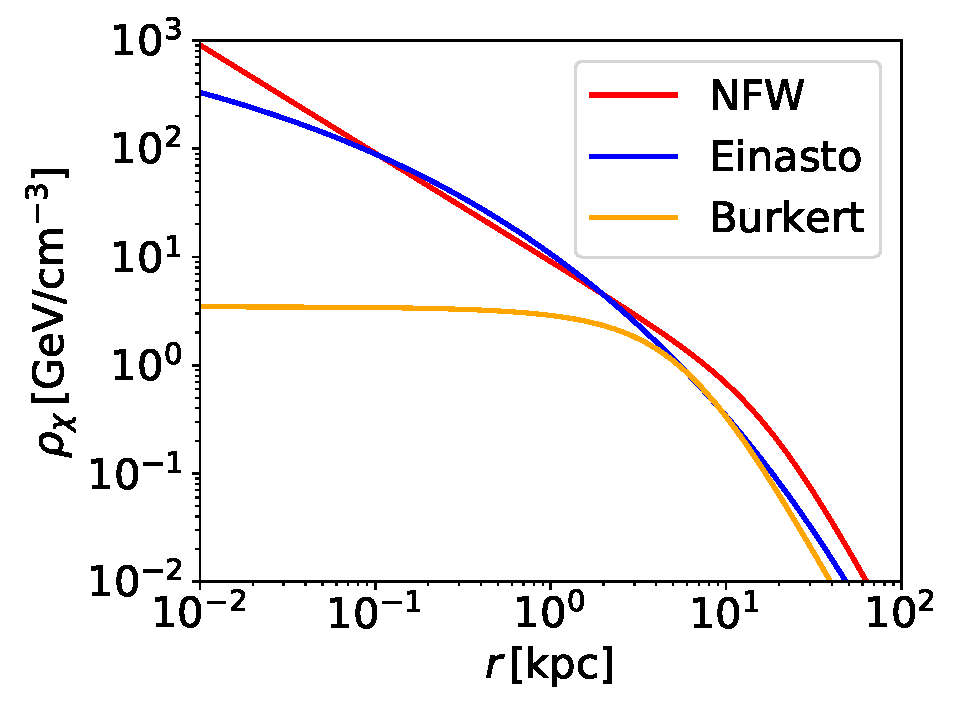
\includegraphics[width=0.5\hsize]{profile.pdf}
  \caption{
    Dark matter energy density $\rho_\chi$ within our galaxy as a function of the distance from the galactic center $r$.
  }
  \label{fig:profile}
\end{figure}

The inner slope of the NFW profile follows $\rho_{\mathrm{NFW}} \propto r^{-1}$.
On the other hand, many observations of the rotation curve and models of dwarf galaxies suggest the scaling behavior $\rho \propto r^0$, which is the so-called core-cusp problem (see \cite{Genina_2017} and references therein).
To take account of this behavior, other profiles are also widely used: the Einasto profile \cite{1965TrAlm...5...87E, Graham:2005xx}
\begin{align}
  \rho_{\mathrm{Einasto}} (r) = \rho_s \exp \left[
  -\frac{2}{\alpha} \left\{ \left( \frac{r}{r_s} \right)^\alpha - 1 \right\} \right],
\end{align}
with $\rho_s \sim 5 \times 10^6 M_\odot\, \mathrm{kpc}^{-3}$, $\alpha \sim 0.2$, and $r_s \sim 10\,\mathrm{kpc}$ for our galaxy, and the Burkert profile \cite{Burkert:1995yz}
\begin{align}
  \rho_{\mathrm{Burkert}} (r) = \frac{\rho_s}
  {\left( 1 + \frac{r}{r_s} \right) \left( 1 + \frac{r^2}{r_s^2} \right)},
\end{align}
with $\rho_s \sim 9 \times 10^7 M_\odot\, \mathrm{kpc}^{-3}$ and $r_s \sim 6\, \mathrm{kpc}$ for our galaxy.
In Fig.~\ref{fig:profile}, we show the DM energy density distribution in our galaxy.\footnote{
  In principle, all the profiles should reconstruct the DM density at the Sun $\rho (r \sim 8\, \mathrm{kpc}) \sim 0.3\, \mathrm{GeV} / \mathrm{cm}^3$, which is apparently not the case.
  This deviation can be explained by the effect of the fitting error, which results in an order of magnitude uncertainty in $\rho_\chi$ at the $68\,\%$ level.
}
As for the choice of parameters, we use the mean values of fits of several observations listed in \cite{Fornasa:2013iaa}.
We can see the difference in shapes among three profiles at the small $r$ region.

Next we derive the formula to estimate the event rate of the indirect detection experiments.
The event rate at the laboratory can be divided into the particle physics part and the astrophysical part, the second of which, referred to as the $J$-factor, is related to the DM density distribution.
The $J$-factor for the DM annihilation for a sky patch with solid angle $\Delta\Omega$ around a sky direction $\hat{\bm{n}}$ is given by
\begin{align}
  J(\hat{\bm{n}}, \Delta\Omega) = \int_{\Omega \sim \hat{\bm{n}}} d\Omega
  \int_{\mathrm{LOS}} \rho_\chi^2 (\Omega, \ell) d\ell,
  \label{eq:J-factor}
\end{align}
where $\ell$ is a distance along the line-of-sight (LOS) defined by the direction $\Omega$.
The first integration performed over a region $\Delta\Omega$ around the direction $\hat{\bm{n}}$, while the second one sums up all the contributions from DMs on the LOS.
Using this, the flux $\Phi_x(E, \hat{\bm{n}}, \Delta\Omega)$ of a SM particle $x$ with energy $E$ at the sky patch is expressed as\footnote{
  We identify the DM particle and anti-particle in the calculation of Eq.~\eqref{eq:flux}.
  If this is not the case, the right-handed side should be multiplied by an extra factor of $1/2$.
}
\begin{align}
  \Phi_x (E, \hat{\bm{n}}, \Delta\Omega) = \frac{\Braket{\sigma v}}{8\pi m_\chi^2}
  \frac{d N_x}{d E} J(\hat{\bm{n}}, \Delta\Omega),
  \label{eq:flux}
\end{align}
where $\Braket{\sigma v}$ and $d N_x / d E$ are the thermally averaged DM annihilation cross section and the differential spectrum of $x$ per annihilation, respectively.

\begin{table}[t]
  \centering
  \begin{tabular}{c|c}
    Target & $\log_{10} (J(\hat{\bm{n}}, \Delta\Omega) / \mathrm{GeV}^2 \mathrm{cm}^{-5})$ \\ \hline
    Galactic Center & 21.5\\
    Dwarf Galaxies & 16--19\\
    Galaxy clusters & $\sim 20$
  \end{tabular}
  \caption{Comparison of $J$-factors for several targets of DM indirect detection.}
  \label{tab:J-factors}
\end{table}

In Table \ref{tab:J-factors}, we summarize $J$-factors for several astrophysical targets suitable for the indirect detection of DM.
Values are taken from \cite{Fornasa:2013iaa, Geringer-Sameth:2014yza, S_nchez_Conde_2011}.
We show the result with $\hat{\bm{n}}$ and $\Delta\Omega$ being the direction of the target and the size of the target observed from the earth, respectively.\footnote{
  In \cite{S_nchez_Conde_2011}, the authors use a different definition of the $J$-factor
  \begin{align}
    J_T \equiv \frac{1}{4\pi D^2} \int dV \rho_\chi^2,
  \end{align}
  where $D$ is the distance from the earth to the target, while the integral is performed over the whole volume of the target.
  This definition possesses an advantage especially for the assumption of the NFW profile, which becomes ill-defined around the center of the target in the integration process in Eq.~\eqref{eq:J-factor}.
  Due to this difference, it is difficult to convert the $J$-factor of their definition calculated with the NFW profile into that of our definition, and the result of the rough estimation is shown in the table.
}
In the table, the results for the center of our galaxy, $20$ dwarf galaxies in our galaxy, and $7$ galaxy clusters are shown.
Among the targets listed in the table, the Galactic Center seems to be the best source for indirect detection, which however suffers from huge background events at the same time.
Dwarf galaxies may be a more promising target since it provides much cleaner signals and the combined analysis of several targets can be performed to enlarge the statistics.
Galaxy clusters may also be an interesting target since its power for the DM detection strongly depends on the DM profile of each galaxy cluster and a large enhancement may be expected for clusters that have relatively cusped DM profiles for some reason.

\begin{figure}[t]
  \centering
  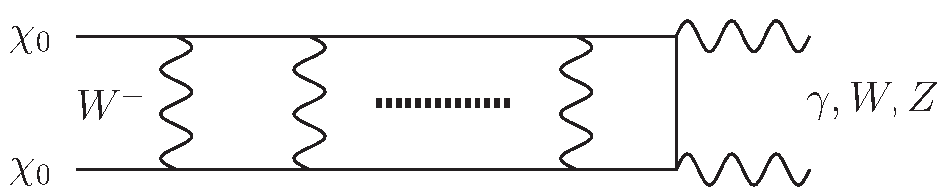
\includegraphics[width=0.7\hsize]{Sommerfeld.pdf}
  \caption{Ladder diagram contribution to the DM annihilation.}
  \label{fig:ladder}
\end{figure}

There remains a missing piece to describe the phenomenology of $\mathrm{TeV}$-scale DMs: the Sommerfeld enhancement effect \cite{Hisano:2004ds, Hisano:2006nn}.
This effect becomes important when the DM particles become non-relativistic like those in the current universe.
Consider the repeated exchange of electroweak gauge bosons between two initial DM particles before the annihilation as shown in Fig.~\ref{fig:ladder}, which is sometimes called a ladder diagram.
At a glance, the contribution of this diagram seems to be suppressed compared with the tree-level annihilation by a factor of $(\alpha/4\pi)^n$, where $\alpha \sim \alpha_1 \sim \alpha_2$ is a typical size of the coupling and $n$ is the number of gauge boson exchange.
However, when the initial particles are non-relativistic, it turns out that the proper power counting should be something like $(\alpha/\beta)^n$ instead of $\alpha^n$, where $\beta$ is the velocity of initial particles, observed in the center-of-mass system for simplicity.
This results in a possibly large contribution from ladder diagrams and we need to resum all of them to calculate the annihilation cross section accurately.
This effect affects both the thermal relic abundance of DM and the event rate at the indirect detection experiments, but the effect on the latter is typically larger since the average value of $\beta$ is smaller in the current universe than that at the freezeout temperature.

The resummation procedure can be performed by the use of the Bethe-Salpeter equation \cite{Salpeter:1951sz} as in \cite{Strassler:1990nw}.
Or equivalently, this effect can be seen as the deformation of the two-DM wave function from the plane wave according to the potential energy between them sourced by the electroweak interaction.
In this viewpoint, it is intuitive that the physics can be described by the Schr\"{o}dinger equation
\begin{align}
  \left[ - \frac{1}{m_\chi} \frac{d^2}{d r^2} + V(r) \right] \psi = E \psi,
\end{align}
where $\psi(r)$ is the s-wave part of the two-DM wave function, $r$ is the distance between two DMs, and $V(r)$ and $E = m_\chi \beta^2$ are the potential and kinetic energies of the two DM system, respectively.
Besides, we impose the outgoing boundary condition
\begin{align}
  \psi(r) \to e^{i p r} ~~ (r \to \infty),
\end{align}
with $p = m_\chi \beta$ being the DM momentum.
Remembering that the DM-DM interaction is local, the Sommerfeld enhancement factor $R$ that multiplies the tree-level cross section is given by $R = \left| \psi(\infty) / \psi(0) \right|^2$.
For example, when we consider the Coulomb potential $V(r) = -\alpha / r$, the equation can be analytically solved and we obtain
\begin{align}
  R = \frac{\pi \alpha / \beta}{1 - e^{- \pi \alpha / \beta}},
\end{align}
which causes a huge enhancement of the cross section when $\beta$ is small and $\alpha > 0$, or equivalently, the force between DMs is attractive.

The problem possesses an interesting feature when we consider a potential that is non-negligible only for a finite range such as the Yukawa potential for the electroweak interaction $V(r) = \alpha_2 e^{-m_W r} / r$.
In this case, when we neglect the small mass difference among an $SU(2)$ multiplet, the factor $R$ is strongly enhanced when the initial particle mass satisfies the equation
\begin{align}
  \sqrt{2} p_c = (2n - 1) \frac{\pi}{2}~~(n = 1, 2, \dots),
\end{align}
with $p_c \equiv \sqrt{2 \alpha_2 m_\chi / m_W}$.\footnote{
  If the mass difference $\delta m$ among an $SU(2)_L$ multiplet is comparable or larger than $\alpha_2 m_W$, the peaks move to the heavier direction.
  This may be the case for Higgsinos with a large mixing with gauginos.
}
Each choice of $n$ corresponds to a model point that has a bound state with zero binding energy and the enhancement is called the zero-energy resonance \cite{Landau1981Quantum}.
Note that the first peak with $n=1$ corresponds to $m_\chi \sim 2\,\mathrm{TeV}$, which is compatible with the assumption of the Wino DM or the MDM with the help of the non-thermal production.
Accordingly, as we will see from now, small regions around peaks of such models have already been excluded by the indirect detection experiments.

\begin{figure}[t]
  \centering
  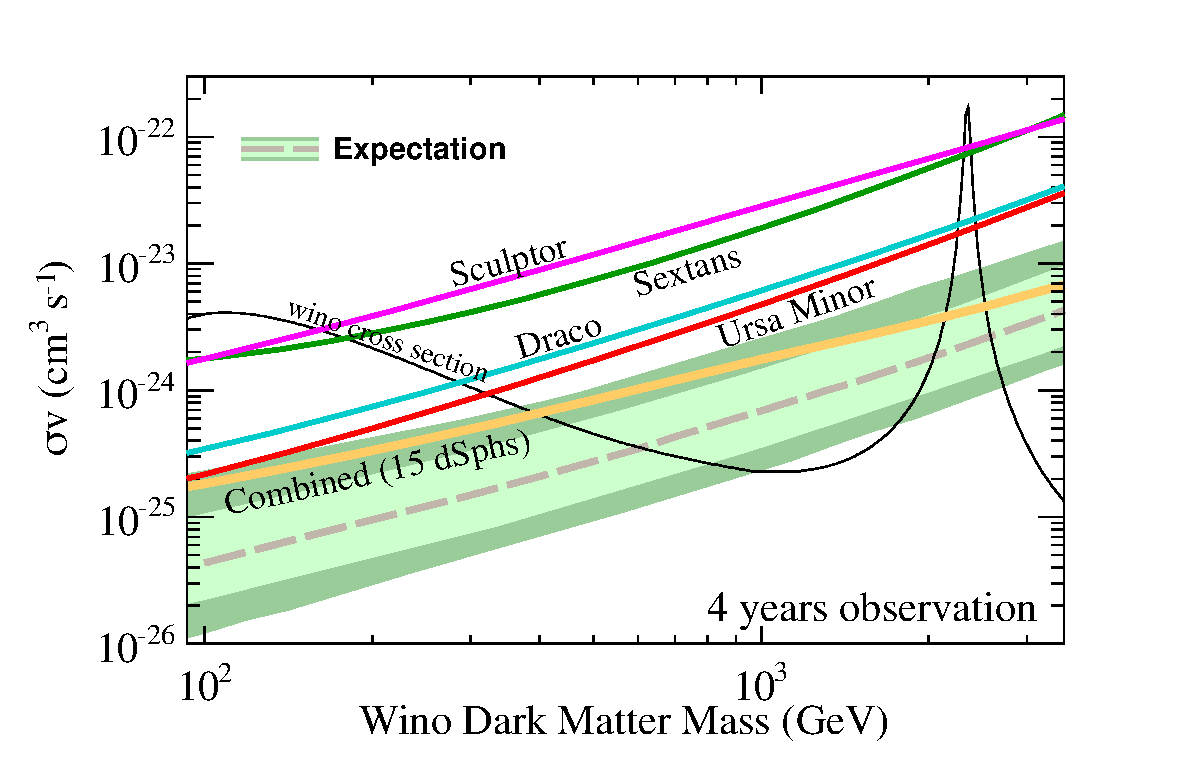
\includegraphics[width=0.6\hsize]{Present_limit.pdf}
  \caption{
    Constraint at the $95\,\%$ confidence level on the DM annihilation cross section taken from \cite{Bhattacherjee:2014dya}.
    The gray dotted line shows the combined result of $4$ years observation of $15$ dwarf galaxies by the Fermi-LAT collaboration, and the green bands show the observational errors.
    For the calculation of the constraint, the NFW profile is used.
    Also shown in the black solid line is the annihilation cross section of Wino.
  }
  \label{fig:indirect_current}
\end{figure}

There are many astrophysical observations that focus on several different particles or photons with different wavelengths.
Among them, the most stringent bound on DMs comes from the gamma-ray observations provided by several currently working or future planned collaborations such as the Fermi-LAT \cite{Atwood_2009}, GAMMA-400 \cite{GALPER2013297}, H.E.S.S. \cite{Abdallah:2016ygi}, and CTA \cite{Carr:2015hta}.
For Wino DM, for example, the annihilation mode into $W^{+} W^{-}$ dominates over the other modes and the photons emitted associated with the $W$-boson decay will be observed.
In Fig.~\ref{fig:indirect_current}, we show the constraint at the $95\,\%$ confidence level on the DM annihilation cross section, assuming $100\,\%$ branching ratio into $W^{+} W^{-}$ \cite{Bhattacherjee:2014dya}.
The gray dotted line shows the combined result of $4$-year observation of $15$ dwarf galaxies by the Fermi-LAT collaboration, while the black solid line denotes the annihilation cross section of Wino.
Note the existence of the zero-energy resonance at the position of $m_\chi \sim 2\,\mathrm{TeV}$ as estimated above.
From the figure, we can see that the parameter regions of Wino DM $m_\chi \lesssim 400\,\mathrm{GeV}$ and $m_\chi \sim 2\,\mathrm{TeV}$ are already excluded.\footnote{
  Currently, almost $10$-year observation data is expected to be accumulated and no sign of DM is reported.
  According to the estimation in \cite{Bhattacherjee:2014dya}, this may correspond to the exclusion of $m_\chi \lesssim 800\,\mathrm{GeV}$ and a slightly larger range around $m_\chi \sim 2\,\mathrm{TeV}$.
}

A similar analysis can be performed for other WIMP DM candidates.
The Higgsino is currently constrained only up to $350\,\mathrm{GeV}$ \cite{Krall:2017xij} due to the smallness of the annihilation cross section in particular for the heavier region.
For the MDM, 5-plet fermion is analyzed as an example in \cite{Abdalla:2018mve} and $m_\chi \lesssim 2\,\mathrm{TeV}$ and several narrow regions corresponding to the resonances are excluded.
As for the prospects of future experiments, firstly, an order of magnitude improvement on the constraint from that shown in Fig.~\ref{fig:indirect_current} is expected \cite{Bhattacherjee:2014dya} by a combination of the $15$-year observation at the Fermi-LAT and the $10$-year observation at the GAMMA-400, which covers most of the allowed parameter region of Wino DM.
Besides, the observation of the Galactic Center at the CTA collaboration will probe the relatively heavier region $m_\chi \sim \mathcal{O}(1)\, \mathrm{TeV}$ efficiently, reaching $\sigma v \sim \text{(a few)} \times 10^{-26}\, \mathrm{cm^3\, s^{-1}}$.
However, note that the observation of the Galactic Center is highly sensitive to the astrophysical uncertainties such as those on the $J$-factor.
Note also that the thermal Higgsino DM may be a challenging target of this kind of experiment even in the future, whose mass and cross section are $m_\chi \sim 1\,\mathrm{TeV}$ and $\sigma v < 10^{-26}\, \mathrm{cm^3\, s^{-1}}$, respectively.


%%%%%%%%%%%%%%%%%%%%%%%%%%%%%%%%%%%%%%%%%%%%%%%%%%%%%%%%%%%%%%%%%%%%%%%%%%%%%%%
\subsection{Concluding remarks}
\label{sec:summary_DM}
%%%%%%%%%%%%%%%%%%%%%%%%%%%%%%%%%%%%%%%%%%%%%%%%%%%%%%%%%%%%%%%%%%%%%%%%%%%%%%%

In this section, we have described the possibility of WIMPs to be the dominant component of DM.
We have seen that the $\mathrm{TeV}$-scale WIMPs with electroweak interactions can explain the DM relic abundance and studied two search methods of such WIMP DMs.
Both direct and indirect detection have strong powers to explore a large region of the WIMP mass.
However, it is revealed that the almost pure Higgsino will be difficult to probe because of its small scattering and annihilation cross section.
Besides, the constraints shown above assume the whole DM is composed of a WIMP and are also sensitive to the possibly large astrophysical uncertainties.
From the next section, we will see more robust ways of the WIMP search using collider experiments and consider whether we can probe the regions of the parameter space that are difficult to probe using DM search experiments.


% \bibliographystyle{elsarticle-num}
% \bibliography{../phd}

\end{document}


\clearpage

% Erase biblio in input file before turning on
\documentclass[12pt,twoside,book]{article}
\usepackage{docmute}

\input{../settings}

\begin{document}

%%%%%%%%%%%%%%%%%%%%%%%%%%%%%%%%%%%%%%%%%%%%%%%%%%%%%%%%%%%%%%%%%%%%%%%%%%%%%%%
\section{Direct collider search of WIMPs}
\setcounter{equation}{0}
%%%%%%%%%%%%%%%%%%%%%%%%%%%%%%%%%%%%%%%%%%%%%%%%%%%%%%%%%%%%%%%%%%%%%%%%%%%%%%%

\vskip 0.1in

In this section, we review the production of $\mathrm{TeV}$-scale WIMPs and search for their signals using the collider experiment.
In particular, we will summarize the current bounds for WIMPs obtained at the large hadron collider (LHC) and future bounds expected at the future planned $100\,\mathrm{TeV}$ colliders such as the hadron option of the future circular collider (FCC-hh) \cite{Benedikt:2651300} and the super proton-proton collider (SPPC) \cite{CEPC-SPPCStudyGroup:2015csa, CEPC-SPPCStudyGroup:2015esa}.
In Sec.~\ref{sec:wimp_production}, we discuss the dominant production processes of WIMPs at a hadron collider.
In Sec.~\ref{sec:disappearing_track} and \rem{???}, we review \rem{two???} different methods for the signal identification, the disappearing track search and mono-jet search \rem{???}, and summarize the current and future bounds.


%%%%%%%%%%%%%%%%%%%%%%%%%%%%%%%%%%%%%%%%%%%%%%%%%%%%%%%%%%%%%%%%%%%%%%%%%%%%%%%
\subsection{WIMP production}
\label{sec:wimp_production}
%%%%%%%%%%%%%%%%%%%%%%%%%%%%%%%%%%%%%%%%%%%%%%%%%%%%%%%%%%%%%%%%%%%%%%%%%%%%%%%

There are two relevant processes both of which significantly contribute to the WIMP production cross section.
The pair production via electroweak interaction is a universal process that can be considered for any WIMP considered in this thesis.
The decay of colored particles may also be efficient particularly for the MSSM.
In this subsection, we will review these two in order.


\subsubsection*{Pair production via electroweak interaction}

\begin{figure}[b]
  \centering
  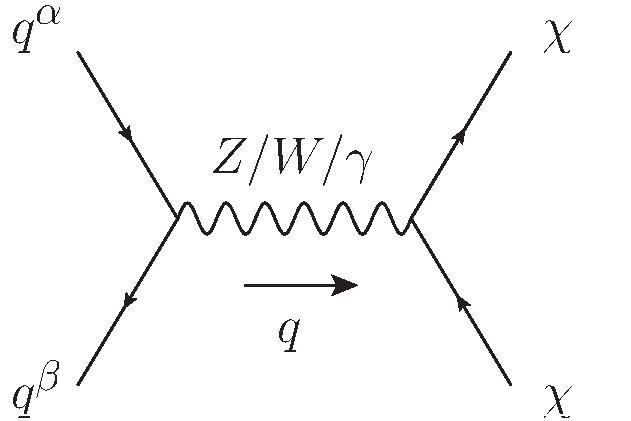
\includegraphics[width=0.4\hsize]{WIMP_production.pdf}
  \caption{WIMP pair production process at the hadron collider.}
  \label{fig:wimp_production}
\end{figure}

Since all the WIMPs considered here possess non-zero $SU(2)_L$ and $U(1)_Y$ charges, they can be directly produced via electroweak interaction at the hadron collider as shown in Fig.~\ref{fig:wimp_production}.
\footnote{
  All the Feynman diagrams in this thesis are drawn with the public code \texttt{JaxoDraw-2.1} \cite{BINOSI20091709}, which is a graphical user interface that allows users to draw Feynman diagrams intuitively and export them in the \texttt{eps} format with the help of the (modification of) \texttt{axodraw} style file for \LaTeX \cite{VERMASEREN199445}.
  Under the environment of macOS Mojave, it apparently fails to start, but one can still execute it by looking inside the application and start the Java executable file \texttt{jaxodraw-2.1-0.jar} directly.
  We would like to thank the authors for providing the best tools to write the thesis with.
  \rem{Where is the first place of Feynman diagrams?}
}
In the figure, $q^\alpha$ and $q^\beta$ denote the partons (namely, one of quarks or gluon) of the incident protons relevant for the process, while $\chi$ denotes the WIMP and $q$ is the momentum transfer.
Assuming the WIMP to be a $SU(2)_L$ $n$-plet with $U(1)_Y$ charge $Y$ and the mass $m_\chi$, this process is well described by the effective lagrangian
\footnote{
  In this subsection, we neglect the small mass difference among different components in the multiplet $\chi$ described in Sec.~\ref{sec:disappearing_track}.
  This approximation is valid since the mass difference is by far smaller than $m_\chi$ and has only a tiny effect on the production process.
}
\begin{align}
  \mathcal{L} &= \mathcal{L}_{\mathrm{SM}} + (D^\mu \chi)^\dagger (D_\mu \chi) - m_\chi^2 \chi^\dagger \chi &
  &\text{(complex scalar)}, \label{eq:lag_scalar}\\
  \mathcal{L} &= \mathcal{L}_{\mathrm{SM}} + \bar{\chi} (i \Slash{D} - m_\chi) \chi &
  &\text{(Dirac fermion)}, \label{eq:lag_fermion}
\end{align}
with $\mathcal{L}_{\mathrm{SM}}$ being the SM lagrangian, while the covariant derivative is given by
\begin{align}
  D_\mu \equiv \partial_\mu - i g_2 \Slash{W}^a T_n^a - i g_1 Y \Slash{B},
\end{align}
where $T_n^a$ ($a=1,2,3$) are $n$-dimensional representation matrices of $SU(2)_L$.
Note that when $\chi$ is a real scalar (Majorana fermion) with $Y=0$, the terms with $\chi$ in Eq.~\eqref{eq:lag_scalar} (Eq.~\eqref{eq:lag_fermion}) should be devided by two.

For the calculation, we neglect the effect of the electroweak symmetry breaking, which is valid because we are interested in the high-energy collision with the parton-level center-of-mass (CM) energy $\sqrt{s'} \equiv \sqrt{q^2} \gtrsim \mathrm{TeV}$.
Then, we consider the process in the CM frame and estimate the parton-level differential cross section as
\begin{align}
  \left. \frac{d \sigma_{\alpha \beta}}{d \sqrt{s'} d \Omega} \right|_{\text{CM}}
  &= \frac{C_{\alpha \beta}}{8 s'} \left( 1 - \frac{4 m_\chi^2}{s'} \right)^{3/2} \sin^2 \theta
  & &(\text{complex scalar}) \label{eq:parton_cross_section_scalar} \\
  \left. \frac{d \sigma_{\alpha \beta}}{d \sqrt{s'} d \Omega} \right|_{\text{CM}}
  &= \frac{C_{\alpha \beta}}{4 s'} \sqrt{1 - \frac{4 m_\chi^2}{s'}}
  \left[ 1 + \frac{4 m_\chi^2}{s'} + \left( 1 - \frac{4 m_\chi^2}{s'} \right) \cos^2 \theta \right]
  & &(\text{Dirac fermion}), \label{eq:parton_cross_section_fermion}
\end{align}
where $\theta$ is the angle between the momentum of the initial parton $q_a$ and that of one of the final state WIMPs.
These expressions are valid only when the center of mass energy exceeds the production threshold, $\sqrt{s'} > 2m_\chi$.
Note also that these expressions represent inclusive cross sections, \textit{i.e.}, the total cross section for the production of any component of the WIMP multiplet $\chi$.
The coefficient $C_{\alpha \beta}$ consists of contributions from $U(1)_Y$ and $SU(2)_L$ gauge bosons,
\footnote{
  There is no contribution from the interference term between $U(1)_Y$ and $SU(2)_L$ contributions, since it is proportional to $\mathrm{Tr} (T^a_n) = 0$.
}
\begin{align}
  C_{\alpha \beta} = c_{1 \alpha \beta} Y^2 \alpha_1^2
  + c_{2 \alpha \beta} I(n) \alpha_2^2,
\end{align}
with $I(n)$ being the Dynkin index for the $n$-dimensional representation given by
\begin{align}
  I(n) \equiv \frac{n^3-n}{12},
  \label{eq:dynkin}
\end{align}
which is normalized so that $I(2) = 1/2$.
The explicit form of $c_{1 \alpha \beta}$ and $c_{2 \alpha \beta}$, which are sizes of the couplings between partons of our choice and gauge bosons, can be expressed using the $U(1)_Y$ charge for a parton $Y_\alpha$ and the $SU(2)_L$ reducible 13-dimensional representation matrices for partons $T^a_{\alpha \beta}$ as
\begin{align}
  c_{1 \alpha \beta} &= Y_\alpha^2 \delta_{\alpha \beta},\\
  c_{2 \alpha \beta} &= \sum_a \left| T^a_{\alpha \beta} \right|^2.
\end{align}
Recalling that $\alpha_1 < \alpha_2$ and that we often consider the WIMPs with large $n$ and moderate $Y$, the WIMP production cross section grows as $n^3$ for larger multiplets according to Eq.~\eqref{eq:dynkin}.

In the reality, the initial state of the hadron collider is not the individual partons but two protons.
To obtain the cross section for the two protons initial state, we rely on the parton distribution function (PDF), which expresses the fraction of the partons with some given momentum in each accelerated proton.
Let $f_a (x)$ ($0 < x < 1$) be the PDF for a given parton $a$ inside a proton with momentum $p^\mu$.
$f_a (x)$ can be interpreted as a probability distribution to find the parton $\alpha$ with momentum $x p^\mu$, so we have a relationship
\begin{align}
  \sum_\alpha \int_0^1 dx \, x f_\alpha (x) = 1,
\end{align}
associated with the total momentum conservation, and
\begin{align}
  \int_0^1 dx \, \left[ f_d (x) - f_{\bar{d}} (x) \right] &= 1,\\
  \int_0^1 dx \, \left[ f_u (x) - f_{\bar{u}} (x) \right] &= 2,
\end{align}
from the composition of the proton.
Using the PDF, the cross section for the process of interest at the hadron collider is evaluated as
\begin{align}
  \frac{d \sigma}{d \sqrt{s'} d \Omega} =
  \sum_{\alpha, \beta} \int_0^1 dx_1 dx_2 \, f_\alpha (x_1) f_\beta (x_2) \delta \left( s' - s x_1 x_2 \right)
  \left. \frac{d \sigma_{\alpha \beta}}{d \Omega} \right|_{\text{lab}},
\end{align}
where $\sqrt{s}$ is the CM energy of the proton-proton collision.
Note that the cross section in the integrand is a function of $x_1$ and $x_2$, which is obtained by performing the appropriate Lorentz transformation to $\left. d \sigma_{\alpha \beta} / d \Omega\, \right|_{\text{CM}}$.
\rem{Comment on factorization scale?}

\begin{figure}[t]
  \centering
  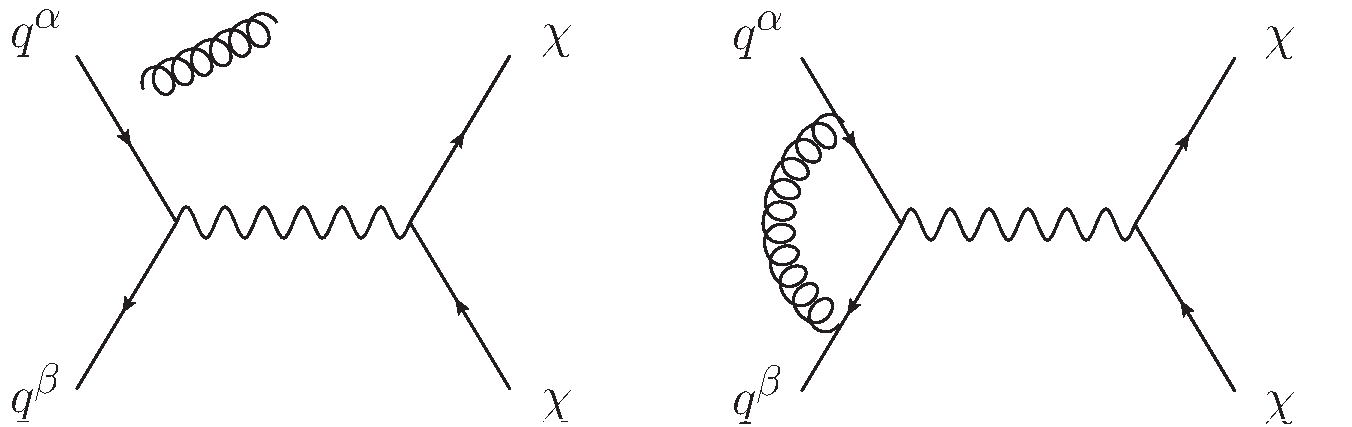
\includegraphics[width=0.8\hsize]{WIMP_production_NLO.pdf}
  \caption{Example of NLO QCD contributions to the WIMP pair production process.}
  \label{fig:WIMP_production_NLO}
\end{figure}

Hadron colliders have several more features related to the strong interaction of quantum chromodynamics (QCD).
Firstly, the next-to-leading order (NLO) QCD contribution to each process is not necessarily negligible.
For the WIMP pair production, the real and virtual emission of a gluon shown in the left and right panels of Fig.~\ref{fig:WIMP_production_NLO}, respectively, give the NLO QCD contributions, which will also be taken into account from now on.
In particular, when the large transverse momentum is important for the phenomenology of our concern, such as the case in Sec.~\rem{???}, the real emission of a gluon with sizable transverse momentum significantly modifies the calculation.
Secondly, all the colored particles in the initial, intermediate, and final states should be accompanied with numbers of soft emissions of gluons, which is the phenomena so-called the parton shower.
In practice, there is a difficulty caused by the partial overlap of the gluon phase space between the one-gluon emission cross section considered as an NLO QCD effect and the same considered as the parton shower.
To avoid this overlap, we often perform the matching procedure, in which we set some merging energy scale by hand and include the contribution to the cross section with gluon energy above (below) the scale only from the NLO QCD (parton shower) calculation.
Finally, the colored particles in the final states should eventually be confined, which is called the hadronization, and observed as some energetic and collimated sprays of hadrons, which as a whole is called jets.

In the following, we perform the numerical calculation, taking account of all the above complexities.
For this purpose, we make use of the Monte Carlo generator \texttt{MadGraph5 aMC@NLO (v2.6.3.2)} \cite{Alwall:2011uj,Alwall:2014hca} with the successive use of \texttt{Pythia8} \cite{Sjostrand:2014zea} for the parton shower, hadronization, and matching and \texttt{Delphes (v3.4.1)} \cite{deFavereau:2013fsa} for the detector simulation, including the definition of jets as observed objects.
We use the so-called MLM-style matching \cite{Mangano:2006rw} with the merging scale of $67.5\,\mathrm{GeV}$ and \texttt{NNPDF2.3QED} with $\alpha_3 (M_Z) = 0.118$ \cite{Ball:2013hta} as a canonical set of PDFs.
% For the renormalization and factorization scales, we adopt the default values of MadGraph5 aMC@NLO, \textit{i.e.}, the central $m^2_T$ scale after $k_T$-clustering of the event.

\begin{table}[t]
  \centering
  \begin{tabular}{c|cccc}
    WIMP name & Higgsino & Wino & $5$-plet Majorana fermion & $5$-plet real scalar \\ \hline
    $\sigma_{\mathrm{LO}}$ $[\mathrm{fb}]$ & 15 & 52 & \rem{???} & \rem{???} \\
    $\sigma_{\mathrm{NLO}}$ $[\mathrm{fb}]$ & 17 & 60 & \rem{???} & \rem{???} \\ \hline
    $K$-factor & 1.15 & 1.15 & &
  \end{tabular}
  \caption{
    Table of pair production cross sections of several types of WIMPs.
    The CM energy $\sqrt{s} = 100\,\mathrm{TeV}$ is assumed and WIMP masses are set to be $1\,\mathrm{TeV}$.
  }
  \label{tab:cross_section_WIMPs}
\end{table}

In Table~\ref{tab:cross_section_WIMPs}, we list the production cross sections of various WIMPs via a weak gauge boson exchange at a $\sqrt{s} = 100\,\mathrm{TeV}$ hadron collider.
As for the WIMP mass, we use the common value $m = 1\,\mathrm{TeV}$ to compare the cross sections among different choice of quantum numbers.
$\sigma_{\mathrm{LO}}$ and $\sigma_{\mathrm{NLO}}$ denote the production cross sections without and with the NLO QCD correction, respectively, while the last line is the so-called $K$-factor defined as $K = \sigma_{\mathrm{NLO}} / \sigma_{\mathrm{LO}}$.
From the table, by paying attention to the factor two difference in degrees of freedom between the Dirac (Higgsino) and Majorana (Wino and $5$-plet) fermions, we can roughly see the dependence of the cross section on the $SU(2)_L$ charge $\sigma \propto n^3$.
\rem{Cross section to neutral Higgsino seems missing}

\begin{table}[t]
  \centering
  \begin{tabular}{c|cccc}
    Wino mass $\mathrm{[TeV]}$ & 1.0 & 1.5 & 2.0 & 2.9 \\ \hline
    $\sigma_{\mathrm{LO}}$ $[\mathrm{fb}]$ & 52 & 12 & 4.0 & 0.86\\
    $\sigma_{\mathrm{NLO}}$ $[\mathrm{fb}]$ & 60 & 15 & 4.7 & 1.0 \\ \hline
    $K$-factor & 1.15 & 1.20 & 1.19 & 1.21
  \end{tabular}
  \caption{
    Table of pair production cross sections of Wino with several choice of masses.
    The CM energy $\sqrt{s} = 100\,\mathrm{TeV}$ is assumed.
  }
  \label{tab:cross_section_Wino_mass}
\end{table}

In Table \ref{tab:cross_section_Wino_mass}, we also show the mass dependence of the Wino pair production cross section.
For heavier mass, wider range of $\sqrt{s'}$ is below the production threshold $2 m_{\chi}$ or accompanied with a small suppression factor $(1-4 m_\chi^2 / s')^{1/2}$ as shown in Eq.~\eqref{eq:parton_cross_section_fermion}, and the cross section becomes significantly smaller.
However, values in the tables still denote that plenty of well-motivated WIMP DM candidates, such as $1\,\mathrm{TeV}$ Higgsino and $2.9\,\mathrm{TeV}$ Wino, are produced at, for example, the $30\,\mathrm{ab}^{-1}$ option of the FCC-hh.

\begin{figure}[t]
  \centering
  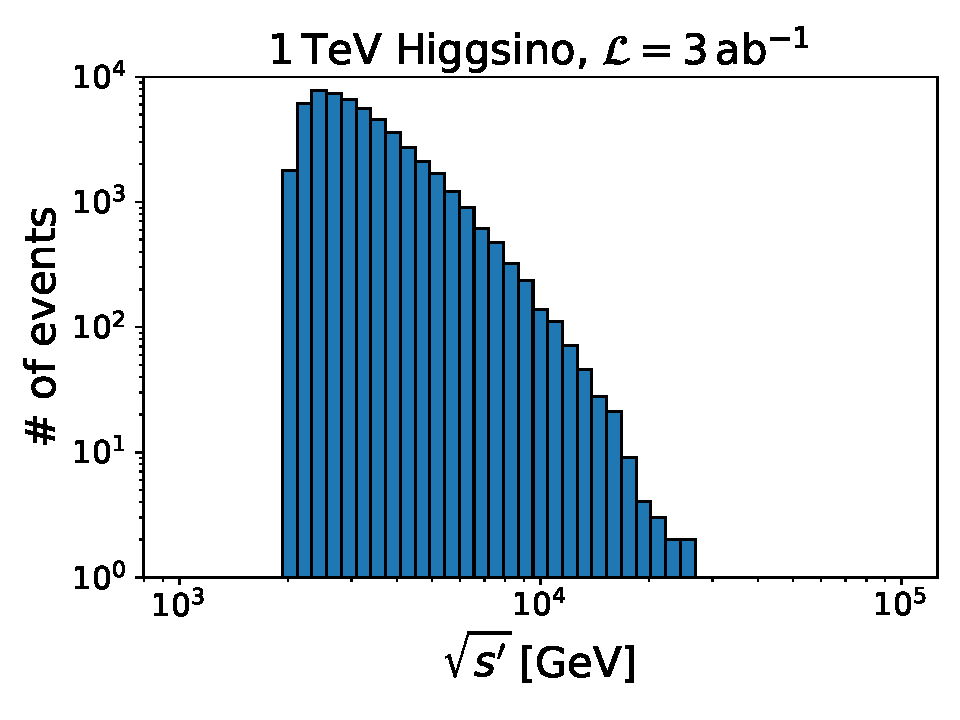
\includegraphics[width=0.48\hsize]{invariant_mass_Higgsino.pdf}
  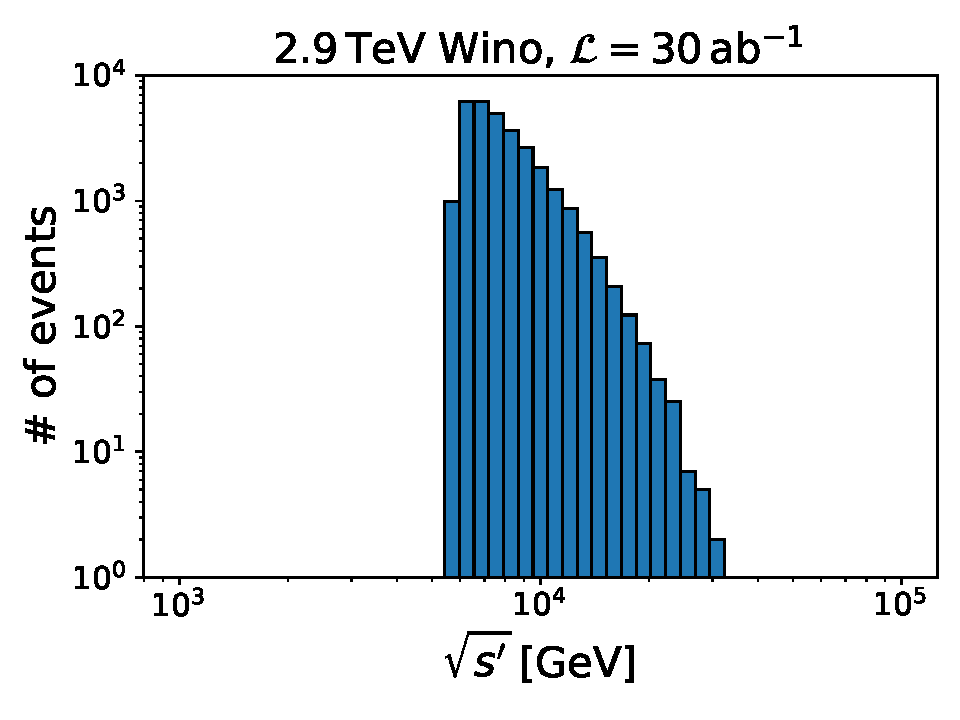
\includegraphics[width=0.48\hsize]{invariant_mass_Wino.pdf}
  \caption{
    Histogram of the $\sqrt{s'}$ distribution for $\sqrt{s} = 100\,\mathrm{TeV}$.
    \textit{Left:} Production of $1\,\mathrm{TeV}$ Higgsino at $\mathcal{L} = 3\,\mathrm{ab}^{-1}$.
    \textit{Right:} Production of $2.9\,\mathrm{TeV}$ Wino at $\mathcal{L} = 30\,\mathrm{ab}^{-1}$.}
  \label{fig:invariant_mass}
\end{figure}

In Fig.~\ref{fig:invariant_mass}, we show the $\sqrt{s'}$ distribution for the pair production process at a $\sqrt{s} = 100\,\mathrm{TeV}$ collider.
Left and right figures correspond to the production of $m_\chi = 1\,\mathrm{TeV}$ Higgsino at the integrated luminosity $\mathcal{L} = 3\,\mathrm{ab}^{-1}$ and of $m_\chi = 3\,\mathrm{TeV}$ Wino at $\mathcal{L} = 30\,\mathrm{ab}^{-1}$, respectively.
At around $\sqrt{s'} \sim 2 m_\chi$, we clearly see the production threshold and the suppression effect $\sigma \propto (1-4 m_\chi^2 / s')^{1/2}$.
On the other hand, when $\sqrt{s'}$ becomes much larger than $2m_\chi$, we can see the correct behavior of the cross section, which decreses as $\sigma \propto (\sqrt{s'})^{-3}$ as Eq.~\eqref{eq:parton_cross_section_fermion} indicates.
Note that these properties are universal among several processes, including the dominant contribution \rem{Correct?} to the gluino pair production through the $s$-channel gluon exchange disscused in the next subsection, and the lepton pair production through via an electroweak gauge boson that is the main topics in Sec.~\rem{???}.

\rem{Histogram of angular dependence}

\rem{Is angular dependence affected by the Lorentz boost?}


\subsubsection*{Decay of colored particles}

In hadron colliders, particles with color charges have far more chance to be produced than non-colored particles.
When we consider the split SUSY or the anomaly mediation model reviewed in Sec.~\ref{sec:MSSM}, gluino tends to be relatively light, whose decay produces WIMPs.
Without fine-tuning of Higgsino and gaugino masses, gluino lifetime is sufficiently short and only its decay products are observed by the detectors.
Since all the SUSY particles finally decay into the LSP as described in Sec.~\ref{sec:MSSM}, the gluino production cross section can effectively be counted as the production cross section of WIMPs in these models.

\begin{table}[t]
  \centering
  \begin{tabular}{c|ccc}
    gluino mass $\mathrm{[TeV]}$ & 6.0 & 7.0 & 8.0 \\ \hline
    $\sigma(p p \to \tilde{g} \tilde{g})\, \mathrm{[fb]}$ & 7.9 & 2.7 & 1.0
  \end{tabular}
  \caption{Gluino pair production cross section at $\sqrt{s} = 100\,\mathrm{TeV}$.}
  \label{tab:gluino_pair}
\end{table}

Keeping the R-parity conservation in our mind, the dominant process accompanied with gluinos in these models is the gluino pair production.
In Table \ref{tab:gluino_pair}, we summarize the gluino pair production cross section for various gluino masses at $\sqrt{s} = 100\,\mathrm{TeV}$, taken from \cite{Asai:2019wst}.
The calculation is again performed using \texttt{MadGraph5 aMC@NLO} and only the LO QCD processes are considered.
The values in the table show that the gluino pair production process, dependeing on its mass, may give much larger cross section for the WIMP production than the purely electroweak processes described above.

\rem{Comment on AMSB $m_{3/2}$ and $L$ for the table?}


%%%%%%%%%%%%%%%%%%%%%%%%%%%%%%%%%%%%%%%%%%%%%%%%%%%%%%%%%%%%%%%%%%%%%%%%%%%%%%%
\subsection{Disappearing track search}
\label{sec:disappearing_track}
%%%%%%%%%%%%%%%%%%%%%%%%%%%%%%%%%%%%%%%%%%%%%%%%%%%%%%%%%%%%%%%%%%%%%%%%%%%%%%%

In the last section, we have checked the possibility that a large number of WIMPs are produced at hadron colliders.
On the other hand, the detection of produced WIMPs is not a straight-forward task, because there are huge background events with many charged and/or colored particles.
To reduce the background events and obtain the best possible reach for WIMPs, we consider several methods using typical properties for the WIMP signals, one of which is the disappering track signal described here.

As also mentioned in Sec.~\rem{DM??}, the spontaneous breaking of the electroweak symmetry leads to the mass splitting among an $SU(2)_L$ multiplet, leaving the charge neutral component as the lightest one.
As a result, the charged components of a multiplet, if produced, are unstable and eventually decay into the neutral component.
However, the mass splitting is so small in many cases that the typical flight length of the charged components is comparable to the detector size.
Such long-lived charged particles, which travel for a few $\mathrm{cm}$ and then decay into an invisible counterpart, can be detected as charged tracks disappearing at the middle.
They are very characteristic signals and can be used as the most efficient discriminator between the SM background and the WIMP signals.
In this section, we will describe what we have summarized above in more detail.


\subsubsection*{Mass splitting among an $SU(2)_L$ multiplet}

First, we consider the mass splitting caused by the spontaneous breakdown of the electroweak symmetry.
In particular, we start with the tree-level propagation of heavy particles, such as the SUSY particles other than the LSP, or another unknown particles.
After integrating out all the heavy particles other than the SM particles and the light WIMP, we may obtain operators of the form of $\mathcal{O} = M_{i j} \chi_i \chi_j$, where $\chi$ denotes the WIMP and $i$ is the $SU(2)_L$ index.
This operator causes the mass splitting only when $M_{i j}$ transforms non-trivially under the $SU(2)_L$ symmetry.
Then, we can explicitlly construct the lowest dimensional operator among those relevant for the mass splitting.
For Higgsino,
\begin{align}
  \mathcal{O} = \frac{1}{\Lambda} (\bar{\chi} H^{*}) (H \chi),
  \label{eq:Higgsino_mass_splitting}
\end{align}
where $\chi = (\tilde{H}_u, -i \sigma_2 \tilde{H}_d^{*})^t$, $\Phi$ is the SM Higgs doublet with $Y = 1/2$, $\Lambda$ is the cut-off scale of the effective theory, \textit{i.e.}, the typical mass scale of the relevant heavy particles, and the parenthesis denotes the $SU(2)_L$ invariant product of fundamental representations.
Similarly, for Wino, \cite{Gherghetta:1999sw}
\begin{align}
  \mathcal{O} = \frac{1}{\Lambda^3} (H^\dagger \sigma^a H) (H^\dagger \sigma^b H) \tilde{W}^a \tilde{W}^b,
  \label{eq:Wino_mass_splitting}
\end{align}
A simple implication of this observation is that, for multiplets with large $n$, there are suppression factors that keep the tree-level mass splitting small.
For Wino, the suppression is of $\mathcal{O} (M_W^4 / \Lambda^3)$, which yields a splitting smaller than $10\,\mathrm{MeV}$ for heavy paritlces with a few $\mathrm{TeV}$ masses.
For fermionic MDMs with $n \gtrsim 5$, a similarly small mass splitting at the tree-level is expected.
\footnote{
  For scalar MDMs, there is another renormalizable operator that generates a mass splitting
  \begin{align*}
    \mathcal{O} = - \lambda_H \left( \chi^{*} \sigma^a \chi \right) \left( H^\dagger \sigma^a H \right).
  \end{align*}
  Unless $\lambda_H$ is sufficiently small, the disappearing track search cannot be applied because of the too large mass splitting.
}
This is the main reason why the loop correction plays more important role for the mass splitting of Wino and MDMs.

The situation is different for Higgsino because of the much less drastic suppression factor of $\mathcal{O} (M_W^2 / \Lambda)$, which generates $\mathcal{O} (100)\,\mathrm{MeV}$ mass splitting for $\Lambda \lesssim \mathrm{10}\,\mathrm{TeV}$.
\footnote{
  For the order estimation of the mass splitting, we have taken account of the size of the coupling constants omitted in Eq.~\eqref{eq:Higgsino_mass_splitting}, using the rough estimation $g_1^2 \sim g_2^2 \sim 1/10$.
}
In fact, in models like the split SUSY, the mixing between Higgsino and heavier gauginos can generate the large mass splitting among the Higgsino components.
As a result, neutral components that originally forms a Dirac fermion splits into two Majorana fermions with mass difference $\Delta m_0$, and the charged components also become heavier than the lighter neutral component by $\Delta m_{+}^{\mathrm{(tree)}}$.
According to \cite{Fukuda:2017jmk}, their approximate expressions are given by
\begin{align}
  \Delta m_0 &\simeq \frac{M_W^2}{g_2^2} \left( \frac{g_1^2}{M_1} + \frac{g_2^2}{M_2} \right),\\
  \Delta m_{+}^{\mathrm{(tree)}} &\simeq \frac{M_W^2}{2 g_2^2} \left[
  \left( \frac{g_1^2}{M_1} + \frac{g_2^2}{M_2} \right)
  + \mathrm{sgn} (\mu) \sin 2\beta \left( \frac{g_1^2}{M_1} - \frac{g_2^2}{M_2} \right) \right],
  \label{eq:Higgsino_delm_tree}
\end{align}
assuming the CP invariance for simplicity.
Note that the results agrees with the previous order estimation with $\Lambda \sim M_1$, $M_2$.

Next we consider the loop correction to the WIMP masses.
When the loop is composed of heavy particles, the effective operator that causes the mass splitting again becomes the same as above, which is now associated with a small loop factor.
Thus, the largest contribution comes from the gauge boson - WIMP loop.
For the charged componets of Higgsino, the one-loop result is known: \cite{Fukuda:2017jmk}
\begin{align}
  \Delta m_{+}^{\mathrm{(rad)}} \simeq \frac{1}{2} \alpha_2 M_Z \sin^2 \theta_W
  \left( 1 - \frac{3 M_Z}{2\pi m_\chi} \right)
  \sim 355\,\mathrm{MeV} \left( 1 - \frac{3 M_Z}{2\pi m_\chi} \right),
  \label{eq:Higgsino_delm_rad}
\end{align}
with $\theta_W$ being the Weinberg angle, which gives $\Delta m_{+}^{\mathrm{(rad)}} \simeq 341\,\mathrm{MeV}$ for $m_\chi = 1.1\,\mathrm{TeV}$ and may be comparable to $\Delta m_{+}^{\mathrm{(tree)}}$.
On the other hand, for Wino, we have the two-loop result \cite{Ibe:2012sx}
\newcommand{\logmchi}{\left( \log \frac{m_\chi}{\mathrm{GeV}} \right)}
\begin{align}
  \frac{\Delta m}{\mathrm{MeV}} =
  &-413.315 + 305.383 \logmchi - 60.8831 \logmchi^2\\
  &+ 5.41948 \logmchi^3 - 0.181509 \logmchi^4,
\end{align}
which exhibits $\Delta m \simeq 165\,\mathrm{MeV}$ for $m_\chi = 2.9\,\mathrm{TeV}$.
For the MDM, there are neutral, singly charged, doubly charged, and so on, components.
Among them, the neutral and singly charged components have the smallest mass difference of $\Delta m \simeq 166\, \mathrm{MeV}$ \cite{Cirelli:2005uq}, which is the most important value for the collider search.


\subsubsection*{Lifetime of charged components}

Small mass difference of a WIMP allows the heavier charged component to decay into the neutral component and SM particles via a off-shell $W$ boson.
Depending on the size of the relevant mass difference $\Delta m$, there are several channels that contributes to the decay \cite{Chen:1995yu}.
For tiny $\Delta m < m_\pi$ with $m_\pi$ being the charged pion mass, $\chi^{+} \to \ell^{+} \nu_\ell \chi^0$ ($\ell = e, \mu$) are the unique decay modes.
Once $\Delta m$ exceeds $m_\pi$, the mode $\chi^{+} \to \pi^{+} \chi^0$ opens up and becomes the dominant one.
After $\Delta m \gtrsim 1\, \mathrm{GeV}$, final states with two and three pions start to give a sizable contribution, and the total decay rate asymptotes to that for $\chi^{+} \to q' \bar{q} \chi^0$.
For larger mass difference, the mode $\chi^{+} \to \tau^{+} \nu_\tau \chi^0$ may also be allowed.
As a whole, these decay modes determine the lifetime of a WIMP, which is typically long enough to be probed by experiments thanks to the small mass difference.

Let $\tau$ be the lifetime of the (singly) charged component of a WIMP, defined using the total decay rate $\Gamma$ as $\tau \equiv 1/\Gamma$.
Taking into account that a WIMP, if created at colliders with sufficiently high collision energy, has a velocity comparable to the speed of light $c$, $c \tau$ expresses the rough estimation of its flight length inside detectors.
For Higgsino with $m_\pi < \Delta m \lesssim 1\,\mathrm{GeV}$,
\footnote{
  We are not interested in Higgsino with $\Delta m \gtrsim 1\, \mathrm{GeV}$ here, since the corresponding flight length will be much shorter than $\mathcal{O} (1)\, \mathrm{cm}$, which is the scale of the detectors.
}
we can estimate \cite{Chen:1995yu,Thomas:1998wy}
\begin{align}
  c \tau \simeq 0.7\, \mathrm{cm}
  \left[ \left( \frac{\Delta m_{+}}{340\,\mathrm{MeV}} \right)^3
  \sqrt{1 - \frac{m_\pi^2}{\Delta m_{+}^2}} \right]^{-1},
\end{align}
where $\Delta m_{+} \equiv \Delta m_{+}^{\mathrm{tree}} + \Delta m_{+}^{\mathrm{rad}}$ with using Eqs.~\eqref{eq:Higgsino_delm_tree} and \eqref{eq:Higgsino_delm_rad}.
Since the mass difference for wino is a factor two smaller than Higgsino, we obtain a much longer flight length
\begin{align}
  c \tau \simeq 3.1\, \mathrm{cm} \left[
  \left( \frac{\Delta m}{165\, \mathrm{MeV}} \right)^3
  \sqrt{1 - \frac{m_\pi^2}{\Delta m^2}} \right]^{-1},
\end{align}
which gives $c\tau \simeq 5.8\,\mathrm{cm}$ for $\Delta m = 165\,\mathrm{MeV}$.
The same calculation applies to the MDMs with $n \geq 5$ and $\Delta m = 166\, \mathrm{MeV}$, resulting in somewhat shorter flight length that scales as $c \tau \sim 44\, \mathrm{cm} / (n^2 - 1)$ \cite{Cirelli:2005uq} due to the stronger interaction with $W$ bosons.
\rem{Scalar?}


\subsubsection*{Disappering track signal}

Once a long-lived charged component of WIMP is produced, it is detected by the trackers installed in the innermost part of the detectors for the case of ATLAS and CMS collaborations at the LHC.
For example, in the ATLAS setup, several tracking detectors are equipped cyrindrically around the beam line from the radius $r = 3\,\mathrm{cm}$ to $108\,\mathrm{cm}$.
The pixel detector spans the radius from $3\,\mathrm{cm}$ to $12\,\mathrm{cm}$, the strip semiconductor tracker (SCT) from $30\,\mathrm{cm}$ to $52\,\mathrm{cm}$, and the transition radiation tracker from $56\,\mathrm{cm}$ to $108\,\mathrm{cm}$.
In particular, pixel detectors are the most important for our discussion, which are composed of four layers, with the innermost one being the rescently equipped so-called the insertable B-layer \cite{Capeans:1291633, CERN-LHCC-2012-009, Abbott:2018ikt}.
To detect the charged track signal of a long-lived WIMP with the typical flight length of $\mathcal{O} (1)\, \mathrm{cm}$, they require the hit at every layer of the pixel detector and apply the SCT veto to search for the track signal disappearing in between $12\,\mathrm{cm} < r < 30\,\mathrm{cm}$.
As for the fake events within the SM, the SCT veto denies the possibility for a stable SM particle to mimic the signal.
However, there are two important sources of the fake track generated by hadrons/electrons and the so-called pile-up.

The first possibility with hadrons/electrons is a physical background caused by the interaction of hadrons with detector material or by the hard photon emission of electrons.
After these interactions, the orbit of a hadron/electron is bended and, if this secondary interaction point is between the pixel trackers and the SCT, two tracks in these two detectors are not identified with each other.
As a result, the first track in the pixel trackers seems to disappear in the middle, which mimics the true WIMP signals.
In the LHC, this type of background dominates and generates $\mathcal{O}(10$--$100)$ fake tracks for $\sqrt{s}=13\,\mathrm{TeV}$, $\mathcal{L} = 36.1\,\mathrm{fb}^{-1}$ (see Fig.~7 of \cite{Aaboud:2017mpt}).

On the other hand, for future hadron colliders, the second possibility of the fake track from the pile-up may be more and more important.
In hadron colliders, a bunch of protons are accelerated at the same time and two bunches ``collide'' with each other with some given frequency.
Since there are many protons inside a bunch, typically more than one collisions of two protons occur for each bunch crossing.
The average number of collisions per bunch crossing is often denoted as $\Braket{\mu}$ and the values of $\Braket{\mu} \sim 20$, $80$, and $200$ are expected for LHC Run-2, Run-3, and HL-LHC.
With this many collisions, there are a lot of collision products detected almost at the same time, which makes the signal significantly messy.
Then, among a huge number of hits on track detectros, several of them occasionally form a straight line in position and time, which is sometimes called the fake track.
Since this track is only a fake, it can easily pass the SCT veto and mimic the disappearing track signal of WIMPs.
In the real experiment, the rate for fake track reduces as we require more hits on trackers.
See the results below for a concrete estimation of the fake track rate at the FCC-hh.

\begin{figure}[t]
  \centering
  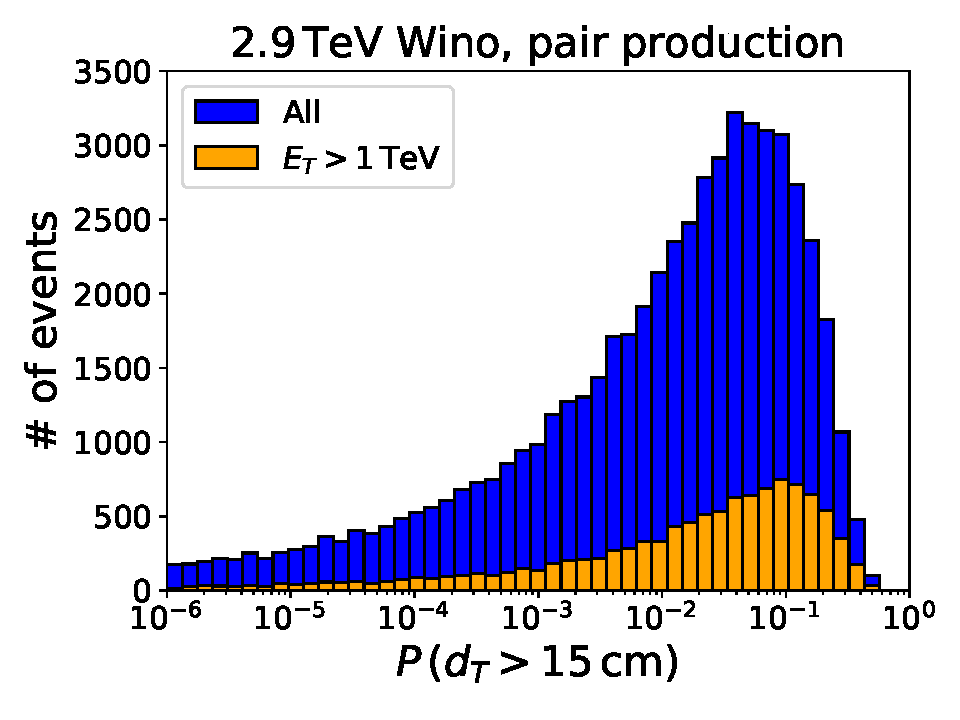
\includegraphics[width=0.5\hsize]{survival_probability.pdf}
  \caption{
    Distribution of the survival probability $P(d_T > 15\,\mathrm{cm})$ for $2.9\,\mathrm{TeV}$ Wino.
    The pair prodction process at $\sqrt{s}=100\,\mathrm{TeV}$ and $\mathcal{L} = 30\,\mathrm{ab}^{-1}$ is assumed.}
  \label{fig:survival_probability}
\end{figure}

From now on, we estimate how many events are expected at the FCC-hh.
Recalling that the detectors are installed in a cyrindrical geometry, the transverse distance $d_T$ of the WIMP flight measured from the beam line plays an important roll.
We can estimate the probability for $d_T$ to be larger than $d$ as
\begin{align}
  P(d_T > d) = \exp \left( -\frac{d}{\beta \gamma c \tau \sin\theta} \right),
  \label{eq:survival_probability}
\end{align}
where $\beta$ is the WIMP velocity, $\gamma \equiv (1-\beta^2)^{-1/2}$, and $\theta$ is the angle between the WIMP momentum and the beam line.
One of the implications of the above expression is that WIMPs with large transverse momentum have larger possibility to survive for a long time.
This enlarges the importance of considering the NLO (and higher order) QCD processes with real emission for the pair production.
Due to the hard emission of gluon, the produced pair of WIMPs is recoiled in an opposite direction, and WIMPs tend to have larger transverse momentum than the case without gluon emission.
It can be directly checked that, for $\sqrt{s}=100\,\mathrm{TeV}$, even the two-gluon emission process possesses non-negligible contribution to the simulation of the disappearing track search for WIMPs.

In Fig.~\ref{fig:survival_probability}, we show the distribution of $P(d_T > 15\,\mathrm{cm})$ (which is motivated by the FCC-hh detector setup assumed below) for the $2.9\,\mathrm{TeV}$ Wino, $\sqrt{s} = 100\,\mathrm{TeV}$, and $\mathcal{L} = 30\,\mathrm{ab}^{-1}$.
Here, we only consider the WIMP pair production process with upto one gluon emission as an example.
Note that $\tau \simeq 5.8\,\mathrm{cm}$ for this setup.
We can see that the increase in the probability by $\gamma$ and the decrease by $\beta$ and $\sin\theta$ roughly cancels with each other on average, resulting in a peak of the distribution at $P \sim 10^{-1} \sim \exp (-15\,\mathrm{cm} / \tau)$.
By summing the shown probabilities for all produced winos, we can obtain the expectation value $N_{15}$ for the number of winos with $d_T > 15\,\mathrm{cm}$.
We find $N_{15} \sim 2400$,
\footnote{
  In the real analysis, it may also be important to put a cut on the missing transverse energy $\Slash{E}_T$ to further reduce the number of background.
  If we require $\Slash{E}_T > 1\,\mathrm{TeV}$ as \cite{Asai:2019wst}, we expect smaller number of winos $N_{15} \sim 600$.
}
to which a lot of winos around and above the peak position $P \sim 10^{-1}$ significantly contribute.
Thus, we infer that we can detect the wino signal if we can suppress the number of background events to $\lesssim \mathcal{O}(10^5)$.
In the next subsection, we will see that this is the case for the FCC-hh and the parameter space for the wino DM candidate can fully be covered.

\begin{figure}[t]
  \centering
  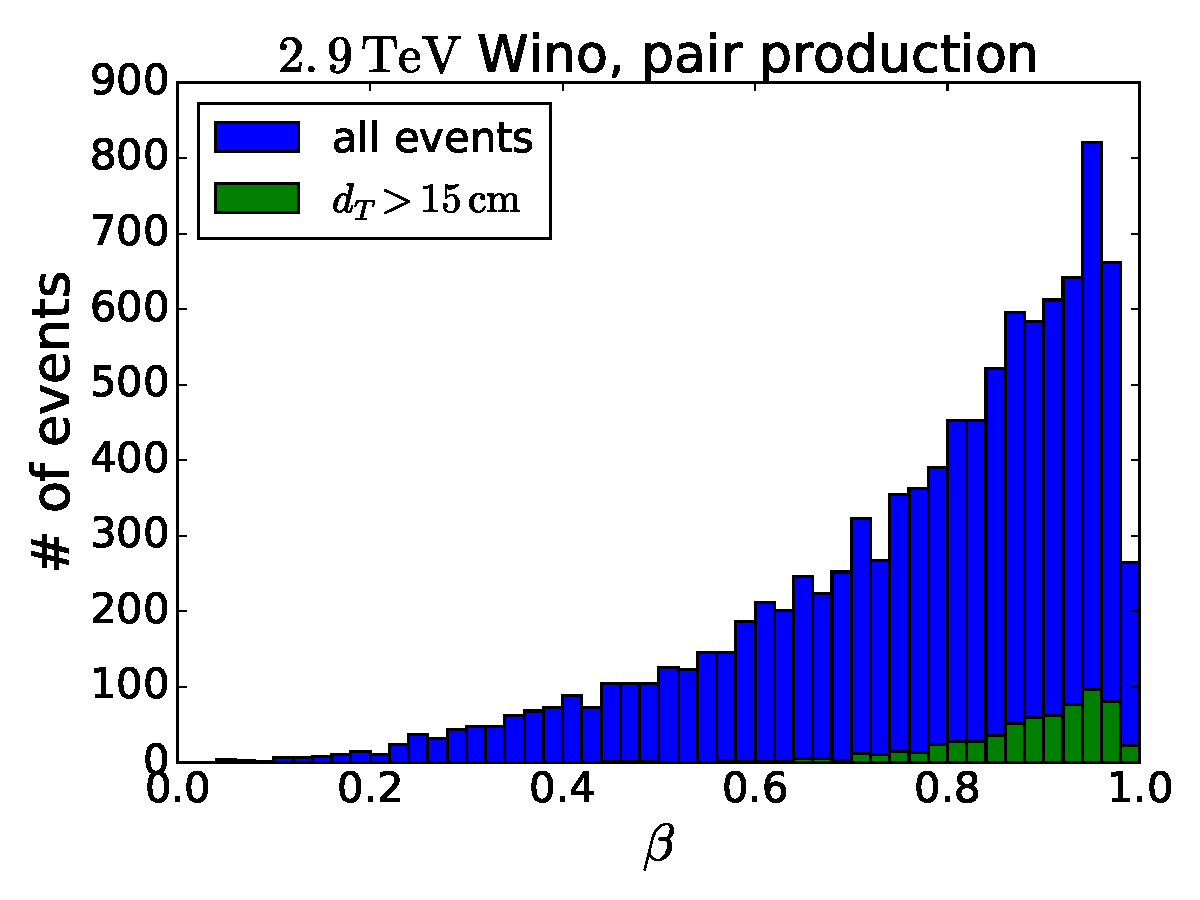
\includegraphics[width=0.5\hsize]{beta.pdf}
  \caption{
    Distribution of the Wino velocity $\beta$ for $2.9\,\mathrm{TeV}$ Wino.
    The pair prodction process at $\sqrt{s}=100\,\mathrm{TeV}$ and $\mathcal{L} = 30\,\mathrm{ab}^{-1}$ is assumed.
  }
  \label{fig:beta}
\end{figure}

In Fig.~\ref{fig:beta}, we show the distribution of the wino velocity $\beta$ for the same process.
The blue histogram shows the distribution of all winos, while the orange one shows that of winos with $d_T > 15\,\mathrm{cm}$, picked up according to the survival probability Eq.~\eqref{eq:survival_probability}.
As already seen in Fig.~\ref{fig:invariant_mass}, the center of mass energy of the two wino system distributes from a few to $\mathcal{O} (10) \,\mathrm{TeV}$, and many winos are highly boosted with $\beta \sim 1$.
Since a wino tends to fly for longer distance when it is more accelerated, some of boosted winos $\beta \gtrsim 0.6$ satisfy the requirement $d_T > 15\,\mathrm{cm}$.


\subsubsection*{Current constraints and future prospects}

The produced charged component of a WIMP is first detected by the trackers, which is equipped in the most inner part of detectors.
So far, the search is performed by both ATLAS \cite{Aaboud:2017mpt} and CMS \cite{Sirunyan:2018ldc} collborations.
Below, we will focus particularly on the ATLAS collaboration and discuss current constraints.

\begin{figure}[t]
  \centering
  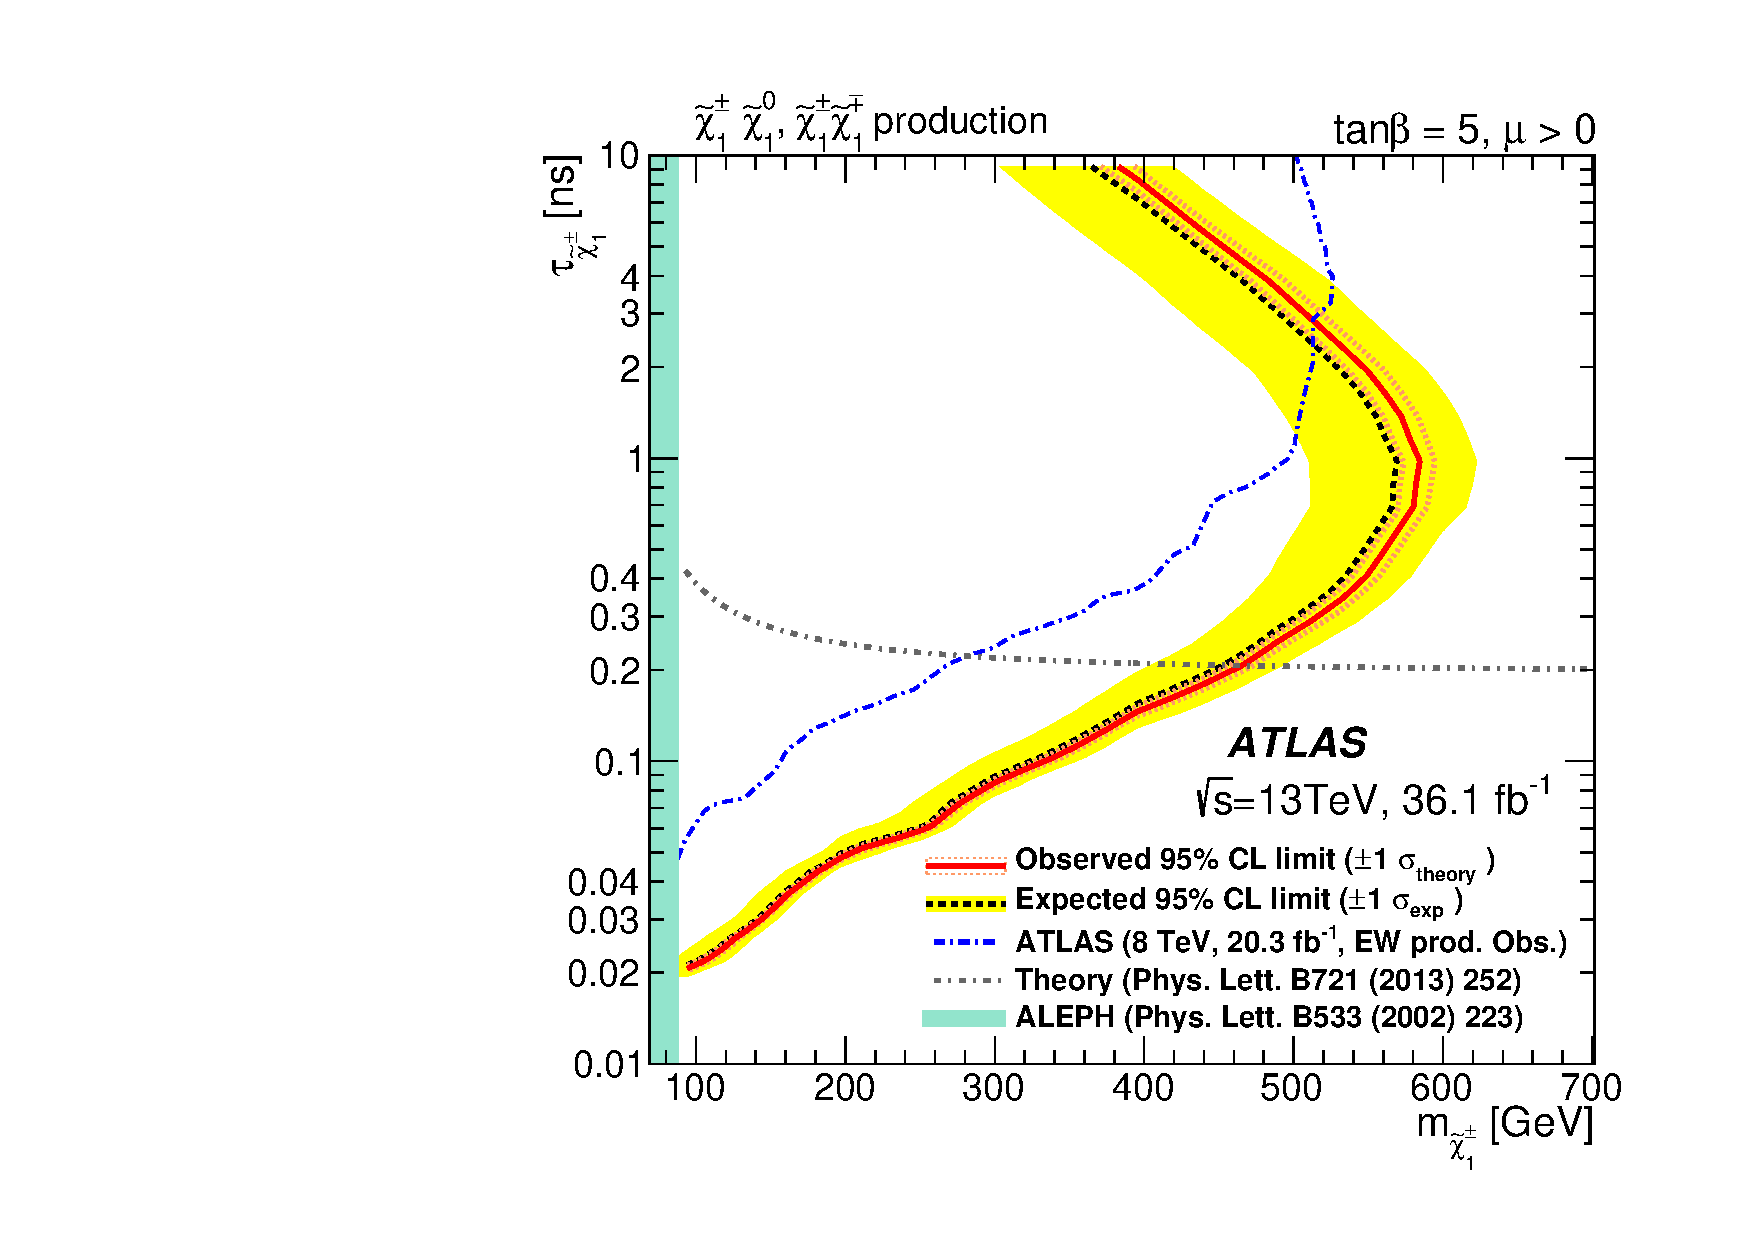
\includegraphics[width=0.5\hsize]{ATLAS_disappearing_track.pdf}
  \caption{Current status of the disappearing track search taken from \cite{Aaboud:2017mpt}.}
  \label{fig:ATLAS_disappearing_track}
\end{figure}

\begin{table}[t]
  \centering
  \begin{tabular}{c|ccc}
    WIMP & pure Higgsino & Wino & $5$-plet fermion \\ \hline
    Upper bound on $m_\chi$ & $120\, \mathrm{GeV}$ & $460\, \mathrm{GeV}$
    & $260\, \mathrm{GeV}$
  \end{tabular}
  \caption{
    Current upper bound for WIMP masses obtained from the disappearing track search shown in Fig.~\ref{fig:ATLAS_disappearing_track}.}
  \label{tab:disp_track_current}
\end{table}

In Fig.~\ref{fig:ATLAS_disappearing_track}, we show the result of the disappearing track search taken from \cite{Aaboud:2017mpt}.
The yellow band shows the current constraint on the WIMP mass and lifetime plane and the left part of the band is already excluded.
The sensitivity becomes weak when we consider $\tau \gtrsim 1\, \mathrm{ns}$ or $c \tau \gtrsim 30\, \mathrm{cm}$ due to the requirement of the SCT veto.
In the figure, the lifetime of Wino as a function of its mass is also shown by the black dot-dashed line.
It can be seen that the current contraint on Wino mass is $m_\chi \lesssim 460\,\mathrm{GeV}$.

Using the lifetime evaluated in the previous subsection, we summarize the current status for several WIMPs in Table \ref{tab:disp_track_current}, which exhibits upper limits of $\mathcal{O} (100)\,\mathrm{GeV}$.
However, note that the bound for the Higgsino listed in the table neglects the mixing between Higgsino and gauginos.
Actually, $\Delta m_{+}$ and thus $\tau$ are sensitive to the mixing, and an order estimation shows that the mixing lowers the lifetime to be $\tau \lesssim 0.01\,\mathrm{ns}$ and spoils the bound for Higgsino when $M_1$, $M_2 \lesssim 100\,\mathrm{TeV}$ (without any non-trivial cancellation in Eq.~\eqref{eq:Higgsino_delm_tree}).

The analysis of disappearing track search performed at future hadron colliders is performed in \cite{Han:2018wus, Saito:2019rtg}.
Since the detector setup for future colliders such as FCC-hh is undetermined yet, in \cite{Saito:2019rtg}, the authors assume several setups and compare the result.
In each setup, five layers of pixel detectors are installed and the fifth layer position (which we call $r_5$) ranges from $15\, \mathrm{cm}$ to $27\, \mathrm{cm}$.
\footnote{
  For simplicity of the discussion, we just assume that the detectors outside pixel detectors are far apart from the beam line so that all the WIMPs decay before reaching them.
  Then, we can estimate the discovery reach by counting the number of WIMP signals that reach the fifth layer of pixel detectors.
}
For the background reduction, hits to all of the five layers are required.
By varying the average number of $pp$ interactions per bunch crossing from $\Braket{\mu} = 200$ to $500$, the fake background rate is estimated to range from $10^{-7}$ to $10^{-5}$.

\begin{table}[t]
  \centering
  \begin{tabular}{c|cc}
    Detector setup & pure Higgsino & Wino \\ \hline
    $r_5 = 15\,\mathrm{cm}$ & $0.9$--$1.2\,\mathrm{TeV}$ & $> 4.0\,\mathrm{TeV}$ \\
    $r_5 = 27\,\mathrm{cm}$ & $<0.7\,\mathrm{TeV}$ & $2.9$--$4.0\,\mathrm{TeV}$
  \end{tabular}
  \caption{Prospects of $5\sigma$ discovery reach at FCC-hh with $\mathcal{L} = 30\,\mathrm{ab}^{-1}$ taken from \cite{Saito:2019rtg}.}
  \label{tab:disp_track_future}
\end{table}

In Table~\ref{tab:disp_track_future}, we summarize the obtained $5\sigma$ discovery reach for pure Higgsino and Wino for two detector setups with the integrated luminosity $\mathcal{L} = 30\,\mathrm{ab}^{-1}$.
The uncertainty of the reach corresponds the variation of $\Braket{\mu}=200$--$500$ and the uncertainty in soft QCD processes.
Recalling the discussion in Sec.~\rem{DM??}, Table~\ref{tab:disp_track_future} shows that FCC-hh can cover the whole region of the parameter space consistent with wino DM $m_\chi \lesssim 2.9\,\mathrm{TeV}$.
On the other hand, the well-motivated mass for Higgsino DM $m_\chi \sim 1.1\,\mathrm{TeV}$ can only be covered with the most optimistic assumption, \textit{i.e.}, the pure Higgsino with small $\Delta m_{+}$ searched for with $r_5 = 15\,\mathrm{cm}$.
Thus, it is an important task to consider another way of search for Higgisno, in particular a way that is unaffected by the mass difference $\Delta m_{+}$

\rem{Some comment on MDM?}


%%%%%%%%%%%%%%%%%%%%%%%%%%%%%%%%%%%%%%%%%%%%%%%%%%%%%%%%%%%%%%%%%%%%%%%%%%%%%%%
\subsection{Soft lepton search}
\label{sec:disappearing_track}
%%%%%%%%%%%%%%%%%%%%%%%%%%%%%%%%%%%%%%%%%%%%%%%%%%%%%%%%%%%%%%%%%%%%%%%%%%%%%%%

\rem{If possible}


%%%%%%%%%%%%%%%%%%%%%%%%%%%%%%%%%%%%%%%%%%%%%%%%%%%%%%%%%%%%%%%%%%%%%%%%%%%%%%%
\subsection{Mono-jet search}
\label{sec:disappearing_track}
%%%%%%%%%%%%%%%%%%%%%%%%%%%%%%%%%%%%%%%%%%%%%%%%%%%%%%%%%%%%%%%%%%%%%%%%%%%%%%%

\rem{For Higgsino search, cite} \cite{Baer:2014cua}.


% \bibliographystyle{elsarticle-num}
% \bibliography{../phd}

\end{document}


\clearpage

% Erase biblio in input file before turning on
\documentclass[12pt,twoside,book]{article}

\input{../settings}

\begin{document}


%%%%%%%%%%%%%%%%%%%%%%%%%%%%%%%%%%%%%%%%%%%%%%%%%%
\section[Indirect search of WIMPs using Drell-Yan process]{
  Indirect search of WIMPs\\
  using Drell-Yan process
}
\label{sec:dy}
\setcounter{equation}{0}
%%%%%%%%%%%%%%%%%%%%%%%%%%%%%%%%%%%%%%%%%%%%%%%%%%

\vskip 0.1in

\begin{figure}[b]
  \centering
  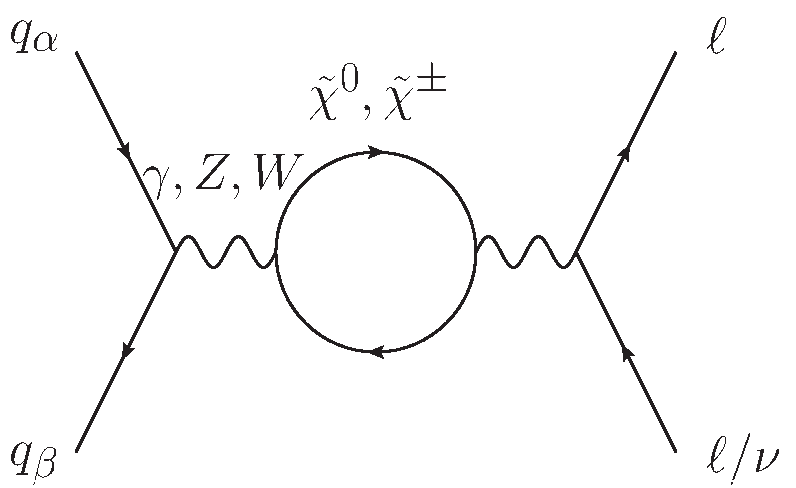
\includegraphics[width=0.5\hsize]{NC_CC_WIMP.pdf}
  \caption{WIMP effect on the Drell-Yan processes considered in this section.}
  \label{fig:NC_CC_WIMP}
\end{figure}

So far, we have discussed several ways to search for WIMPs using DM searches and collider experiments.
We have seen that, while WIMPs with relatively large $SU(2)_L$ charges such as Wino and the 5-plet fermion are promising for these searches, Higgsino is typically more challenging to probe.
Given this situation, another search strategy attracts a lot of attention~\cite{Chigusa:2018vxz, Abe:2019egv, Alves:2014cda, Harigaya:2015yaa, Gross:2016ioi, Farina:2016rws, Matsumoto:2017vfu, DiLuzio:2018jwd, Matsumoto:2018ioi} that probes WIMPs via the electroweak precision measurement at colliders.
It utilizes a pair production of charged leptons or that of a charged lepton and a neutrino, where WIMPs affect the pair production processes through the vacuum polarization of the electroweak gauge bosons as shown in Fig.~\ref{fig:NC_CC_WIMP}.
It is an indirect search method in the sense that it does not produce on-shell WIMPs as final states.

There are several virtues in this method such as the robustness against the change of the lifetime and the decay modes of WIMPs and the characteristic dip-like shape of the invariant mass distributions at the value close to twice the WIMP mass as we will see below.
We will see that the latter point helps us to distinguish the WIMP effects from backgrounds and systematic errors.
However, the obtained reach for Higgsino in most of the literature is still unsatisfactory since the use of the LHC or lepton colliders gives us only a small number of events at the position of the dip for a heavy Higgsino, which results in the reach much below the thermal Higgsino DM mass $m_\chi \sim 1\,\mathrm{TeV}$.

\begin{figure}[t]
  \centering
  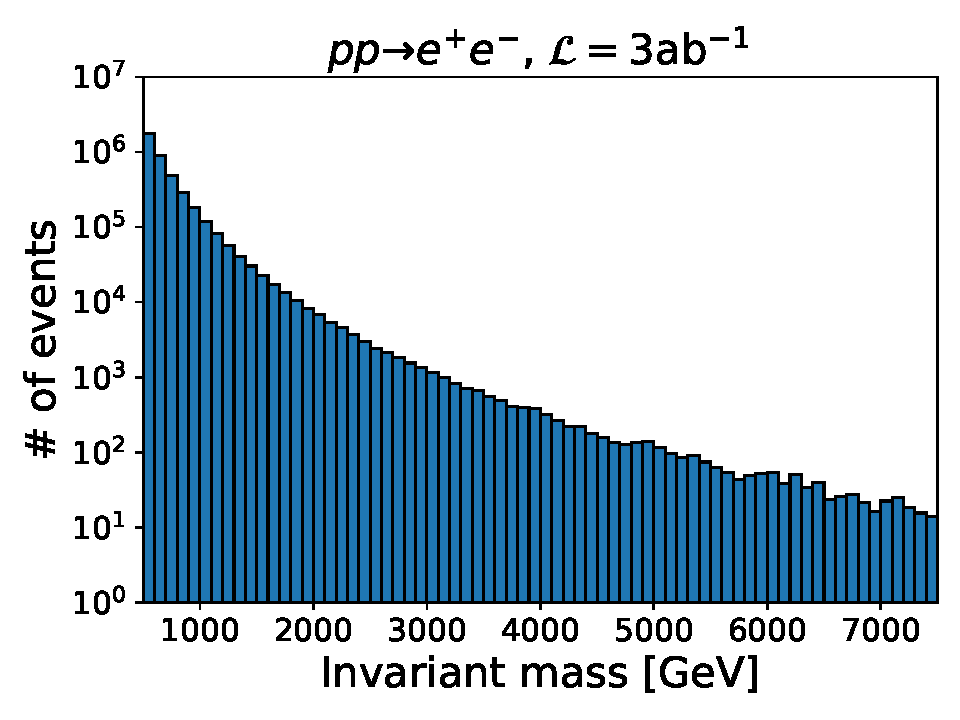
\includegraphics[width=0.5\hsize]{histMee.pdf}
  \caption{
    Invariant mass distribution of the pair-produced electrons at a $100\,\mathrm{TeV}$ collider with the integrated luminosity $\mathcal{L} = 3\,\mathrm{ab}^{-1}$.
  }
  \label{fig:histMee}
\end{figure}

Thus, in this section, we pursue this indirect search method further, considering a much higher CM energy using the future $100\,{\rm TeV}$ hadron colliders such as FCC-hh~\cite{Mangano:2016jyj, Contino:2016spe, Golling:2016gvc, Benedikt:2651300} and SppC~\cite{CEPC-SPPCStudyGroup:2015csa, CEPC-SPPCStudyGroup:2015esa}.
We concentrate on the Drell-Yan processes that have two charged leptons or mono-lepton plus a neutrino in the final state since they provide a very clean signal without any hadronic jets at least from the final state particles.
In Fig.~\ref{fig:histMee}, we show the invariant mass distribution of the pair produced electrons, for example, at a $100\,\mathrm{TeV}$ collider with the integrated luminosity $\mathcal{L} = 3\,\mathrm{ab}^{-1}$.
As we will discuss in Sec.~\ref{sec_event} in more detail, the NLO QCD effect is taken into account and \texttt{NNPDF2.3QED} with $\alpha_s (M_Z) = 0.118$~\cite{Ball:2013hta} is used as a canonical set of PDFs.
In the figure, events are divided into bins with equal width of $100\,\mathrm{GeV}$.
Thanks to the large CM energy, there are roughly $10^4$ events around the invariant mass of $2\,\mathrm{TeV}$ that can be used to probe the $\mathcal{O}(1)\,\%$ effect of the new physics, which will be turned out to be useful for the $1\,\mathrm{TeV}$ Higgsino search.

Below, we will show that the indirect search method provides \textit{a comparable or better experimental reach for Higgsino} compared to the direct production search of WIMPs at future colliders~\cite{Low:2014cba, Cirelli:2014dsa, Han:2018wus, Mahbubani:2017gjh}.
Besides, we demonstrate for the first time that the indirect search method can be applied not only to discover WIMPs but also \textit{to investigate their properties, such as charges, masses, and spins.}
To this end, it is important to consider both the charged current (CC) process with two-lepton final state and the neutral current (NC) process with mono-lepton final state to break some degeneracy among different WIMP charge assignments; the NC and CC processes depend on different combinations of the $SU(2)_L$ and $U(1)_Y$ charges of WIMP, and hence the inclusion of both processes allows us to extract these charges separately.

This section is based on our works \cite{Chigusa:2018vxz, Abe:2019egv}.


%%%%%%%%%%%%%%%%%%%%%%%%%%%%%%%%%%%%%%%%%%%%%%%%%%
\subsection{WIMP effect on the Drell-Yan processes}
\label{sec:WIMP}
%%%%%%%%%%%%%%%%%%%%%%%%%%%%%%%%%%%%%%%%%%%%%%%%%%

We investigate contributions of the WIMPs to the Drell-Yan processes through the vacuum polarization of the electroweak gauge bosons at the loop level.
Throughout this section, we assume that all the other beyond the SM particles are heavy enough so that they do not affect the following discussion.
After integrating out the WIMPs, the effective lagrangian relevant for our analysis is expressed as
\begin{align}
 \mathcal{L}_{\rm eff} = \mathcal{L}_{\rm SM} + C_2 g^2\, W_{\mu \nu}^a
 f\left(-\frac{D^2}{m^2}\right) W^{a\mu\nu} + C_1 g'^2\, B_{\mu\nu}
 f\left(-\frac{\partial^2}{m^2}\right) B^{\mu\nu},\label{eq_lag}
\end{align}
where $\mathcal{L}_{\rm SM}$ is the SM Lagrangian, $D$ is a covariant derivative, $m$ is the WIMP mass,\footnote
{
  Here we neglect a small mass splitting among the $SU(2)_L$ multiplet.
}
$g$ and $g'$ are the $SU(2)_L$ and $U(1)_Y$ gauge coupling constants, and $W_{\mu\nu}^a$ and $B_{\mu\nu}$ are the field strength associated with the $SU(2)_L$ and $U(1)_Y$ gauge group, respectively.
The function $f(x)$ is defined as \cite{Matsumoto:2017vfu}
\begin{align}
  f(x) = \begin{cases}
    \displaystyle{\frac{1}{16\pi^2} \int_0^1 dy\, (1-2y)^2 \ln (1-
    y(1-y)x - i0)} & {\rm (Scalar)},\\[5mm]
	  %%
    \displaystyle{\frac{1}{16\pi^2} \int_0^1 dy\, y(1-y) \ln (1 -
	  y(1-y)x - i0)} & {\rm (Fermion)},
  \end{cases}\label{eq_f}
\end{align}
where the first (second) line corresponds to a scalar (fermionic) WIMP, respectively.\footnote
{
  If a WIMP interacts only through the electroweak interaction, its decay width is of $\mathrm{O}(1)\%$ or less of its mass even if it is unstable.
  We assume that this is the case, and neglect the small effect on the function $f(x)$ due to the small decay width.
  Also, $f(x)$ corresponds to the finite part of the WIMP loop contribution after performing the renormalization in the $\overline{\mathrm{MS}}$ scheme.
}
The coefficients $C_1$ and $C_2$ for an $SU(2)_L$ $n$-plet WIMP with hypercharge $Y$ are given by
\begin{align}
 C_1 &= \frac{\kappa}{8} n Y^2,\label{eq_C1}\\
 %%
 C_2 &= \frac{\kappa}{8} I(n),\label{eq_C2}
\end{align}
where $\kappa = 1, 2, 8, 16$ for a real scalar, a complex scalar, a Weyl or Majorana fermion, and a Dirac fermion, respectively.
$I(n)$ is the Dynkin index for the $n$ dimensional representation of $SU(2)_L$ defined in Eq.~\eqref{eq:Dynkin}.
The coefficients are uniquely determined by the representation of the WIMPs.
For example, $(C_1, C_2) = (1, 1)$ for Higgsino, and $(C_1, C_2) = (0, 2)$ for Wino.
We emphasize that, contrary to the usual effective field theory, our prescription is equally applied when the typical scale of the gauge boson four-momentum $q$ is larger than the WIMP mass scale $m$ since we do not perform a derivative expansion of $f$ in
Eq.~\eqref{eq_lag}.
It is important because, as we see soon, the effect of the WIMPs is maximized when $q^2\sim m^2$, where the derivative expansion is not applicable.

\begin{table}[t]
  \centering
  \def\arraystretch{1.2}
  \begin{tabular}{c|cccccc}
    Fermion $f$ & $v_f^{(\gamma)}$ & $a_f^{(\gamma)}$ & $v_f^{(Z)}$ & $a_f^{(Z)}$ & $v_f^{(W)}$ & $a_f^{(W)}$ \\ \hline
    up-type quark & $\frac{2}{3}e$ & 0 & $(\frac{1}{4}-\frac{2}{3}s_W^2) g_Z$ & $-\frac{1}{4}g_Z$ & $\frac{1}{2\sqrt{2}}g$ & $-\frac{1}{2\sqrt{2}}g$ \\
    down-type quark & $-\frac{1}{3}e$ & 0 & $(-\frac{1}{4}+\frac{1}{3}s_W^2)g_Z$ & $\frac{1}{4}g_Z$ & $\frac{1}{2\sqrt{2}}g$ & $-\frac{1}{2\sqrt{2}}g$ \\
    lepton & $-e$ & 0 & $(-\frac{1}{4}+s_W^2)g_Z$ & $\frac{1}{4}g_Z$ & $\frac{1}{2\sqrt{2}}g$ & $-\frac{1}{2\sqrt{2}}g$ \\
  \end{tabular}
  \caption{Coefficients of the weak interaction defined as
    $\Gamma_f^{(V)} \equiv v_f^{(V)} + a_f^{(V)} \gamma_5$.  Here, $e = g
    s_W$ and $g_Z = g / c_W$, where $s_W \equiv \sin \theta_W$ and $c_W
    \equiv \cos \theta_W$ with $\theta_W$ being the weak mixing angle.}
  \label{table_weak}
\end{table}

At the leading order (LO), we are interested in $u(p)~\bar{u}(p') \to \ell^{-}(k)~\ell^{+}(k')$ and $d(p)~\bar{d}(p') \to \ell^{-}(k)~\ell^{+}(k')$ as the NC processes and $u(p)~\bar{d}(p') \to \nu(k)~\ell^{+}(k')$ and $d(p)~\bar{u}(p') \to \ell^{-}(k)~\bar{\nu}(k')$ as the CC processes.
Here, $u$ and $d$ collectively denote up-type and down-type quarks, respectively, and $p, p', k$, and $k'$ are initial and final state momenta.
In the SM, the amplitudes for both the NC and CC processes at the LO are expressed as
\begin{align}
 \mathcal{M}_{\rm SM} = \sum_{V} \frac{\left[ \bar{v}(p')
 \gamma^\mu \Gamma_q^{(V)} u(p) \right] \left[ \bar{u}(k) \gamma_\mu
 \Gamma_{\ell}^{(V)} v(k') \right]}{s' - m_V^2},\label{eq_m_sm}
\end{align}
where $\sqrt{s'}$ is the invariant mass of the final state leptons, which is denoted as $m_{\ell\ell}$ for the NC processes and $m_{\ell\nu}$ for the CC processes.
The relevant gauge bosons are $V = \gamma, Z$ for the NC processes and $V = W^\pm$ for the CC processes, with $m_V$ being the corresponding gauge boson mass.
In addition,
\begin{align}
  \Gamma_f^{(V)} \equiv v_f^{(V)} + a_f^{(V)} \gamma_5,
\end{align}
with $v_f^{(V)}$ and $a_f^{(V)}$ given in Tab.~\ref{table_weak}.
The WIMP contribution is given by
\begin{align}
 \mathcal{M}_{\rm WIMP} = \sum_{V,V'} C_{VV'} s' f\left(\frac{s'}{m^2}\right)
 \frac{\left[ \bar{v}(p') \gamma^\mu \Gamma_q^{(V)} u(p) \right]
 \left[ \bar{u}(k) \gamma_\mu \Gamma_\ell^{(V')} v(k') \right]}
 {(s'-m_V^2)(s'-m_{V'}^2)},\label{eq_m_WIMP}
\end{align}
where $C_{\gamma \gamma} = 4(C_1 g'^2 c_W^2 + C_2 g^2 s_W^2)$, $C_{\gamma Z} = C_{Z \gamma} = 4(C_2 g^2 - C_1 g'^2) s_W c_W$, $C_{Z Z} = 4(C_1 g'^2 s_W^2 + C_2 g^2 c_W^2)$, and $C_{WW} = 4 C_2 g^2$.
Again $V, V' = \gamma, Z$ for the NC processes and $V, V' = W^\pm$ for the CC processes.

We use $d\Pi_{\mathrm{LIPS}}$ for a Lorentz invariant phase space factor for the two-particle final state.
Then, using Eqs.~\eqref{eq_m_sm} and~\eqref{eq_m_WIMP}, we define
\begin{align}
 \frac{d \sigma_{\rm SM}}{d\sqrt{s'}} &= \sum_{\alpha, \beta}
 \frac{dL_{\alpha \beta}}{d\sqrt{s'}} \int d\Pi_{\mathrm{LIPS}}\, \left| \mathcal{M}_{\rm SM} \left( q_\alpha q_\beta \to \ell\ell / \ell\nu \right) \right|^2,\label{eq_sig_sm}\\
 %%
 \frac{d \sigma_{\rm WIMP}}{d\sqrt{s'}} &= \sum_{\alpha, \beta}
 \frac{dL_{\alpha \beta}}{d\sqrt{s'}} \int d\Pi_{\mathrm{LIPS}}\, 2 \Re \left[ \mathcal{M}_{\rm SM}
 \mathcal{M}_{\rm WIMP}^{*} \left( q_\alpha q_\beta \to \ell\ell / \ell\nu
 \right) \right],\label{eq_sig_WIMP}
\end{align}
where we take the average and summation over spins.\footnote{
  In Eq.~\eqref{eq_sig_WIMP}, we only take into account the contribution from WIMPs at the leading order of $g^{'2}$ and $g^2$, which corresponds to the real part of the loop function Eq.~\eqref{eq_f}.
  The contribution from the imaginary part may be enhanced by a sizable numerical factor, but we neglect it simply because it is a higher order term of the gauge coupling expansion.
}
Here, $dL_{\alpha \beta} / d\sqrt{s'}$ is the so-called luminosity function for a fixed
$\sqrt{s'}$:
\begin{align}
 \frac{d L_{\alpha \beta}}{d\sqrt{s'}} \equiv \frac{1}{s} \int_0^1 dx_1
 dx_2~f_\alpha(x_1) f_\beta(x_2) \delta\left(\frac{s'}{s} - x_1 x_2\right),
\end{align}
where $\alpha$ and $\beta$ denote species of initial partons, $\sqrt{s} = 100\,{\rm TeV}$, and $f_a(x)$ is the PDF used in Sec.~\ref{sec:wimp_production}.
Eq.\,\eqref{eq_sig_sm} represents the SM cross section, while Eq.\,\eqref{eq_sig_WIMP} the WIMP contribution to the cross section.
For the statistical treatment in the next section, we introduce a parameter $\mu$ that parametrizes the strength of the WIMP effect and express the cross section with $\mu$ as
\begin{align}
 \frac{d\tilde{\sigma}}{d\sqrt{s'}} =
 \frac{d\sigma_{\rm SM}}{d\sqrt{s'}}
 + \mu \frac{d\sigma_{\rm WIMP}}{d\sqrt{s'}}.
 \label{eq_diffcrosssection}
\end{align}
Obviously, $\mu=0$ corresponds to the pure SM, while $\mu=1$ corresponds to the SM$+$WIMP model.
Hereafter, we use
\begin{align}
 \delta_\sigma ( \sqrt{s'} ) \equiv \frac{d\sigma_{\rm
 WIMP} / d\sqrt{s'}}{d\sigma_{\rm SM} /
 d\sqrt{s'}},\label{eq_dsigma}
\end{align}
to denote the correction from the WIMP.
Note that this ratio remains unchanged even if we take into account the next-to-leading order (NLO) QCD effect because the EWIMPs affect the cross sections only through the vacuum polarization.\footnote
{
  When the NLO QCD effect is included, one of the initial partons can be gluon with the real emission of one jet in the final state.
  However, we can easily see that $\delta_\sigma^{ug}$ = $\delta_\sigma^{uu}$ and so on.
}

\begin{figure}[t]
  \centering
  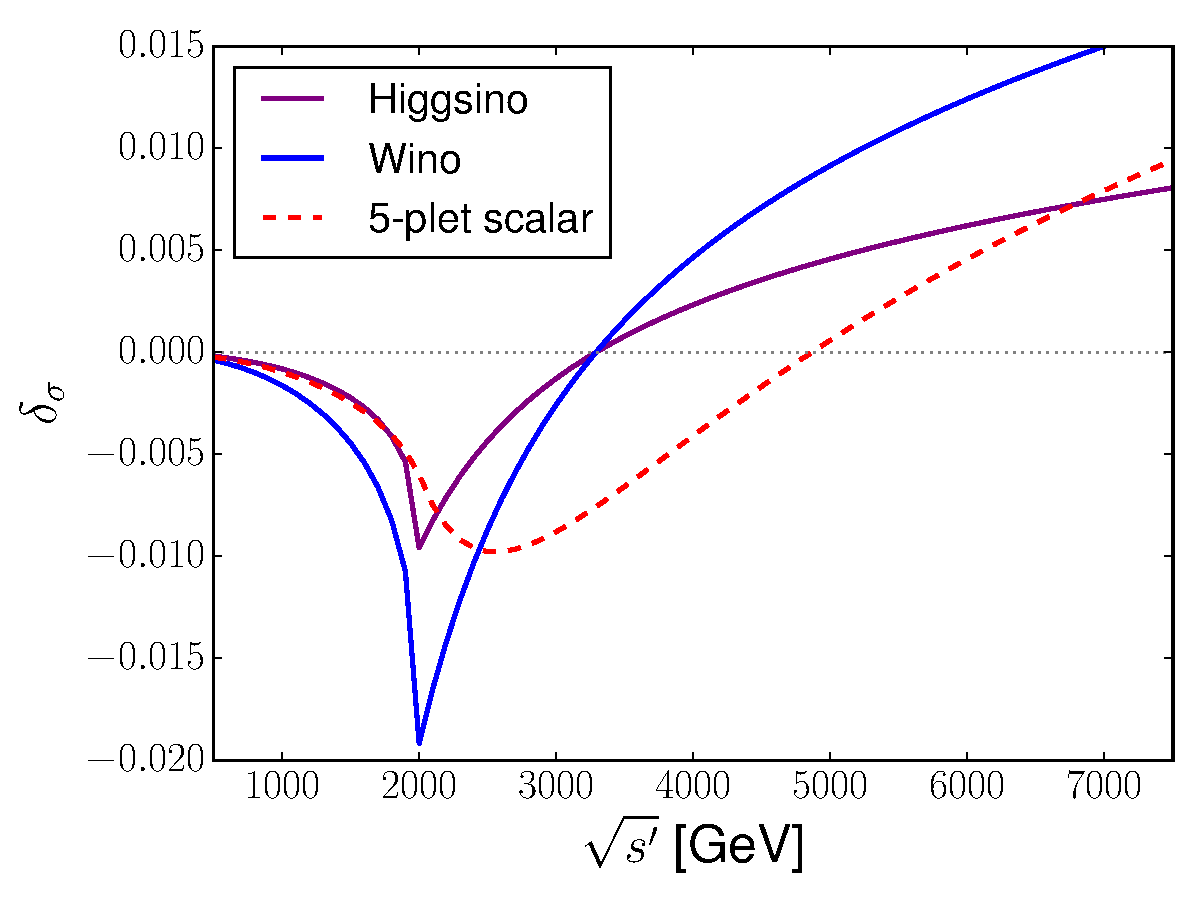
\includegraphics[width=0.5\hsize]{sqsp_vs_del.pdf}
  \caption{
    $\delta_\sigma$ for the CC processes as a function of $\sqrt{s'} = m_{\ell\nu}$.
    The purple, blue, and red lines correspond to Higgsino, Wino, and 5-plet real scalar, respectively.
  }
  \label{fig_sqsp_vs_del}
\end{figure}

In Fig.~\ref{fig_sqsp_vs_del}, we plot $\delta_\sigma$ for the CC processes as a function of $\sqrt{s'}$.
The purple, blue, and red lines correspond to Higgsino, Wino, and 5-plet scalar, respectively.
There is a dip around $\sqrt{s'} = 2m$ for all the cases of the WIMPs which originates from the loop function $f$ in Eq.~\eqref{eq_f}.
The WIMP contributions to the NC processes show a similar dip structure that again comes from $f$.
This dip is crucial not only for the discovery of the WIMP signal (see Sec.~\ref{sec_detection}) but also for the determination of the properties of the WIMPs (see Sec.~\ref{sec_property}).
In particular, the WIMP mass can be extracted from the dip position, while the WIMP charges ($n$ and $Y$) can be determined from the depth of the dip.
The negative sign of the WIMP contributions can be understood from the consideration using the optical theorem and the analytic structure of the loop function.
See Appendix \ref{sec:reim} for the detailed discussion.

\begin{figure}[t]
  \centering
  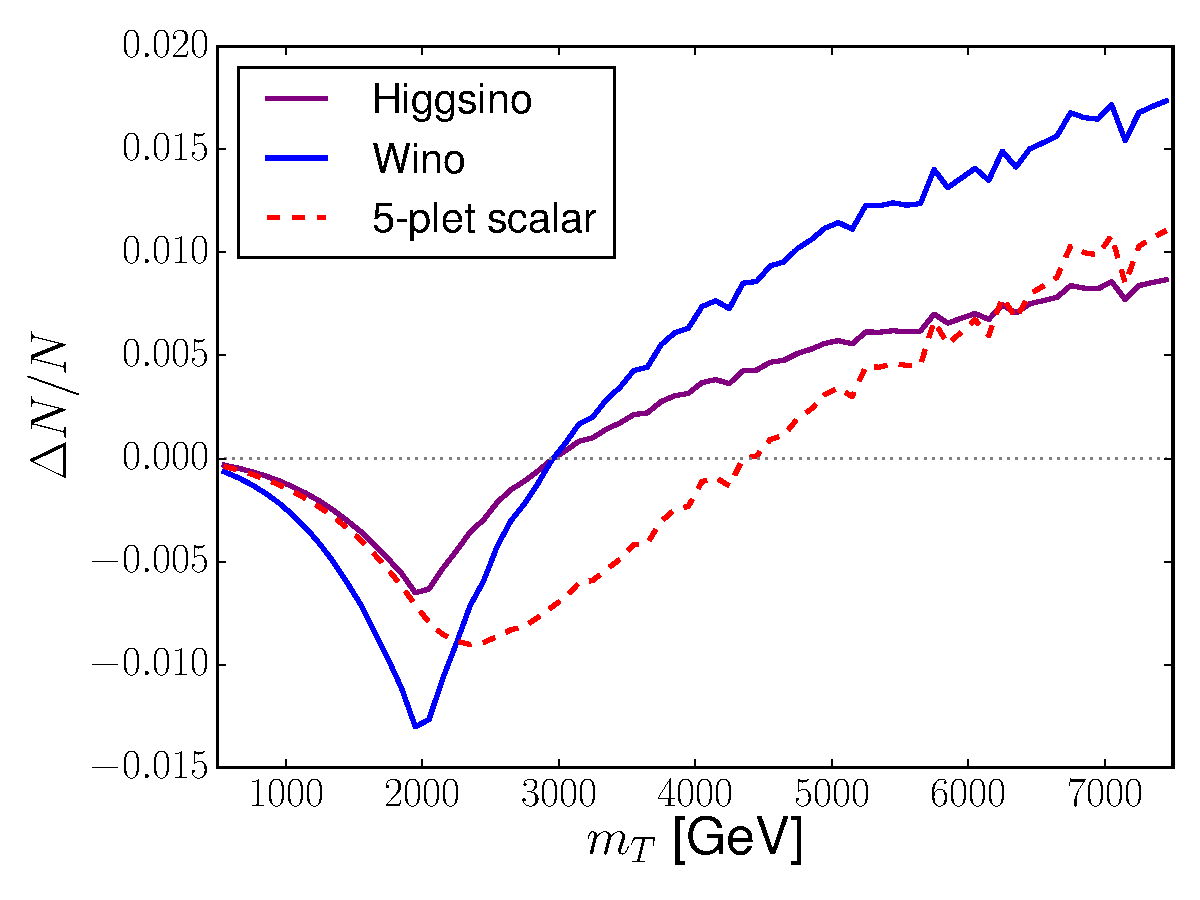
\includegraphics[width=0.5\hsize]{mT_vs_del.pdf}
  \caption{
    The WIMP effect on the ratio of the number of events $\Delta N / N$ as a function of $m_T$.
    The line colors are the same as Fig.~\ref{fig_sqsp_vs_del}.
  }
  \label{fig_mT_vs_dN}
\end{figure}

For the NC processes, the momenta of two final state charged leptons are measurable and we can use the invariant mass distribution of the number of events for the study of the WIMPs.
For the CC processes, on the contrary, we cannot measure the momentum of the neutrino in real experiments, and hence we instead use the missing transverse momentum $\Slash{p}_T$.
We use the transverse mass defined as
\begin{align}
  m_T^2 \equiv 2 p_{T, \ell}\,\Slash{p}_T \left( 1-\cos \phi \right),
\end{align}
where $p_{T, \ell}$ denotes the transverse momentum of the charged lepton and $\phi$ is the difference between the azimuth angles of $p_{T,\ell}$ and $\Slash{p}_T$.
The important property of $m_T$ is that the distribution of $m_T$ peaks at $m_T = m_{\ell\nu}$ (see Appendix~\ref{sec:mT} for more detailed description of the quantity $m_T$).
Because of this property, the characteristic shape of $\delta_\sigma$ remains in the $m_T$ distribution in the CC events.
To see this, we plot in Fig.~\ref{fig_mT_vs_dN} the WIMP effect on the number of events as a function of $m_T$.
Here, the vertical axis is the ratio of the WIMP correction to the number of events $\Delta N$ to the number of events in the SM $N$ for each bin with the bin width of $100\, {\rm GeV}$.\footnote
{
  Just for an illustrative purpose, we generate events corresponding to the integrated luminosity $\mathcal{L} = 1\,\mathrm{ab}^{-1}$ for this figure, which is not the same luminosity as we use in the next section (see Sec.~\ref{sec_event} for details of the event generation).
}
We find that the dip structure remains in the $m_T$ distribution, though the depth of the dip is smaller compared to the $m_{\ell\nu}$ distribution.


%%%%%%%%%%%%%%%%%%%%%%%%%%%%%%%%%%%%%%%%%%%%%%%%%%
\subsection{Analysis}
\label{sec:analysis}
%%%%%%%%%%%%%%%%%%%%%%%%%%%%%%%%%%%%%%%%%%%%%%%%%%


%%%%%%%%%%%%%%%%%%%%%%%%%%%%%%%%%%%%%%%%%%%%%%%%%%
\subsubsection{Event generation}
\label{sec_event}
%%%%%%%%%%%%%%%%%%%%%%%%%%%%%%%%%%%%%%%%%%%%%%%%%%

Now we discuss how well we can extract information about WIMPs from the invariant mass and transverse mass distributions for the processes of our concern at future $100\,\mathrm{TeV}$ $pp$ collider experiments.
We take into account the effects of the next-to-leading order QCD corrections in the events as well as detector effects through Monte-Carlo simulations.

In our analysis, we first generate the SM event sets for the NC processes $pp\to e^{-}e^{+} / \mu^{-}\mu^{+}$ and the CC processes $pp\to e^{\pm}\nu_e / \mu^{\pm}\nu_\mu$.
We use \texttt{MadGraph5\_aMC@NLO} (\texttt{v2.6.3.2})~\cite{Alwall:2011uj, Alwall:2014hca} for the event generation with the successive use of \texttt{Pythia8}~\cite{Sjostrand:2014zea} for the parton shower and the hadronization and \texttt{Delphes} (\texttt{v3.4.1})~\cite{deFavereau:2013fsa} with the card {\tt FCChh.tcl} for the detector simulation.
We use \texttt{NNPDF2.3QED} with $\alpha_s (M_Z) = 0.118$~\cite{Ball:2013hta} as a canonical set of PDFs.
For the renormalization and factorization scales, we use the default values of \texttt{MadGraph5\_aMC@NLO}, i.e., the central $m_T^2$ scale after $k_T$-clustering of the event (which we denote by $Q$).
We take into account the NLO QCD effect by the \verb|[QCD]| option of \verb|MadGraph5_aMC@NLO| which enhances the cross section roughly by a factor of $2$ compared to the LO calculation.\footnote
{
  This large enhancement implies that the next-to-next-to-leading order QCD effect may also have a non-negligible effect on the cross section, and its calculation remains as a future task.
  However, due to its smooth dependence on $\sqrt{s'}$, it may not much affect the detection reach of the EWIMPs.
  See Sec.~\ref{sec_statistical} for the details.
}
The events are binned by the characteristic mass $m_{\mathrm{char}}$ for each process: we use the lepton invariant mass $m_{\mathrm{char}} = m_{\ell\ell}$ for the NC processes, and the transverse mass $m_{\mathrm{char}} = m_T$ for the CC processes, respectively.
In both cases, we generated events with the characteristic mass within the range of $500\,\mathrm{GeV} < m_\mathrm{char} < 7.5\,\mathrm{TeV}$ and divide them into $70$ bins with an equal width of $100\,\mathrm{GeV}$.

As for the event selection by a trigger, we may have to impose some cut on the lepton transverse momentum $p_T$.
As we will see, we concentrate on events with high $p_T$ charged lepton(s) with which we expect the event may be triggered.
For the NC processes, we use events with at least two high $p_T$ leptons.  For our analysis, we use events with $m_{\ell\ell}>500\ {\rm GeV}$; we assume that such events are triggered by using two energetic charged leptons so that we do not impose any other kinematical requirement at the parton level.\footnote{
  Note that the simplified geometry of detector layout is included in the \texttt{Delphes} card and, for example, muons with large absolute pseudorapidity $|\eta| > 6$ are automatically neglected at the detector simulation.
}
On the contrary, the CC events are characterized only by a lepton and a missing transverse momentum.
For such events, we require that the $p_T$ of the charged lepton should be larger than $500\,\mathrm{GeV}$.
\footnote{
  In the ATLAS analysis of the mono-lepton signal during the 2015 (2016) data taking period~\cite{Aaboud:2017efa}, they use the event selection condition $p_T > 24\, (60)\,\mathrm{GeV}$ for leptons that satisfy the \textit{medium} identification criteria.
  In the CMS analysis during the period on 2016~\cite{Sirunyan:2018mpc}, they use the condition $p_T > 130 (53)\, \mathrm{GeV}$ for an electron (a muon).
}
For the CC events, the cut reduces the number of events in particular for the bins with the low transverse mass $m_T \sim 500\, \mathrm{GeV}$, and thus affects the sensitivity of the CC processes to relatively light WIMPs.
We will come back to this point later.


The WIMP effect is incorporated by rescaling the SM event by $\delta_\sigma$ defined in Eq.~\eqref{eq_dsigma}.
With the parameter $\mu$ defined in Eq.~\eqref{eq_diffcrosssection}, the number of events corresponding to the SM+WIMP hypothesis in $i$-th bin, characterized by $m_{i, \mathrm{min}} < m_{\mathrm{char}} < m_{i, \mathrm{max}}$, is
\begin{align}
  x_{f,i} (\mu) = \sum_{\substack{\text{events that satisfy}\\m_{i, \mathrm{min}} < m_{\mathrm{char}} < m_{i, \mathrm{max}}}}
  \left[
    1 + \mu \delta_\sigma (\sqrt{s'})
  \right],
  \label{eq_n_tot}
\end{align}
where the sum runs over all the events of the final state $f$ whose characteristic mass $m_{\mathrm{char}}$ (after taking into account the detector effects) falls into the bin.
Note that the true value of $\sqrt{s'}$ should be used for each event for the computation of $\delta_\sigma$: we extract it from the hard process information.\footnote
{
	The $p_T$ cut for the CC process does not affect this estimation since the WIMP does not modify the angular distribution of the final lepton and neutrino for the CC process.
}


%%%%%%%%%%%%%%%%%%%%%%%%%%%%%%%%%%%%%%%%%%%%%%%%%%
\subsubsection{Statistical treatment}
\label{sec_statistical}
%%%%%%%%%%%%%%%%%%%%%%%%%%%%%%%%%%%%%%%%%%%%%%%%%%

We now explain the statistical method we will adopt in our analysis.
Throughout this section, we rely on the so-called profile likelihood method, which is described in detail in Appendix \ref{sec:profile}.
We collectively denote our theoretical model as $\bm{x}_f(\mu) = \{ x_{f,i} (\mu) \}$, where $x_{f,i}(\mu)$ is given by Eq.~\eqref{eq_n_tot}.
We denote the experimental data set as $\check{\bm{x}}_f$ that in principle is completely unrelated to our theoretical model $\bm{x}_f(\mu)$.
Since we do not have an actual experimental data set for $100~\,\mathrm{TeV}$ colliders for now, however, we take $\check{\bm{x}}_f = \bm{x}_f(\mu = 1)$ (for some fixed values of the WIMP mass and charges) throughout our analysis, assuming that the WIMP does exist.  In particular, this choice tests the SM-only hypothesis if we take our theoretical model as $\bm{x}_f(\mu=0)$.

If the expectation values of $x_{f,i} (\mu)$ are precisely known, the sensitivity to WIMPs can be studied only with statistical errors.
In reality, however, the computation of $x_{f,i} (\mu)$ suffers from various sources of uncertainties, which results in systematic errors in our theoretical model.
The sources include errors in the integrated luminosity, the beam energy, choices of the renormalization and the factorization scales, choices of PDF, the pile-up effect, higher order corrections to the cross section, and so on.
In order to deal with these uncertainties, we introduce sets of free parameters $\bm{\theta}_f = \{ \theta_{f,\alpha} \}$ (i.e. nuisance parameters) which absorb (smooth) uncertainties of the number of events, and modify our theoretical model as
\begin{align}
  \tilde{x}_{f,i} (\bm{\theta}_f, \mu) \equiv x_{f,i} (\mu)
  f_{\mathrm{sys}, i}(\bm{\theta}_f),\label{eq_xtilde}
\end{align}
where $f_{\mathrm{sys}, i}(\bm{\theta}_f)$ is a function that satisfies $f_{\mathrm{sys}, i}(\bm{0}) =1$.
We expect that, if the function $f_{\mathrm{sys}, i}$ is properly chosen, the true distribution of the number of events in the SM is given by $\tilde{\bm{x}}_f (\bm{\theta}_f,0) = \{ \tilde{x}_{f,i} (0) f_{\mathrm{sys}, i}(\bm{\theta}_f)\}$ for some value of $\bm{\theta}_f$.
In our analysis, we adopt the five parameters fitting function given by~\cite{Aaltonen:2008dn}
\begin{align}
  f_{\mathrm{sys}, i} (\bm{\theta}_f) =
  e^{\theta_{f,1}} (1 - p_i)^{\theta_{f,2}}
  p_i^{(\theta_{f,3} + \theta_{f,4} \ln p_i + \theta_{f,5} \ln^2 p_i)},
  \label{eq_f_theta}
\end{align}
where $p_i = 2m_{i} / \sqrt{s}$ with $m_i$ being the central value of the lepton invariant mass (transverse mass) of the $i$-th bin for the NC (CC) processes.
As we will see, the major effects of systematic errors can be absorbed into $\bm{\theta}_f$ with this fitting function.

To test the SM-only hypothesis, we define the following test statistic~\cite{Cowan:2010js}:
\begin{align}
  q_0 \equiv -2 \sum_{f=\ell \ell, \ell \nu} \ln \frac
  {L(\check{\bm{x}}_f ; \doublehat{\bm{\theta}}_f, \mu=0)}
  {L(\check{\bm{x}}_f ; \hat{\bm{\theta}}_f, \hat{\mu})}.
  \label{eq_q0}
\end{align}
Here, $\doublehat{\bm{\theta}}_f$ and $\{ \hat{\bm{\theta}}_f, \hat{\mu} \}$ are determined so that $\prod_f L(\check{\bm{x}}_f ; \bm{\theta}_f, \mu=0)$ and $\prod_f L(\check{\bm{x}}_f ; \bm{\theta}_f, \mu)$ are maximized, respectively.
The likelihood function is defined as
\begin{align}
  L(\check{\bm{x}}_f ; \bm{\theta}_f, \mu) &\equiv
  L_{\bm{\theta}_f} (\check{\bm{x}}_f ; \mu) L'(\bm{\theta}_f ; \bm{\sigma}_f),
  \label{eq_L}
\end{align}
where
\begin{align}
  L_{\bm{\theta}_f} (\check{\bm{x}}_f ; \mu) &\equiv
  \prod_{i} \exp \left[
  -\frac{(\check{x}_{f,i} - \tilde{x}_{f,i} (\bm{\theta}_f, \mu))^2}
  {2 \tilde{x}_{f,i} (\bm{\theta}_f, \mu)}
  \right],
  \label{eq_Ltheta}\\
  %%
  L'(\bm{\theta}_f ; \bm{\sigma}_f) &\equiv
  \prod_{\alpha} \exp \left[
  - \frac{\theta_{f,\alpha}^2}{2\sigma_{f,\alpha}^2}
  \right].
  \label{eq_Lprime}
\end{align}
The product in Eq.\,\eqref{eq_Ltheta} runs over all the bins, while the product in Eq.\,\eqref{eq_Lprime} runs over all the free parameters we introduced.
For each $\theta_{f, \alpha}$, we define the ``standard deviation'' $\sigma_{f, \alpha}$, which parametrizes the possible size of $\theta_{f, \alpha}$ within the SM with the
systematic errors.\footnote
{
  Here we assume the Gaussian form for the nuisance parameter distribution.  The dependence of the results on the choice of the distribution will be discussed later in Sec.~\ref{sec_detection}.
}
If the systematic errors are negligible compared with the statistical error, we can take $\bm{\sigma}_f \to \bm{0}$, while the analysis with $\bm{\sigma}_f \to \infty$ assumes no knowledge of systematic errors and gives a conservative result.
We identify $\sqrt{q_0} = 5$ $(1.96)$ as the detection reach at the $5\sigma$ ($95\,\%$ C.L.) level, since $q_0$ asymptotically obeys a chi-square distribution with the degree of freedom one.

In order to determine $\bm{\sigma}_f$, we consider the following sources of the systematic errors:
\begin{itemize}
  \item Luminosity ($\pm 5\,\%$ uncertainty is assumed),
  \item Renormalization scale ($2Q$ and $Q/2$, instead of $Q$),
  \item Factorization scale ($2Q$ and $Q/2$, instead of $Q$),
  \item PDF choice (We use $101$ variants of \texttt{NNPDF2.3QED} with $\alpha_s (M_Z) = 0.118$~\cite{Ball:2013hta} provided by \texttt{LHAPDF6}~\cite{Buckley:2014ana} with IDs ranging from $244600$ to $244700$).
\end{itemize}
The values of $\bm{\sigma}_f$ are determined as follows.
Let $\bm{y}_f$ be the set of number of events in the SM for the final state $f$ with the canonical choices of the parameters, and $\bm{y}'_f$ be that with one of the sources of the systematic errors being varied.
We minimize the chi-square function defined as
\begin{align}
  \chi^2_f &\equiv \sum_i \frac
  {\left( y_{f,i}' - \tilde{y}_{f,i} (\bm{\theta}_f) \right)^2}
  {\tilde{y}_{f,i} (\bm{\theta}_f)},
\end{align}
where
\begin{align}
  \tilde{y}_{f,i} (\bm{\theta}_f) &\equiv
  y_{f,i} f_{\mathrm{sys},i} (\bm{\theta}_f),
\end{align}
for each final state $f$, and determine the best-fit values of $\bm{\theta}_f$ for each set of $\bm{y}'_f$.
We repeat this process for different sets of $\bm{y}'_f$, and $\bm{\sigma}_f$ are determined from the distributions of the best-fit values of $\bm{\theta}_f$.
For example, let us denote the best-fit values for the fit associated with the luminosity errors $\pm 5\%$ as $\bm{\theta}_f^{\pm}$.
We estimate $\bm{\sigma}_f$ associated with these errors, denoted here as $\bm{\sigma}_f^{\mathrm{lumi.}}$, as
\begin{align}
  \sigma_{f,\alpha}^{\mathrm{lumi.}} = \sqrt{\frac{(\theta_{f,\alpha}^{+})^2 + (\theta_{f,\alpha}^{-})^2}{N}},
\end{align}
where $N$ denotes the number of fitting procedures we have performed: $N=2$ for this case.
We estimate $\bm{\sigma}_f$ associated with the other sources of the errors, denoted as $\bm{\sigma}_f^{\mathrm{ren.}}$, $\bm{\sigma}_f^{\mathrm{fac.}}$, and $\bm{\sigma}_f^{\mathrm{PDF}}$, in a similar manner.
Finally, the total values of $\bm{\sigma}_f$ are obtained by combining all the sources together as\footnote
{
  There may be some correlations between the distribution of nuisance parameters $\bm{\theta}_{f}$.
  After the $100\,\mathrm{TeV}$ collider experiments will start and the sufficient amount of data will be accumulated, we should extract the information of correlations and use it to perform the analysis.
  However, because the real data does not exist yet, we rely on a simplified analysis in this section, treating each of them as obeying to an independent Gaussian distribution.
}
\begin{align}
  \sigma_{f,\alpha} = \sqrt{(\sigma_{f,\alpha}^{\mathrm{lumi.}})^2
  + (\sigma_{f,\alpha}^{\mathrm{ren.}})^2
  + (\sigma_{f,\alpha}^{\mathrm{fac.}})^2
  + (\sigma_{f,\alpha}^{\mathrm{PDF}})^2}.
  \label{eq_comb_sig}
\end{align}

\begin{table}[t]
  \centering
  \begin{tabular}{c|ccccc}
    Sources of systematic errors & $\sigma_{ee,1}$ & $\sigma_{ee,2}$ & $\sigma_{ee,3}$ & $\sigma_{ee,4}$ & $\sigma_{ee,5}$ \\ \hline
    Luminosity: $\pm 5\,\%$ ($\bm{\sigma}_{ee}^{\mathrm{lumi.}}$) & $0.05$ & $0$ & $0$ & $0$ & $0$ \\
    Renormalization scale: $2Q, Q/2$ ($\bm{\sigma}_{ee}^{\mathrm{ren.}}$) & $0.4$ & $0.6$ & $0.3$ & $0.05$ & $0.004$ \\
    Factorization scale: $2Q, Q/2$ ($\bm{\sigma}_{ee}^{\mathrm{fac.}}$) & $0.3$ & $0.5$ & $0.2$ & $0.06$ & $0.004$ \\
    PDF choice ($\bm{\sigma}_{ee}^{\mathrm{PDF}}$) & $0.4$ & $0.7$ & $0.3$ & $0.06$ & $0.004$
  \end{tabular}
  \caption{
    Values of $\bm{\sigma}_{ee}$ for each source of systematic errors.
    The result is the same for the $\mu\mu$ final state.
  }
  \label{tab_sys_ee}
\end{table}

\begin{table}[t]
  \centering
  \begin{tabular}{c|ccccc}
    Sources of systematic errors & $\sigma_{e \nu_e,1}$ & $\sigma_{e \nu_e,2}$ & $\sigma_{e \nu_e,3}$ & $\sigma_{e \nu_e,4}$ & $\sigma_{e \nu_e,5}$ \\ \hline
    Luminosity: $\pm 5\,\%$ ($\bm{\sigma}_{e \nu_e}^{\mathrm{lumi.}}$) & $0.05$ & $0$ & $0$ & $0$ & $0$ \\
    Renormalization scale: $2Q, Q/2$ ($\bm{\sigma}_{e \nu_e}^{\mathrm{ren.}}$) & $0.3$ & $0.4$ & $0.2$ & $0.04$ & $0.003$ \\
    Factorization scale: $2Q, Q/2$ ($\bm{\sigma}_{e \nu_e}^{\mathrm{fac.}}$) & $1.0$ & $1.6$ & $0.6$ & $0.1$ & $0.01$ \\
    PDF choice ($\bm{\sigma}_{e \nu_e}^{\mathrm{PDF}}$) & $0.6$ & $0.9$ & $0.4$ & $0.08$ & $0.006$
  \end{tabular}
  \caption{
    Best fit values of fit parameters for several sources of systematic errors for the $e\nu_e$ final state.
    The result is the same for the $\mu\nu_\mu$ final state.
  }
  \label{tab_sys_ev}
\end{table}

\begin{table}[t]
  \centering
  \begin{tabular}{c|ccccc}
    Final state $f$ & $\sigma_{f,1}$ & $\sigma_{f,2}$ & $\sigma_{f,3}$ & $\sigma_{f,4}$ & $\sigma_{f,5}$ \\ \hline
    $ee$ & $0.7$ & $1.0$ & $0.4$ & $0.09$ & $0.008$ \\
    $\mu\mu$ & $0.7$ & $1.0$ & $0.4$ & $0.09$ & $0.008$ \\
    $e\nu_e$ & $1.2$ & $1.9$ & $0.7$ & $0.2$ & $0.01$ \\
    $\mu\nu_\mu$ & $1.2$ & $1.9$ & $0.7$ & $0.2$ & $0.01$ \\
  \end{tabular}
  \caption{
    Summary of standard deviations $\bm{\sigma}_f$ for each final state.
  }
  \label{tab_sys}
\end{table}

In Tables~\ref{tab_sys_ee} and \ref{tab_sys_ev}, we show the values of $\bm{\sigma}_{ee}$ and $\bm{\sigma}_{e\nu_e}$ associated with each source of the systematic errors, respectively.
These values can be interpreted as the possible size of the fit parameters within the SM, which is caused by the systematic uncertainties.
As explained in Eq.~\eqref{eq_comb_sig}, we combine these values in each column to obtain $\bm{\sigma}_f$.
In Table~\ref{tab_sys}, we summarize the result of the combination for all the final states.
The values of $\bm{\sigma}_f$ are independent of the final state lepton flavors since the energy scale of our concern is much higher than the lepton masses.
However, we use different sets of fit parameters $\bm{\theta}_{ee}$ and $\bm{\theta}_{\mu\mu}$ for the NC processes and $\bm{\theta}_{e\nu_e}$ and $\bm{\theta}_{\mu\nu_\mu}$ for the CC processes because of the different detector response to electrons and muons.

\begin{figure}[t]
  \centering
  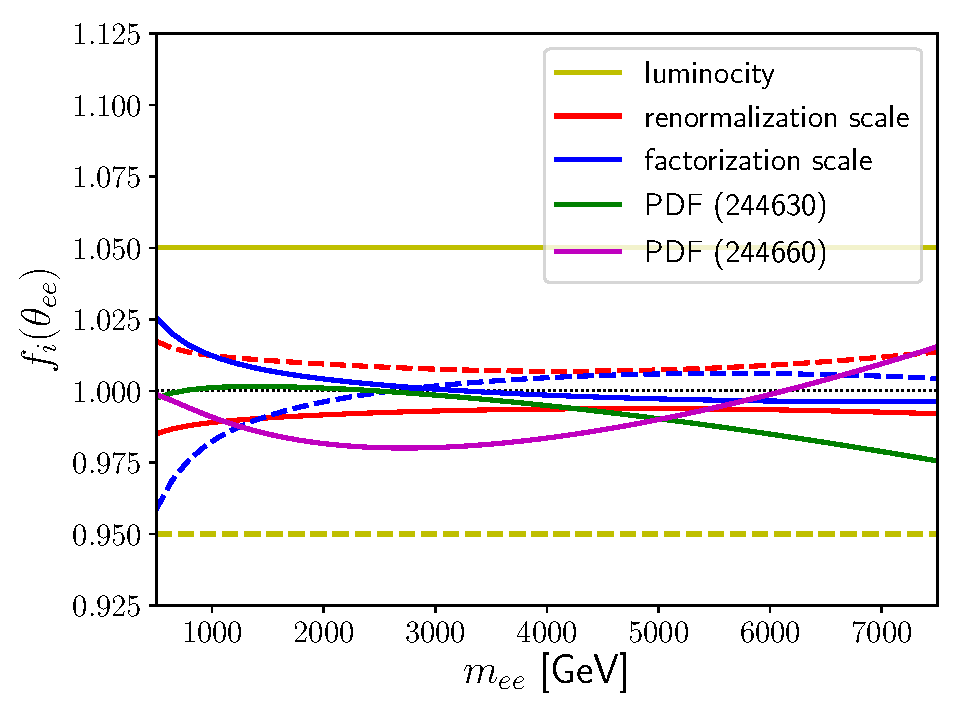
\includegraphics[width=0.5\hsize]{systematic.pdf}
  \caption{
    Form of the fitting function $f_{\mathrm{sys},i} (\bm{\theta}_f)$ evaluated with using the best fit values of $\bm{\theta}_f$ for several sources of systematic errors and $f=ee$.
    The yellow solid (dashed) line shows the result with luminosity error $+5\%$ ($-5\%$).
    The red and blue lines correspond to the different choices of the renormalization and the factorization scales, respectively, and the solid (dashed) line shows the result with $2Q$ ($Q/2$).
    The green and purple lines show results with different sets of the PDF, whose \texttt{LHAPDF6} IDs are given by 244630 and 244660, respectively.
  }
  \label{fig:systematic}
\end{figure}

To see how these errors mimic the WIMP signal, we show the form of $f_{\mathrm{sys},i} (\bm{\theta}_f)$ in Fig.~\ref{fig:systematic} for the best fit values of $\bm{\theta}_f$ under the existence of several sources of errors with $f=ee$ as an example.
The yellow solid (dashed) line shows the result with luminosity error $+5\%$ ($-5\%$).
The red and blue lines correspond to the different choices of the renormalization and the factorization scales, respectively, and the solid (dashed) line shows the result with $2Q$ ($Q/2$).
The green and purple lines show results with different sets of the PDF.
The main event set is generated by the PDF set with \texttt{LHAPDF6} ID 244600 and the green (purple) line shows the result of the \texttt{LHAPDF6} ID 244630 (244660) as an example.
From the figure, we can see that there are various forms of $\mathcal{O}(1)\,\%$ smooth corrections, including some smooth dip-like structures, all of which are well-fitted by the fitting function $f_{\mathrm{sys},i}(\bm{\theta_f})$.
Accordingly, as we will see below around Fig.~\ref{fig:nlo2}, a part of the WIMP effect, in particular a smooth part away from its dip, is also well-fitted by this function, which may decrease the sensitivity of our method significantly.

Several comments on other possible sources of systematic errors are in order.
Considering effects of the error on the beam energy, we could not generate events at NLO due to the lack of sufficient computational power.
Instead, we checked at LO that the corresponding values of $\bm{\sigma}$ (assuming that the uncertainty of the beam energy is $1\,\%$) are small enough, and hence we simply ignored it.
Two of the remaining sources are the pile-up effect and the underlying event, but they may be thought of as negligible since we are focusing on the very clean signal of two energetic leptons.
Another one is the effect of higher order contributions to the cross section including the electroweak loop correction from SM particles and that of background processes that are not considered in our analysis.
It is in principle possible to estimate their effects through the simulation and improve the analysis but here we just leave it as a future task.
Related to this, we note here that a smooth change of the number of events in general, possibly including the uncertainty listed above, could be absorbed by a minimization procedure using some fitting function like in Eq.~\eqref{eq_f_theta}.
On the other hand, as we will discuss below, the WIMP signal can not be fully absorbed by the fit because of the sharp bend we mentioned before.

We have also neglected the systematic errors from the detector effect.
The main errors are expected to come from the lepton identification, in which some of the leptons in any process are overlooked or identified incorrectly, resulting in the mis-reconstruction of the event topology.
Again, it is expected that the small and smooth modification of the number of events may be absorbed into the choice of nuisance parameters, if the corresponding values of $\bm{\sigma}_f$ are properly taken into account in addition to the values in Tables
\ref{tab_sys_ee} and \ref{tab_sys_ev}.
What is dangerous is the possible jerky modification that mimics the WIMP signal, which may be induced by the detector setup, the complicated detector response to leptons, and so on.
Such unwanted fake signals may be avoided by checking the consistency between the electron and muon channels.
This is because there should be the same size signals at the same lepton invariant mass in both channels for the WIMP signal, while the detector response to electrons and muons is different and such a coincidence is not expected in general.
It may also be helpful to look for similar fake signals in different processes associated with several leptons.
The similar treatment may also be useful to reduce the fake signals from the so-called look-elsewhere effect.
In principle, systematic errors from the detector and the look-elsewhere effects should be evaluated by repeating pseudo experiments many times including the detector simulation, but it requires a huge computational power and the detailed information of the detector construction and setup.
Thus, in this section, we just assume that these errors are well controlled once the real experiment will start and focus on the theoretical uncertainties listed in tables.


%%%%%%%%%%%%%%%%%%%%%%%%%%%%%%%%%%%%%%%%%%%%%%%%%%
\subsubsection{Detection reach}
\label{sec_detection}
%%%%%%%%%%%%%%%%%%%%%%%%%%%%%%%%%%%%%%%%%%%%%%%%%%

\begin{figure}[t]
  \centering
  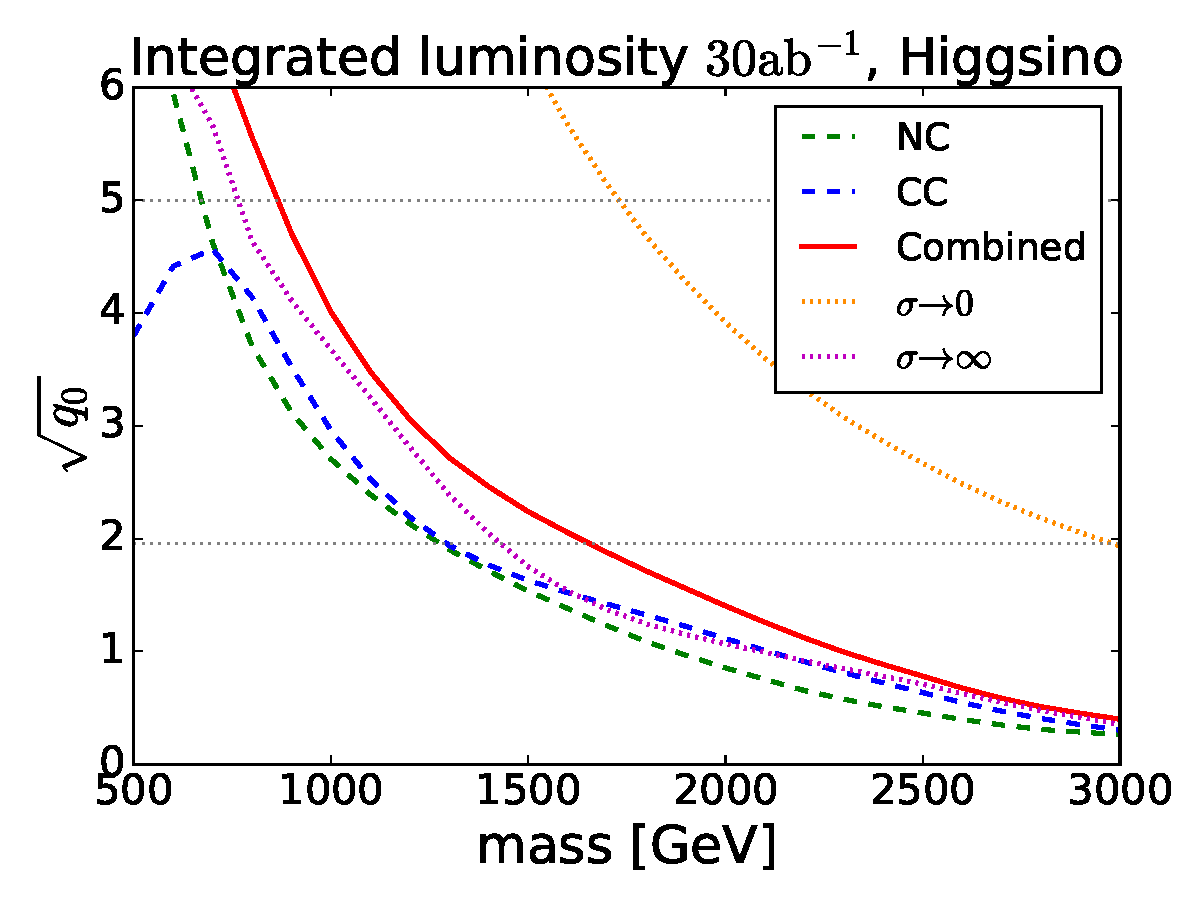
\includegraphics[width=0.48\hsize]{mchi_vs_sqq0_Higgsino.pdf}
  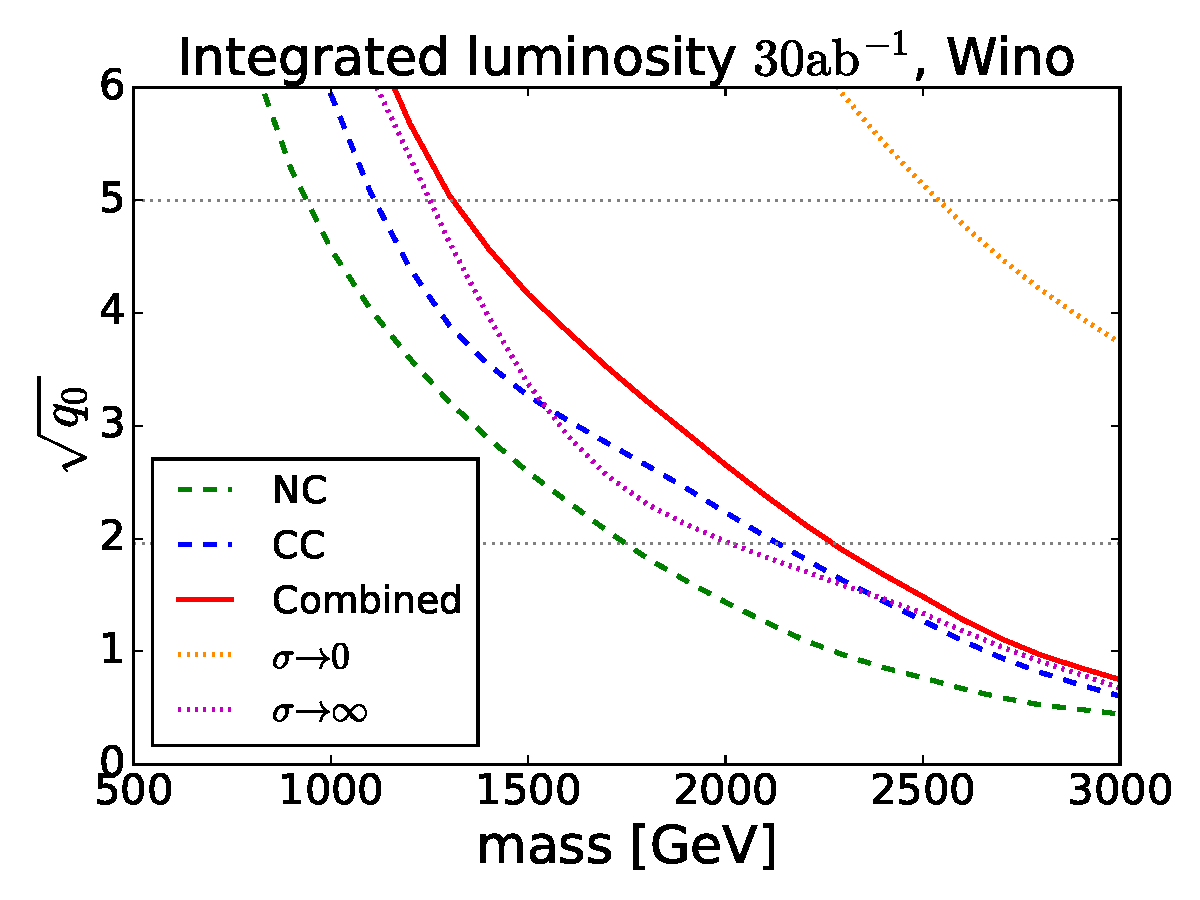
\includegraphics[width=0.48\hsize]{mchi_vs_sqq0_Wino.pdf}
  \caption{
    $\sqrt{q_0}$ as a function of the WIMP mass.
    \textbf{Left:} The figure for Higgsino.
    The green and blue dashed lines represent the results from the NC processes and the CC processes, respectively, while the red solid lines correspond to that from the combined analysis.
    The orange and purple lines denote the results from the combined analysis with the optimistic $\bm{\sigma}_f \to \bm{0}$ limit and those with conservative $\bm{\sigma}_f \to \infty$ limit, respectively.
    \textbf{Right:} The same for Wino.
  }
  \label{fig_mchi_vs_sqq0}
\end{figure}

\begin{figure}[t]
  \centering
  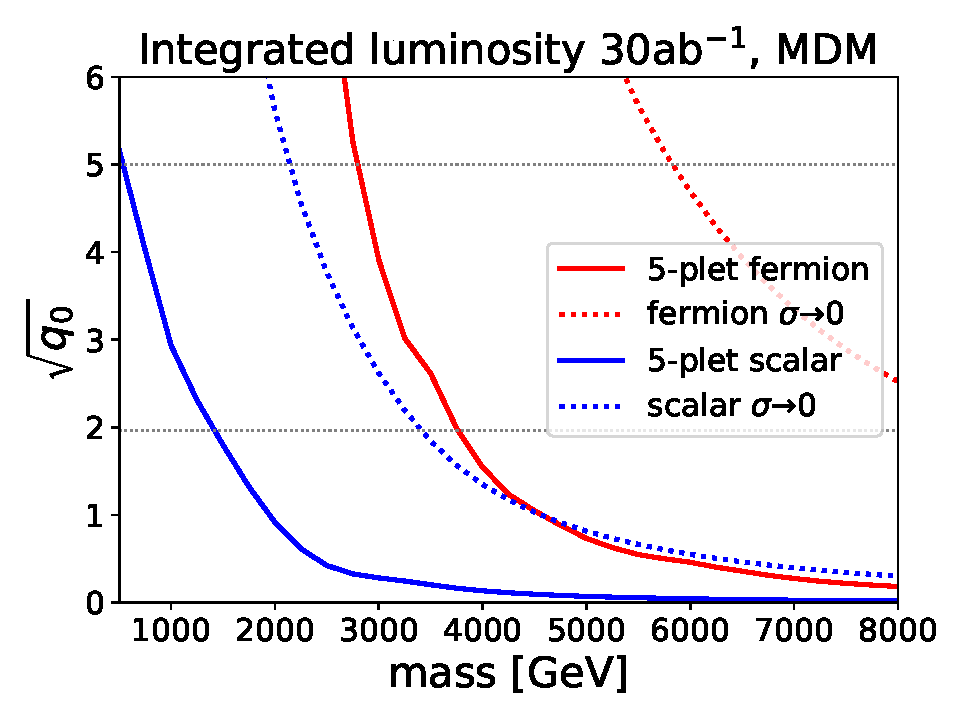
\includegraphics[width=0.48\hsize]{mchi_vs_sqq0_MDM.pdf}
  \caption{
    $\sqrt{q_0}$ as a function of the WIMP mass for the MDM models.
    The red and blue lines represent the results for 5-plet Majorana fermion and 5-plet real scalar, respectively, while the solid and dotted lines correspond to the result with and without the fitting procedure, respectively.
    All lines denote the combined results of the NC and CC processes.
  }
  \label{fig:mchi_vs_sqq0_MDM}
\end{figure}

Now we show the detection reach of WIMPs at future $100\,\mathrm{TeV}$ colliders.
In Fig.~\ref{fig_mchi_vs_sqq0}, we plot the value of $\sqrt{q_0}$ as a function of the WIMP mass, with the integrated luminosity $\mathcal{L}=30\,\mathrm{ab}^{-1}$.
As representative scenarios, we show the cases for Higgsino (the left figure) and Wino (the right figure).
In both figures, the green and blue dashed lines are the result obtained only from the NC processes and the CC processes, respectively.
We find that the CC processes are more sensitive to the effect of the WIMPs than the NC processes because of the larger cross section.
This result is consistent with Refs.~\cite{DiLuzio:2018jwd,Matsumoto:2018ioi}.
The sensitivity of the CC processes is weakened for $m \lesssim 700\, \mathrm{GeV}$ because of the lepton $p_T$ cut we have applied.\footnote
{
  We note here that the sensitivity of the CC processes depends on the lepton $p_T$ cut.
  For example, adopting the tighter cut, lepton-$p_T > 1\,\mathrm{TeV}$, the CC processes have almost no sensitivity to WIMPs with $m < 1\,\mathrm{TeV}$.
  Thus, particularly for the purpose of the Higgsino search, it is important to realize the lepton $p_T$ cut as low as $\sim 500\, \mathrm{GeV}$.
}
The combined results of the NC and CC processes are shown by the red solid lines.
By combining the two types of processes, the $5\sigma$ discovery reaches ($95\,\%$ C.L. bounds) for Higgsino and Wino are $850\,\mathrm{GeV}$ ($1.7\,\mathrm{TeV}$) and $1.3\,\mathrm{TeV}$ ($2.3\,\mathrm{TeV}$), respectively.
We find that the combination of the NC and CC processes improves the sensitivity of the WIMP mass.
Furthermore, if we understand all the systematic uncertainties quite well and effectively take the $\bm{\sigma}_f \to \bm{0}$ limit in the combined result, the detection reach will be pushed up significantly as shown by the orange dotted lines: $1.1\,\mathrm{TeV}$ Higgsino signal at well above $5\sigma$ level and a $4\sigma$ hint of the $2.9\,\mathrm{TeV}$ Wino.
These lines should be compared with the combined results and also with those obtained from the conservative analysis with $\bm{\sigma}_f \to \infty$ shown by the purple dotted lines, assuming no knowledge about sources of systematic errors.
The plot shows us that it is essential to reduce the systematic uncertainties for the detection of WIMPs through the NC and CC processes.

We also show the detection reach of the MDM scenario using both the NC and CC processes in Fig.~\ref{fig:mchi_vs_sqq0_MDM}.
The $5\sigma$ reaches are $2.8\,{\rm TeV}$ and $0.5\,{\rm TeV}$ for 5-plet fermion and 5-plet scalar, while the $95\,\%$ reaches are $3.8\,{\rm TeV}$ and $1.4\,{\rm TeV}$.
They will be improved up to $5.8\,{\rm TeV}$ and $2.2\,{\rm TeV}$ ($5\sigma$) and larger than $8\,{\rm TeV}$ and $3.4\,{\rm TeV}$ ($95\,\%$ C.L.) when the systematic errors are well understood.
If we assume the vanilla thermal freeze-out scenario, the mass should be around $10\,{\rm TeV}$ for both 5-plet fermion and scalar~\cite{Cirelli:2007xd}.
Thus, our method probes only a part of the allowed mass range for these multiplets.

\begin{figure}[t]
  \centering
  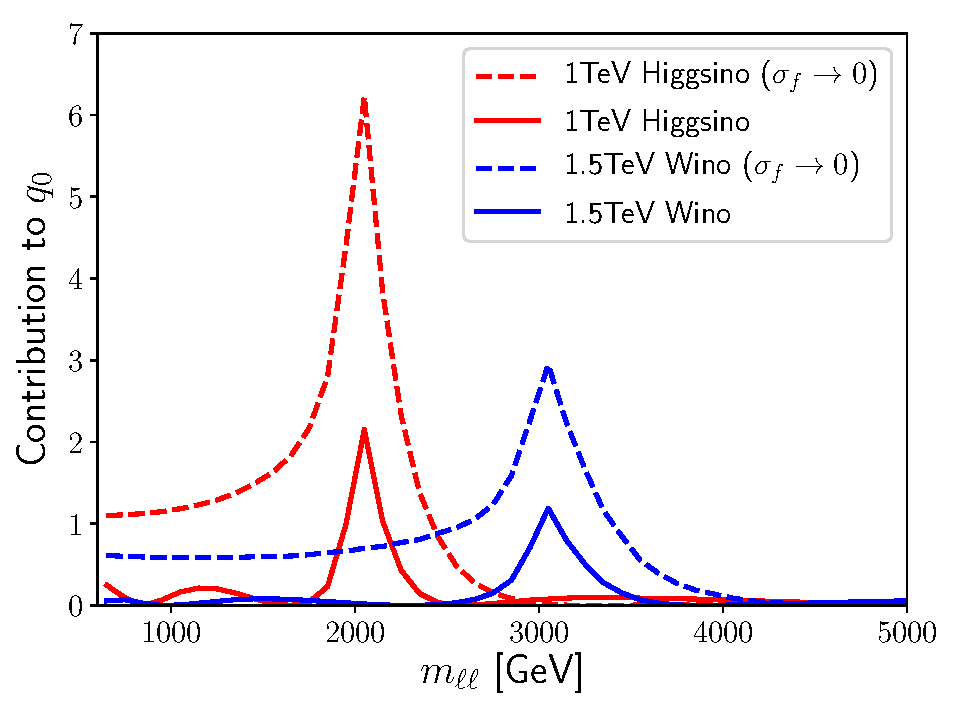
\includegraphics[width=0.495\hsize]{nlo2.pdf}
  \caption{
    Plot of the contribution of each bin to the value of $q_0$ for the NC processes.
    The red (blue) lines correspond to the $1\,\mathrm{TeV}$ Higgsino ($1.5\,\mathrm{TeV}$ Wino).
    The solid and dotted lines correspond to the results with the fitting procedure and those without it (\textit{i.e.,} the $\bm{\sigma}_f \to 0$ limit), respectively.
  }
  \label{fig:nlo2}
\end{figure}

Next, we plot in Fig.~\ref{fig:nlo2} the contribution of each bin to the value of $q_0$ to take a closer look at the significance of the dip structure, focusing on the NC processes as an example.
The red (blue) lines correspond to the $1\,\mathrm{TeV}$ Higgsino ($1.5\,\mathrm{TeV}$ Wino), while the solid and dotted lines correspond to the results with the fitting procedure and those without it (\textit{i.e.,} the $\bm{\sigma}_f \to 0$ limit), respectively.
We can see that most contributions come from the bins around the peak at $m_{\ell\ell} = 2m$.
This feature is clearer for the fitting based approach, where all the smooth parts of the correction are absorbed into the fit parameters, thus there is almost no contribution to $q_0$ from the bins other than $m_{\ell\ell} \sim 2m$.
Note also that, for the $\bm{\sigma}_f \to 0$ analysis, there are more contributions from the bins with lower $m_{\ell\ell}$ than those with higher $m_{\ell\ell}$, though sometimes the WIMP effect on the cross section is much larger in the latter bins.
This is just because of the difference in the number of events in each bin, that is $\mathcal{O}(10^7)$ for $500\,{\rm GeV} < m_{\ell\ell} < 600\,{\rm GeV}$, while $\mathcal{O}(10^3)$ for $4900\,{\rm GeV} < m_{\ell\ell} < 5000\,{\rm GeV}$ in our set up, for instance.
The similar behavior can be expected also for the CC processes.

So far, we have adopted the assumption that the distribution of the nuisance parameters is the Gaussian form and that the fitting function Eq.~\eqref{eq_f_theta} is sufficient for treating systematic errors.
In order to discuss the dependence of the results on these assumptions, we have repeated the same analysis using another distribution or fitting function.
In the former case, we have adopted the top-hat distribution: the likelihood function for the nuisance parameters $L'$ is given by
\begin{align}
  L' (\bm{\theta}_f ; \bm{\sigma}_f) \equiv \prod_\alpha
  \Theta \left( \sqrt{3}\ \sigma_{f,\alpha}
  - \left| \theta_{f,\alpha} \right| \right),
\end{align}
where $\Theta$ is the Heaviside step function.
This corresponds to the top-hat distribution of $\theta_{f,\alpha}$ with the variance $\sigma_{f,\alpha}^2$ for each $\alpha$.
As for an example of another fitting function, we have adopted a simple one-parameter extension of Eq.~\eqref{eq_f_theta}
\begin{align}
 f_{\mathrm{sys}, i} (\bm{\theta}_f) =
 e^{\theta_{f,1}} (1 - p_i)^{\theta_{f,2}}
 p_i^{(\theta_{f,3} + \theta_{f,4} \ln p_i + \theta_{f,5} \ln^2 p_i
 + \theta_{f,6} \ln^3 p_i)},\label{eq_6_param}
\end{align}
which consists of six parameters.
The variances of the nuisance parameters are estimated in the same way as Sec.~\ref{sec_statistical}, but now with the six parameters.

\begin{figure}[t]
  \centering
  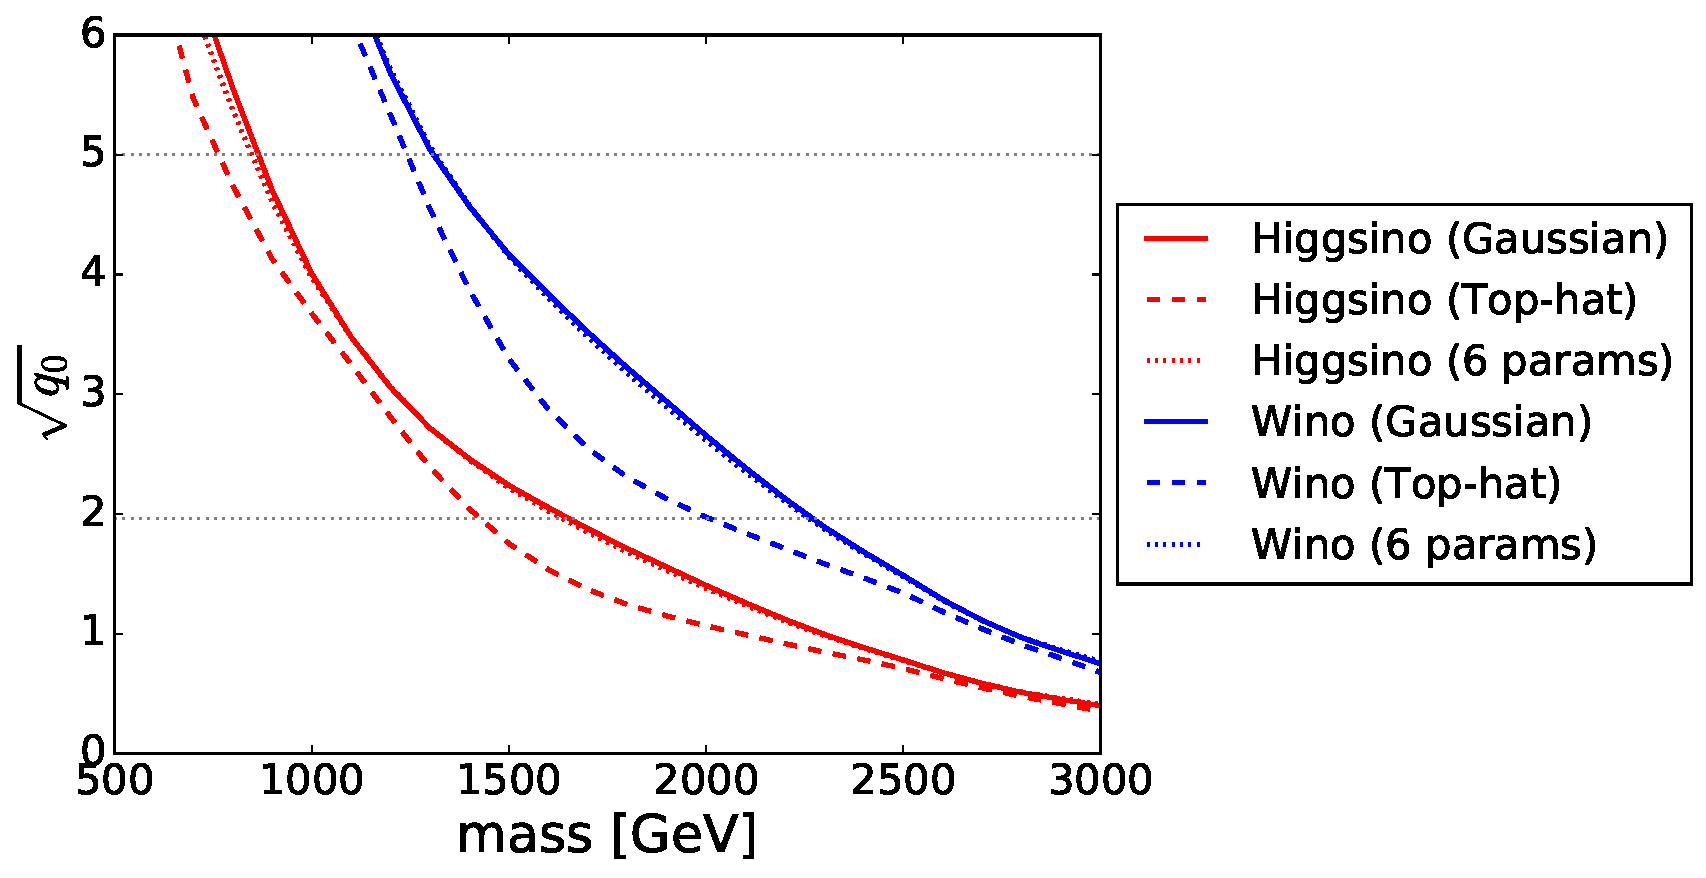
\includegraphics[width=0.7\linewidth]{mchi_vs_sqq0_comp.pdf}
  \caption{
    $\sqrt{q_0}$ as a function of the WIMP mass using both the NC and CC processes.
    The convention for the line colors is the same as Fig.~\ref{fig_mchi_vs_sqq0}.  The line styles denote the result same as Fig.~\ref{fig_mchi_vs_sqq0} (solid), that with the top-hat distribution (dashed), and that with the six parameters fitting function (dotted).
  }
  \label{fig_mchi_vs_sqq0_comp}
\end{figure}

In Fig.~\ref{fig_mchi_vs_sqq0_comp}, we show the corresponding results for Higgsino and Wino as an example.
The convention for the line colors is the same as Fig.~\ref{fig_mchi_vs_sqq0}, while the line styles denote different procedures: the dashed and dotted lines correspond to the result with the top-hat distribution and that with the six parameters fitting function, respectively, while solid lines are the same as Fig.~\ref{fig_mchi_vs_sqq0}.
From the figure, we can see that the choice of the distribution may slightly affect the result, while the addition of a nuisance parameter as Eq.~\eqref{eq_6_param} causes almost no effect.
The size of the effect of the choice of the distribution for the current estimation of errors $\bm{\sigma}_f$ is about $100\,\mathrm{GeV}$ ($200\,\mathrm{GeV}$) for the $5\sigma$ ($95\,\%$ C.L.) bounds.
We expect that such uncertainties due to the procedure to include the systematic errors will be reduced once the data from the real experiment (hence better understanding of the systematic errors) will become available.


%%%%%%%%%%%%%%%%%%%%%%%%%%%%%%%%%%%%%%%%%%%%%%%%%%
\subsubsection{Determination of WIMP properties}
\label{sec_property}
%%%%%%%%%%%%%%%%%%%%%%%%%%%%%%%%%%%%%%%%%%%%%%%%%%

In this subsection, we show that it is possible to determine the properties of the WIMPs from the NC and CC processes, thanks to the fact that we can study the $m_{\ell\ell}$ and $m_T$ distribution in great detail for these processes.
Some information about the mass, charge, and spin of the WIMPs can be extracted because the corrections to these distributions from the WIMPs are completely determined by these WIMP properties.
Firstly, we can extract the WIMP mass from the position of the dip-like structure in the correction since it corresponds to roughly twice the WIMP mass as we have shown in Sec.~\ref{sec:WIMP}.
Secondly, the overall size of the correction gives us information about the $SU(2)_L$ and $U(1)_Y$ charges.
The CC processes depend only on the $SU(2)_L$ charge, while the NC processes depend both on the $SU(2)_L$ and $U(1)_Y$ charges.
Consequently, we can obtain information about the gauge charges of the WIMPs from the NC and CC processes.

We now demonstrate the mass and charge determination of fermionic WIMPs.
This is equivalent to the determination of the parameter set $(m, C_1, C_2)$.
We generate the data assuming the SM $+$ WIMP model ($\mu=1$) with some specific values of $m, n, Y$, and $\kappa$, with which we obtain $(m, C_1, C_2)$.
We fix $\mu = 1$ for our theoretical model as well, and hence the theoretical predictions of the number of events also depend on these three parameters, $\bm{x}_f = \bm{x}_f (m, C_1, C_2)$.
We define the likelihood function $L(\check{\bm{x}}_f ; \bm{\theta}_f, m, C_1, C_2)$ in the same form as Eqs.~\eqref{eq_xtilde} and~\eqref{eq_L} with the theoretical prediction $\bm{x}_f$ now understood as a function of $(m, C_1, C_2)$, not of $\mu$.\footnote
{
  As shown in Eqs.\ \eqref{eq_C1} and \eqref{eq_C2}, $C_1$ and $C_2$ are positive quantities (and $C_2$ is discrete).
  In the figures, however, we extend the $C_1$ and $C_2$ axes down to negative regions just for presentation purposes.
}
The test statistic is defined as
%%
\begin{align}
  q (m, C_1, C_2)
  \equiv -2 \sum_f \ln \frac
  {L(\check{\bm{x}}_f ; \doublehat{\bm{\theta}}_f, m, C_1, C_2)}
  {L(\check{\bm{x}}_f ; \hat{\bm{\theta}}_f, \hat{m}, \hat{C}_1, \hat{C}_2)},
  \label{eq_q0f}
\end{align}
%%
where the parameters $(\{\hat{\bm{\theta}}_f\}, \hat{m}, \hat{C}_1, \hat{C}_2)$ maximize $\prod_f L(\check{\bm{x}}_f ; \bm{\theta}_f, m, C_1, C_2)$, while $\doublehat{\bm{\theta}}_f$ maximize
$L(\check{\bm{x}}_f ; \bm{\theta}_f, m, C_1, C_2)$ for fixed values of $(m, C_1, C_2)$.
It follows the chi-squared distribution with three degrees of freedom in the limit of a large number of events~\cite{Tanabashi:2018oca}.
The test statistic defined in this way examines the compatibility of a given WIMP model (i.e. a parameter set $(m, C_1, C_2)$) with the observed signal.


\begin{figure}[t]
  \centering
  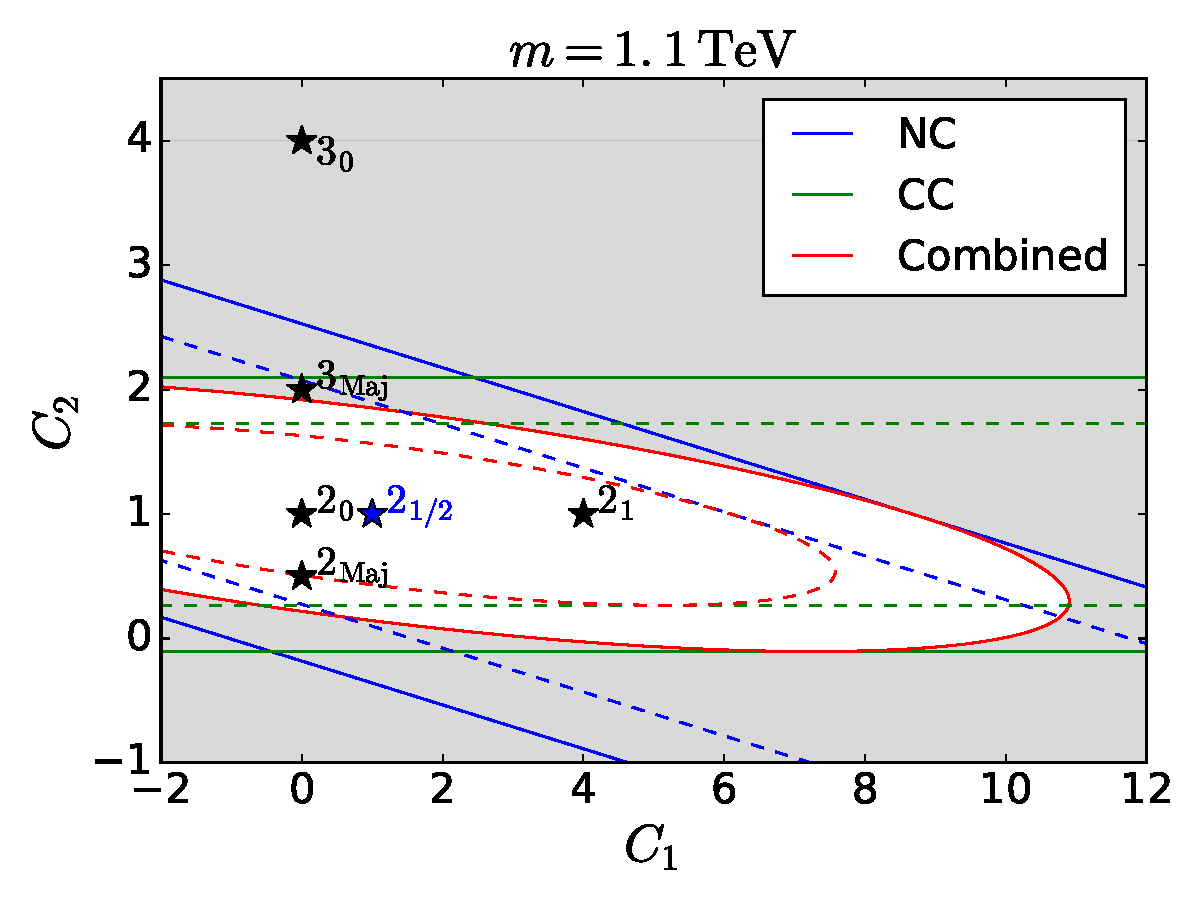
\includegraphics[width=0.5\linewidth]{C1_vs_C2_Higgsino.pdf}
  \caption{
    Contour of $\sqrt{q}$ in the $C_1~\mathrm{vs.}~C_2$ plane with $m = 1.1\,\mathrm{TeV}$, where we assume $1.1\,\mathrm{TeV}$ Higgsino signal.
    The dotted and solid lines denote $1\sigma$ and $2\sigma$ contours, respectively, and the gray region corresponds to the parameter space that is in tension with the observation at more than $2\sigma$ level.
    The blue, green, and red lines correspond to the result from the NC processes, the CC processes, and the combined analysis, respectively.
    Each star marker annotated as ``$n_Y$'' represents a point corresponding to a $SU(2)_L$ $n$-plet Dirac fermion with hypercharge $Y$, while that with ``$n_\mathrm{Maj}$'' corresponds to an $SU(2)_L$ $n$-plet Majorana fermion.
  }
  \label{fig_c1_c2}
\end{figure}

Once a deviation from the SM prediction is observed in a real experiment, we may determine $(m, C_1, C_2)$ using the above test statistic $q$.
In the following, we show the expected accuracy of the determination of $(m, C_1, C_2)$ for the case where there exists $1.1\,\mathrm{TeV}$ Higgsino.\footnote
{
  The expected significance is $3.5\sigma$ for $1.1\,\mathrm{TeV}$ Higgsino in our estimation.
  Even though it is slightly below the $5\sigma$ discovery, we take $1.1\,\mathrm{TeV}$ Higgsino as an example because it is a candidate of the thermal relic DM.
}

In Fig.~\ref{fig_c1_c2}, we show the contours of $1\sigma$ (dotted) and $2\sigma$ (solid) constraints, which correspond to the values $\sqrt{q}=1.9$ and $\sqrt{q}=2.8$, respectively, in the $C_1~\mathrm{vs.}~C_2$ plane for $m=1.1\,\mathrm{TeV}$.
The blue, green, and red lines denote the result obtained from the NC processes, the CC processes, and the combined analysis, respectively.
The models in the gray region are in more than $2\sigma$ tension with the observation.
We also show several star markers that correspond to the single $SU(2)_L$ multiplet contributions: the markers with ``$n_Y$'' represent an $SU(2)_L$ $n$-plet Dirac fermion with hypercharge $Y$, while those with ``$n_\mathrm{Maj}$'' an $SU(2)_L$ $n$-plet Majorana fermion.
Among them, the blue one with ``$2_{1/2}$'' corresponds to the Higgsino and to the best fit values in our analysis.
Both the NC and CC constraints are represented as straight bands in the $C_1~\mathrm{vs.}~C_2$ plane since each process depends on a specific linear combination of $C_1$ and $C_2$.
In particular, the CC constraint is independent of $C_1$, or $Y$.
In this sense, the NC and CC processes are complementary to each other, and thus we can separately constrain $C_1$ and $C_2$ only after combining these two results.
For instance, we can exclude a single fermionic $SU(2)_L$ multiplet with $n \neq 2$ at more than $2\sigma$ level, although each process by itself cannot exclude the possibility of $3_{\text{Maj}}$.
We can also constrain the hypercharge, yet it is not uniquely determined.
In addition to the Higgsino, the WIMP as an $SU(2)_L$ doublet Dirac fermion with $|Y|^2\lesssim 2$ or an $SU(2)_L$ doublet Majorana fermion with $|Y|^2\lesssim 5$ is still allowed.

\begin{figure}[t]
  \centering
  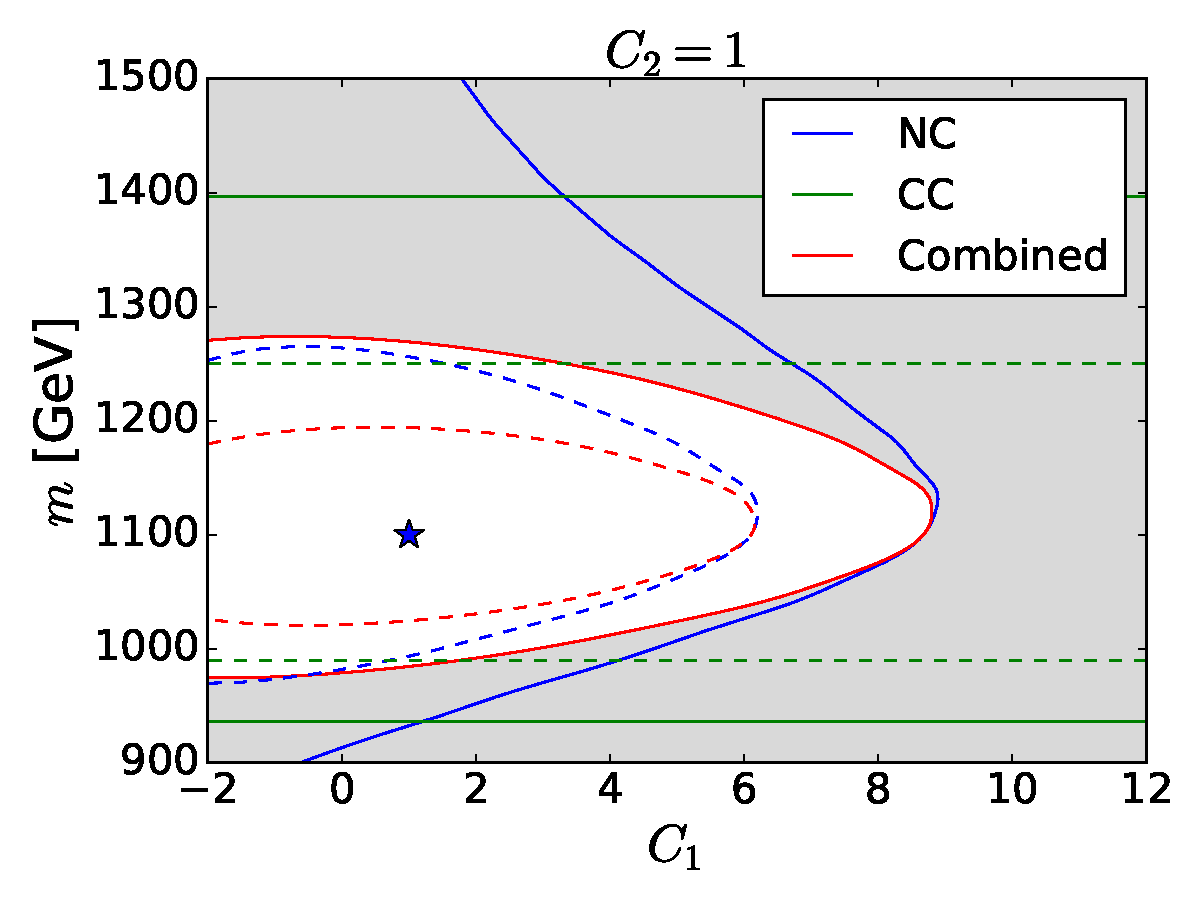
\includegraphics[width=0.48\linewidth]{C1_vs_mass_Higgsino.pdf}
  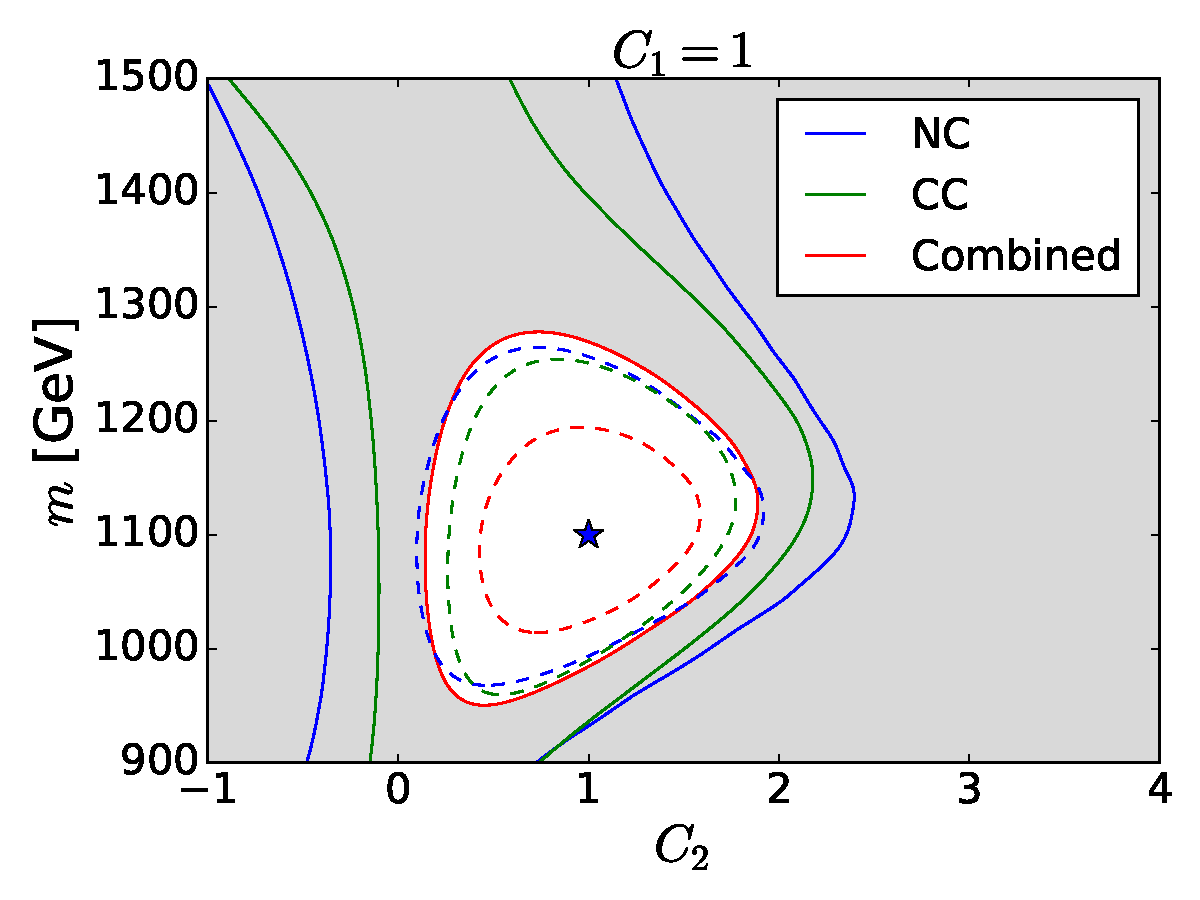
\includegraphics[width=0.48\linewidth]{C2_vs_mass_Higgsino.pdf}
  \caption{
    \textbf{Left:} Contour of $\sqrt{q}$ in the $C_1~\mathrm{vs.}~m$ plane with $C_2 = 1$, where we assume the $1.1\,\mathrm{TeV}$ Higgsino signal.
    The colors and styles of lines and the meaning of the gray region are the same as Fig.~\ref{fig_c1_c2}.
    The star maker corresponds to the true Higgsino property $(C_1, m) = (1, 1.1\,\mathrm{TeV})$.
    \textbf{Right:} Contour of $\sqrt{q}$ in the $C_2~\mathrm{vs.}~m$ plane for $C_1 = 1$, where we assume the $1.1\,\mathrm{TeV}$ Higgsino signal.
    The star maker corresponds to the true Higgsino property $(C_2, m) = (1, 1.1\,\mathrm{TeV})$.
 }
 \label{fig_c1_m}
\end{figure}

In Fig.~\ref{fig_c1_m}, we show the contour plots of $\sqrt{q}$ in the $C_1~\mathrm{vs.}~m$ plane with $C_2=1$ (left) and those in the $C_2~\mathrm{vs.}~m$ plane with $C_1=1$ (right).
The star marker in each panel shows the true values of parameters $(C_1, m) = (1, 1.1\,\mathrm{TeV})$ (left) and $(C_2, m) = (1, 1.1\,\mathrm{TeV})$ (right).
Again, by combining the NC and CC results, we can significantly improve the determination of WIMP properties, making $1\sigma$ and $2\sigma$ contours closed circles in the planes of our concern.
In particular, as red lines show, the combined analysis allows us to determine the observed WIMP mass at the level of $\mathcal{O}(10)\%$.

\begin{figure}[t]
  \centering
  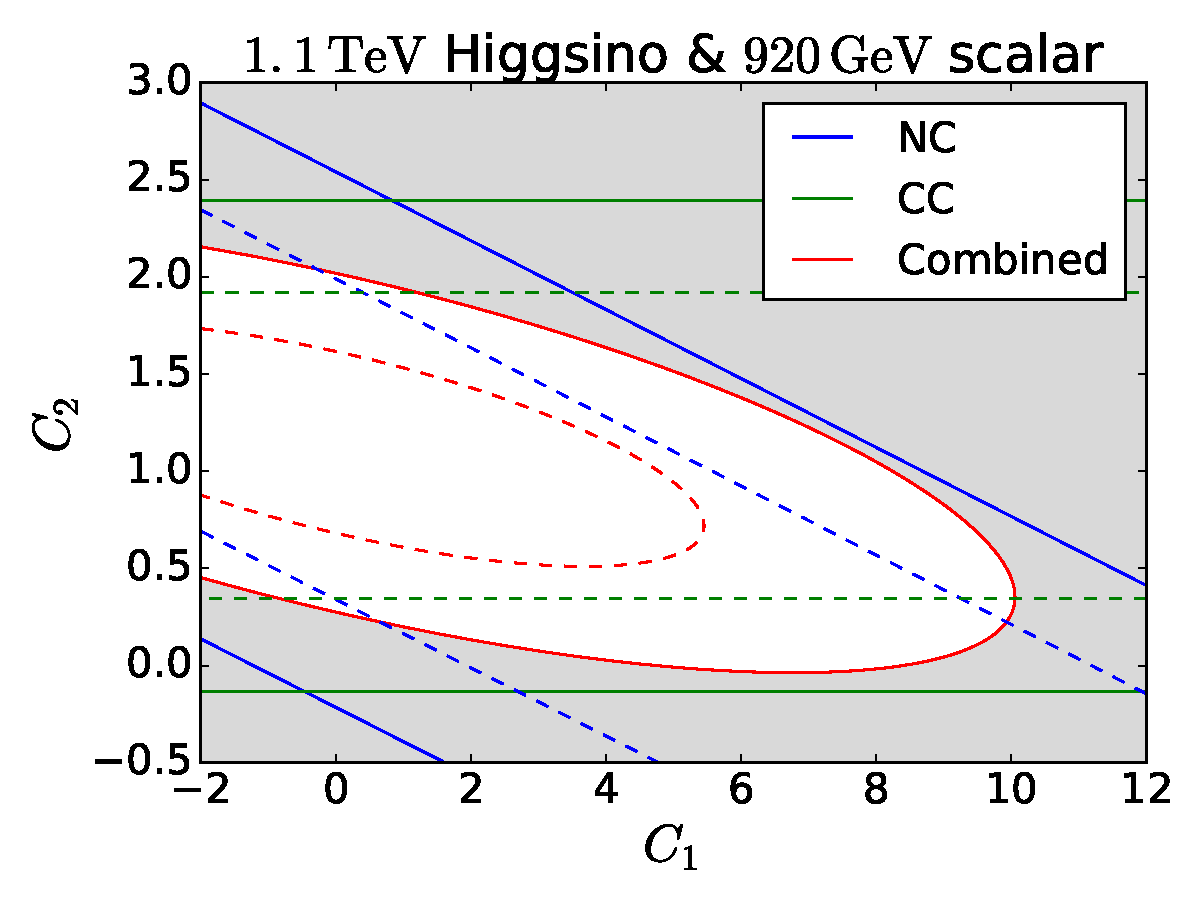
\includegraphics[width=0.5\linewidth]{C1_vs_C2_Higgsino_scalar.pdf}
  \caption{
    Contour of $\sqrt{q}$ in the $C_1~\mathrm{vs.}~C_2$ plane for the $1.1\,\mathrm{TeV}$ Higgsino signal, tested with the scalar WIMP assumption.
    The plane is defined as the scalar mass of $920\,\mathrm{GeV}$.
    The colors and styles of lines and the meaning of the gray region are the same as Fig.~\ref{fig_c1_c2}.
  }
  \label{fig_c1_c2_scalar}
\end{figure}

\begin{figure}[t]
  \centering
  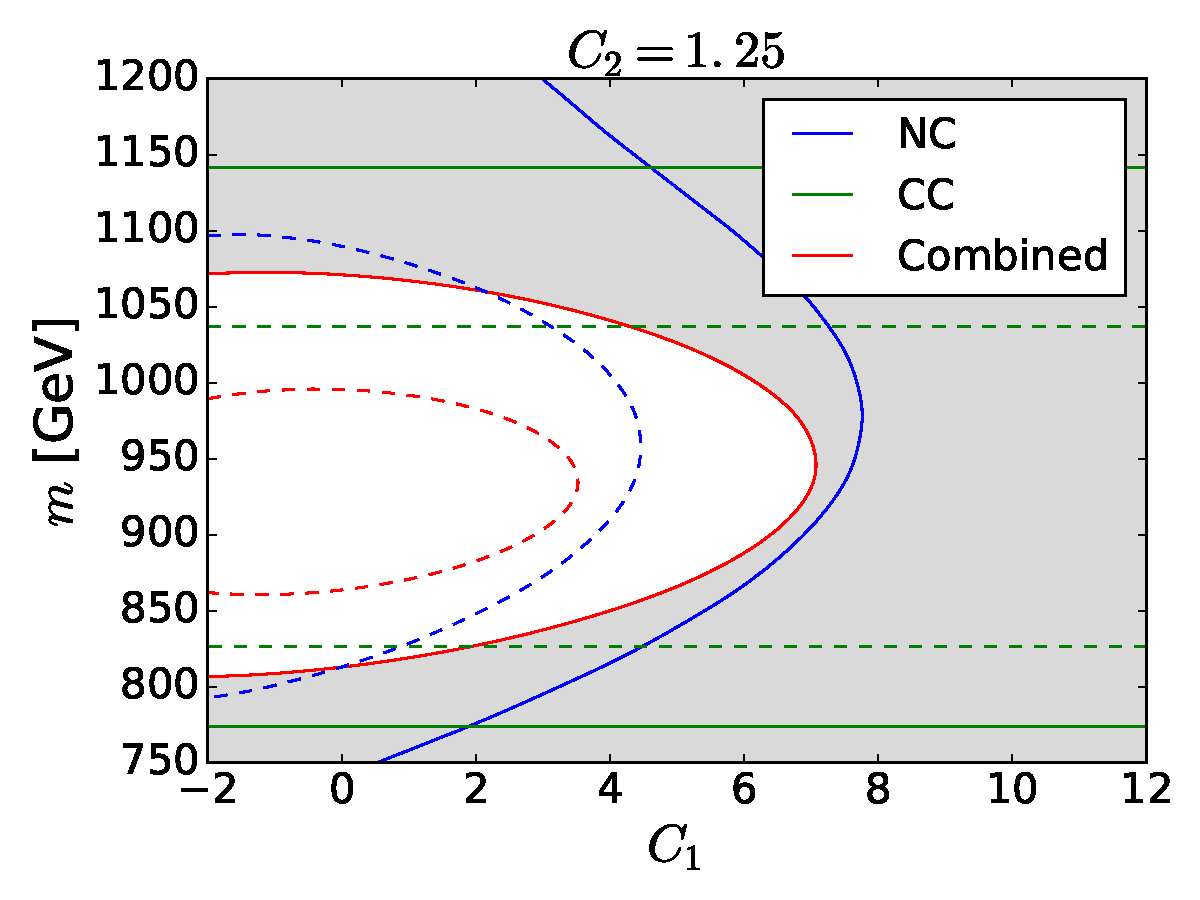
\includegraphics[width=0.48\linewidth]{C1_vs_mass_Higgsino_scalar.pdf}
  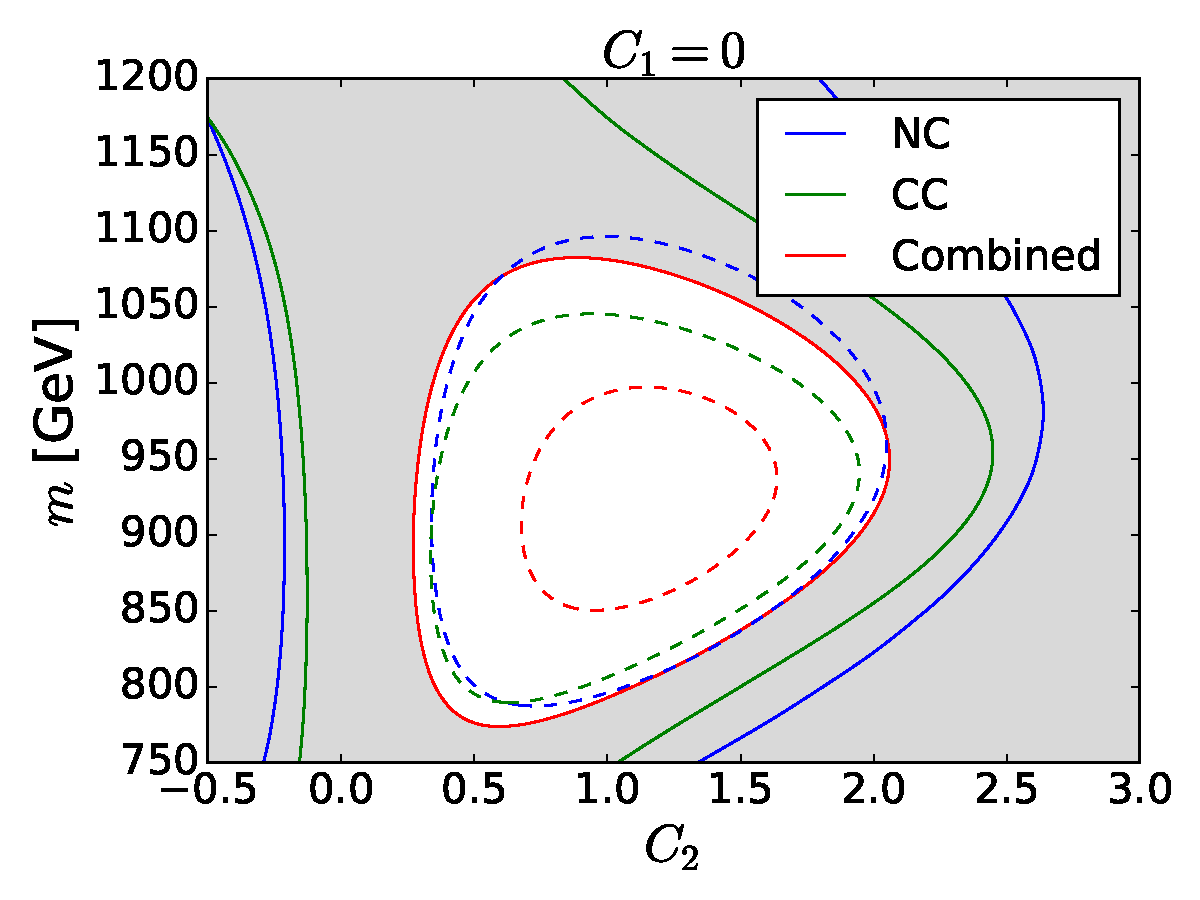
\includegraphics[width=0.48\linewidth]{C2_vs_mass_Higgsino_scalar.pdf}
  \caption{
    \textbf{Left:} Contour of $\sqrt{q}$ in the $C_1~\mathrm{vs.}~m$ plane with $C_2 = 1.25$ for the $1.1\,\mathrm{TeV}$ Higgsino signal, tested with the scalar WIMP assumption.
    The colors and styles of lines and the meaning of the gray region are the same as Fig.~\ref{fig_c1_c2}.
    \textbf{Right:} Contour  of $\sqrt{q}$ in the $C_2~\mathrm{vs.}~m$ plane with $C_1 = 0$ for the $1.1\,\mathrm{TeV}$ Higgsino signal, tested with the scalar WIMP assumption.
  }
  \label{fig_c1_m_scalar}
\end{figure}

Finally, we comment on the possibility of discriminating between fermionic and scalar WIMPs, whose difference comes from the loop function $f(x)$ (see Eq.~\eqref{eq_f}).
Here we repeat the same analysis explained above, assuming the $1.1\,\mathrm{TeV}$ Higgsino signal for example, but use the scalar loop function to evaluate the theoretical predictions $\bm{x}_f (m, C_1, C_2)$.
In Figs.~\ref{fig_c1_c2_scalar} and \ref{fig_c1_m_scalar}, we show the results in the $C_1$ vs. $C_2$ plane and the $C_1$ (or $C_2$) vs. $m$ plane, respectively, where one of the three parameters is fixed to its best fit value.
It is seen that, in the case of the $1.1\,\mathrm{TeV}$ Higgsino signal, it is hard to distinguish between the bosonic and fermionic WIMPs only with our method.
However, if a part of the WIMP properties (in particular its mass) is determined from another approach, our method may allow us to determine its spin correctly.

We also stress here that, with some favorable assumption about the observed signal, we may obtain some hint about its spin.
For example, if we assume that the observed signal composes a fraction of the dark matter in our Universe, the choice of the WIMP charges is significantly constrained.
Note from Fig.~\ref{fig_c1_c2_scalar} that the only choices of WIMP charges that allow the WIMP multiplet to contain an electrically neutral component are $(n,|Y|)=(3,0),(3,1),(4,1/2),(4,3/2)$, and $(5,0)_\text{real}$.
The last column of the table~\ref{tab:minimalDM-for-950scalar-section} shows proper choices of WIMP masses in order for their thermal relic abundances to become comparable with the dark matter abundance in the current Universe.
All of those values are somewhat larger than the central value of the mass of the observed signal, which means that the scalar interpretation of the signal cannot explain the whole of the dark matter relic abundance without introducing some non-thermal production mechanism.

\begin{table}[t]
  \centering
  \begin{tabular}{|c|ccc|}
    \hline
    $(n, Y)$           & $C_1$ & $C_2$ & $m_\text{DM}$[TeV] \\ \hline\hline
    $(3,0)_\text{real}$  &    0  &  0.25  & 2.5 \cite{Farina:2013mla}             \\
    $(3,          0)$  &    0  & 0.5   & 1.55 \cite{DelNobile:2015bqo}              \\
    $(3,          1)$  & 0.75  & 0.5   & 1.6 \cite{Farina:2013mla}               \\
    $(4,\frac{1}{2})$  & 0.25  & 1.25  & 2.4 \cite{Farina:2013mla}             \\
    $(4,\frac{3}{2})$  & 2.25  & 1.25  & 2.9 \cite{Farina:2013mla}             \\
    $(5,0)_\text{real}$  &    0  &  1.25  & 9.4 \cite{Farina:2013mla}          \\
    \hline
  \end{tabular}
  \caption{
    The scalar WIMPs that are compatible with the result in Fig.~\ref{fig_c1_c2_scalar}. The observed DM energy density is explained by the thermal relic of the WIMP with $m_{\text{DM}}$ shown in the fourth column.
  }
  \label{tab:minimalDM-for-950scalar-section}
\end{table}


%%%%%%%%%%%%%%%%%%%%%%%%%%%%%%%%%%%%%%%%%%%%%%%%%%
\subsection{Conclusion}
\label{seq:conclusion}
%%%%%%%%%%%%%%%%%%%%%%%%%%%%%%%%%%%%%%%%%%%%%%%%%%

In this section, we have discussed the indirect search of WIMPs at future $100\,\mathrm{TeV}$ hadron colliders based on the precision measurement of the production processes of a charged lepton pair and that of a charged lepton and a neutrino.
In particular, we have demonstrated that not only we can discover the WIMPs, but also we can determine their properties such as their masses, $SU(2)_L$ and $U(1)_Y$ charges, and  spins via the processes of our concern.
It is based on two facts: the high energy lepton production channel enables us to study its momentum distribution in great detail, and the WIMP correction shows characteristic features, including a dip-like structure as the final state invariant mass being twice the WIMP mass.
The latter feature also helps us to distinguish the WIMP signals from backgrounds and systematic errors, as they are not expected to show a dip-like structure.
In order to fully exploit the differences between the distributions of the WIMP signals and systematic errors, we have adopted the profile likelihood method as our statistical treatment.

First, we have shown in Fig.~\ref{fig_mchi_vs_sqq0} the detection reach of WIMPs from the NC processes (mediated by photon or $Z$-boson), the CC processes (mediated by $W$-boson), and the combination of these two results.
We have seen that the addition of the CC processes improves the detection reach from the previous analysis \cite{Chigusa:2018vxz}.
From the combined analysis, the bounds at the $5\sigma$ ($95\%$ C.L.) level for Higgsino and Wino are $850\,\mathrm{GeV}$ ($1.7\,\mathrm{TeV}$) and $1.3\,\mathrm{TeV}$ ($2.3\,\mathrm{TeV}$), respectively.
We have also shown the $5\sigma$ reach for 5-plet fermion and 5-plet scalar: $5.8\,{\rm TeV}$ and $2.2\,{\rm TeV}$ for the optimistic analysis and $2.8\,{\rm TeV}$ and $0.5\,{\rm TeV}$ for the analysis with a fitting procedure.
This result, particularly that for short lifetime Higgsino, indicates the importance of our method for the WIMP search.

Next, we have considered the determination of the mass and $SU(2)_L$ and $U(1)_Y$ charges of the observed WIMP.
By combining the NC and the CC events, the position and the height of the dip in the WIMP effect on the cross section gives us enough information for determining all the three parameters.
In Figs.~\ref{fig_c1_c2} and \ref{fig_c1_m}, we have shown the plots of the test statistics that test the validity of several choices of parameters.
As a result, the $SU(2)_L$ charge of the observed signal is correctly identified under the assumption of a single WIMP multiplet, and the $U(1)_Y$ charge and mass are also determined precisely.
In order for the determination of the WIMP spin, we have plotted the contours of the test statistics that test the validity of the scalar WIMP models with some fixed values of masses and charges.
The results are shown in Figs.~\ref{fig_c1_c2_scalar} and \ref{fig_c1_m_scalar}, which reveals that the spin is not completely determined by solely using our method.
Use of another approach to determine the WIMP properties, or of some assumption like that the observed signal corresponds to the dark matter in our Universe, may help us to obtain further information regarding the WIMP spin.

% \bibliographystyle{elsarticle-num}
% \bibliography{../phd}

\end{document}


\clearpage

\begin{appendices}

% Erase biblio in input file before turning on
\documentclass[12pt,twoside,book]{article}

\input{../settings}

\begin{document}

%%%%%%%%%%%%%%%%%%%%%%%%%%%%%%%%%%%%%%%%%%%%%%%%%%%%%%%%%%%%%%%%%%%%%%%%%%%%%%%
\section{Review of supersymmetric gauge theory}
\label{sec:susy}
%%%%%%%%%%%%%%%%%%%%%%%%%%%%%%%%%%%%%%%%%%%%%%%%%%%%%%%%%%%%%%%%%%%%%%%%%%%%%%%

\vskip 0.1in

In this appendix, we briefly review the $\mathcal{N}=1$ supersymmetric gauge theory, which is an essential element of the MSSM explained in Sec.~\ref{sec:MSSM}.
Our argument is based on~\cite{Wess:320631, Martin:1997ns}.

First, we show the $\mathcal{N} = 1$ supersymmetry algebra: \cite{Haag:1974qh}
\begin{align}
  \{ Q_\alpha, \bar{Q}_{\dot{\beta}} \} &= 2 \sigma_{\alpha
  \dot{\beta}}^\mu P_\mu,\label{QQbar} \\
  \{ Q_\alpha, Q_\beta \} &= \{ \bar{Q}_{\dot{\alpha}}
  \bar{Q}_{\dot{\beta}} \}  = 0,\label{QQQbarQbar} \\
  [ P_\mu, Q_\alpha ] &= [ P_\mu, \bar{Q}_{\dot{\alpha}} ] =
  0,\label{PQPQbar}\\
  [ P_\mu, P_\nu ] &= 0,\label{PP}
\end{align}
where $\sigma^\mu$ is defined with a unit matrix and Pauli matrices as $\sigma^\mu = (-\textbf{1},\vec{\sigma})$ and $Q_\alpha$, $\bar{Q}_{\dot{\alpha}}$, and $P_\mu$ are generators of two types of supersymmetry and translation, respectively.
Indices $(\alpha,\beta,\dot{\alpha},\dot{\beta})$ run from one to two and denote two-component Weyl spinors.
Indices $(\mu,\nu)$ run from zero to three and denotes the Lorentz four-vector.
Generators in the above algebra generates the maximally possible symmetries of the $S$-matrix including fermionic operators $Q_\alpha$ and $\bar{Q}_{\dot{\alpha}}$ by loosening the assumption on the symmetry in the derivation of the Coleman-Mandula theorem \cite{Coleman:1967ad}.

There are two important features in the representation of the supersymmetry algebra.
(I) All particles in each representation have the same mass.
(II) Bosonic and fermionic degrees of freedom in each representation are the same.
The property (I) is the direct result of the commutation relation Eq.\ (\ref{PQPQbar}).
To prove (II), we define a fermion number operator $N_F$ which has an eigenvalue $0$ for bosonic states and $+1$ for fermionic states.
From this definition, it is a straightforward work to derive the anti-commutation relation $\{(-1)^{N_F},Q\}=0$ and its conjugate.
Then the following calculation for some finite-dimensional representation of generators
\begin{align}
  {\rm Tr} \left[ (-1)^{N_F} \{Q_\alpha, \bar{Q}_{\dot{\beta}}\} \right]
  = {\rm Tr} \left[ \bar{Q}_{\dot{\beta}} \{ (-1)^{N_F}, Q_\alpha \} \right] = 0,
\end{align}
shows, using Eq.\ (\ref{QQbar}), that
\begin{align}
  2{\rm Tr} \left[ (-1)^{N_F} P_{\alpha \dot{\beta}} \right]
  = 2P_{\alpha \dot{\beta}} {\rm Tr} \left[(-1)^{N_F} \right] = 0,
\end{align}
with $P_{\alpha \dot{\beta}} \equiv \sigma^\mu_{\alpha \dot{\beta}} P_\mu$.
The first equality follows from the fact that the four momentum is universal for elements of an irreducible representation.
The last equality is just another expression of the property (II) for some non-zero four-momentum $P_{\alpha \dot{\beta}}$.

To formulate the supersymmetric field theory, it is convenient to consider the superfield, which lives on the extension of the Minkowski space with four fermionic coordinates $\theta^\alpha$ and $\bar{\theta}_{\dot{\alpha}}$, the so-called super-Minkowski space.
In a representation that acts on the super-Minkowski space, a group element corresponding to operators shown above is expressed as
\begin{align}
 G(x,\theta,\bar{\theta}) = \exp \left[ i \left( -x^\mu P_\mu + \theta Q + \bar{\theta} \bar{Q} \right) \right],
\end{align}
where the indices of fermionic objects are contracted.
Then, by calculating the product of two group elements, supersymmetry transformation is found to be a translation in the super-Minkowski space \cite{Salam:1981xd, Ferrara:1974ac}, expressed as
\begin{align}
  Q_\alpha &= \frac{\partial}{\partial \theta^\alpha} - i\sigma_{\alpha
  \dot{\alpha}}^\mu \bar{\theta}^{\dot{\alpha}} \partial_\mu,\label{Qrep} \\
  \bar{Q}^{\dot{\alpha}} &= \frac{\partial}{\partial \bar{\theta}_{\dot{\alpha}}}
  + i\theta^\alpha \sigma_{\alpha\dot{\beta}}^\mu \epsilon^{\dot{\beta} \dot{\alpha}}
  \partial_\mu.
\end{align}
It is a straightforward task to check these representations satisfy the correct commutation relations with the definition of $P_\mu \equiv -i\partial_\mu$.
In the super-Minkowski space, we can decompose the most general function as
\begin{align}
  F(x,\theta,\bar{\theta}) &= \phi(x) + \theta \psi(x) + \bar{\theta} \bar{\psi}(x)
  \notag \\
  &\quad + \theta\theta F(x) + \bar{\theta}\bar{\theta} \bar{F}(x)
  + \theta \sigma^\mu \bar{\theta} v_\mu (x) \notag \\
  &\quad + \theta\theta\bar{\theta} \lambda(x) + \bar{\theta}\bar{\theta}\theta \bar{\lambda}(x) + \theta\theta\bar{\theta}\bar{\theta} D(x),
\end{align}
where all the coefficients are general fields with proper spins under the Lorentz symmetry.
Operators involved in the supersymmetry algebra, $Q,\bar{Q}$, and $P$, naturally act on the superfield $F(x,\theta,\bar{\theta})$ with above representations.

Next we impose some constraint on the above superfield to get special superfields which possess required properties when we consider the supersymmetric extension of the SM.
First, we define chiral covariant derivatives as
\begin{align}
  D_\alpha &= \frac{\partial}{\partial \theta^\alpha} -
  2i\sigma^\mu_{\alpha \dot{\alpha}} \bar{\theta}^{\dot{\alpha}}
  \frac{\partial}{\partial y^\mu}, \\
  \bar{D}_{\dot{\alpha}} &= - \frac{\partial}{\partial \bar{\theta}^{\dot{\alpha}}},
\end{align}
where $y^\mu$ is a redefined bosonic coordinate related to $x^\mu$ as
\begin{align}
  y^\mu \equiv x^\mu + i\bar{\theta} \sigma^\mu \theta.
\end{align}
These derivatives are covariant in the meaning that they satisfy the relations
\begin{align}
  \{ Q_\alpha, D_\beta \} = \{ \bar{Q}_{\dot{\alpha}}, D_\beta \} = \{
  Q_\alpha, \bar{D}_{\dot{\beta}} \} = \{ \bar{Q}_{\dot{\alpha}},
  \bar{D}_{\dot{\beta}} \} = 0,
\end{align}
and also the following equations
\begin{align}
  (\xi Q + \bar{\xi} \bar{Q}) (D_\beta F(y,\theta,\bar{\theta})) &=
  D_\beta ((\xi Q + \bar{\xi} \bar{Q}) F(y,\theta,\bar{\theta})), \\
  (\xi Q + \bar{\xi} \bar{Q}) (\bar{D}_{\dot{\beta}}
  F(y,\theta,\bar{\theta})) &= \bar{D}_{\dot{\beta}} ((\xi Q +
  \bar{\xi} \bar{Q}) F(y,\theta,\bar{\theta})),
\end{align}
where $\xi$ and $\bar{\xi}$ are fermionic transformation parameters of the supersymmetry.
Using these derivatives, we define a chiral superfield $\Phi$ with a constraint
\begin{align}
  \bar{D}_{\dot{\alpha}} \Phi = 0,
\end{align}
or expressed explicitly in terms of component fields,
\begin{align}
  \Phi(x,\theta) &=  \phi(x) + i\theta \sigma^\mu \bar{\theta} \partial_\mu \phi(x) +
  \frac{1}{4} \theta\theta\bar{\theta}\bar{\theta} \Box \phi(x) \notag \\
  &\quad + \sqrt{2} \theta \psi(x) - \frac{i}{\sqrt{2}} \theta\theta
  \partial_\mu \psi(x) \sigma^\mu \bar{\theta} + \theta\theta F(x),\label{chiralsuperf}
\end{align}
which naturally contains a chiral fermion $\psi$ that is an important ingredient of the SM.
Since Higgs fields are also implemented in this type of multiplet as a lowest component $\phi$, the remaining piece is the spin one gauge fields $A_\mu$.
They are implemented in vector superfields defined by a constraint
\begin{align}
  V = \bar{V},
\end{align}
or in terms of component fields,
\begin{align}
  V(x,\theta,\bar{\theta}) &= C(x) + i\theta\chi(x) -
  i\bar{\theta}\bar{\chi}(x) + \frac{i}{2}\theta\theta [M(x) + iN(x)] -
  \frac{i}{2} \bar{\theta}\bar{\theta} [M(x) - iN(x)] \notag \\
  &\quad - \theta \sigma^\mu \bar{\theta} A_\mu(x) +
  i\theta\theta\bar{\theta} \left[ \bar{\lambda}(x) +
  \frac{i}{2}\bar{\sigma}^\mu \partial_\mu \chi(x) \right] -
  i\bar{\theta}\bar{\theta}\theta \left[ \lambda(x) + \frac{i}{2}
  \sigma^\mu \partial_\mu \bar{\chi}(x) \right] \notag \\
  &\quad + \frac{1}{2} \theta\theta\bar{\theta}\bar{\theta}\left[ D(x) +
  \frac{1}{2}\Box C(x)\right], \label{vectorsuperf}
\end{align}
where $\bar{\sigma}^\mu = (-\textbf{1},-\vec{\sigma})$ and component
fields are real scalar fields, Majorana fermion fields, or gauge
fields, depending on the spin under the Lorentz symmetry.  For general
gauge theories with a gauge coupling $g$ and generators $T^a_{i j}$, we
prepare several vector superfields labeled by $a$ and use a
combination $V_{i j} = 2gT^a_{i j} V^a$.

Now we demonstrate the way to construct a lagrangian invariant under the supersymmetry transformations in terms of chiral and vector superfields.
Firstly, we focus on the $\theta\theta$ component (or the F-term) of a chiral superfield $\tilde{\Phi}$, which will be denoted as $[\Phi]_F$ below, and derive its transformation rule as
\begin{align}
  \left[ (\xi Q + \bar{\xi} \bar{Q}) \Phi \right]_F
  = i\sqrt{2} \bar{\xi} \bar{\sigma}^\mu \partial_\mu \psi.
\end{align}
Since the above expression is a total derivative if $\bar{\xi}$ is a global parameter, we can add the F-term of any chiral superfield to the lagrangian.
Similarly for the vector superfield $V$, we can check that the transformation of the $\theta\theta\bar{\theta}\bar{\theta}$ component (or the D-term), which will be denoted as $[V]_D$, is a total derivative:
\begin{align}
  \left[ (\xi Q + \bar{\xi} \bar{Q}) V \right]_D = \frac{1}{2} \xi
  \sigma^\mu \partial_\mu \left[ \bar{\lambda} + \frac{i}{2}
  \bar{\sigma}^\nu \partial_\nu \chi \right] + \frac{1}{2} \bar{\xi}
  \bar{\sigma}^\mu \partial_\mu \left[ \lambda + \frac{i}{2} \sigma^\nu
  \partial_\nu \bar{\chi}\right].
\end{align}
Thus, we can also add the D-term of any vector superfield to the lagrangian.

Using what we have learned above, we can finally construct the lagrangian of a supersymmetric gauge theory.
The first important observation is that the D-term of a vector superfield $\bar{\Phi} \Phi$ contains kinetic terms of the component scalar field $\phi$ and the chiral fermion field $\psi$.
We can be easily see that
\begin{align}
  \left[ \bar{\Phi} \Phi \right]_D \sim -\partial_\mu \phi^{*}
  \partial^\mu \phi -i \bar{\psi} \bar{\sigma}^\mu \partial_\mu \psi + \bar{F}F,
\end{align}
up to surface terms.
For vector superfields, the degrees of freedom of the gauge transformation require some consideration.
As an analogy to the non-supersymmetric gauge theory, we define gauge transformation parameters $\Lambda_{i j} \equiv T^a_{i j} \Lambda_a$ using a set of chiral superfields $\Lambda_a$.
Then the transformation rule for each superfield is written as
\begin{align}
  \Phi' &= e^{-i\Lambda} \Phi,\label{chiralsfgaugetransf} \\
  \bar{\Phi}' &= \bar{\Phi} e^{i\bar{\Lambda}},  \\
  e^{V'} &= e^{-i\bar{\Lambda}} e^V e^{i\Lambda},
  \label{vectorsfgaugetransf}
\end{align}
where we use the matrix form of $V$ and $\Lambda$ defined above.
Thanks to the gauge degrees of freedom, we can choose a particular gauge in which Eq.\ (\ref{vectorsuperf}) is significantly simplified,
\begin{align}
  V_{\mathrm{WZ}} (x,\theta,\bar{\theta}) = -\theta \sigma^\mu \bar{\theta}
  A_\mu(x) + i\theta\theta \bar{\theta} \bar{\lambda}(x) -
  i\bar{\theta} \bar{\theta} \theta \lambda(x) + \frac{1}{2}
  \theta\theta \bar{\theta} \bar{\theta} D(x),
\end{align}
where the name of the gauge, the Wess-Zumino (WZ) gauge \cite{Wess:1974jb} is represented by the subscript.
Although the gauge fixing breaks supersymmetry, we can fix one reference frame of the super-Minkowski space at first, and continue our discussion under the WZ gauge in this frame.
Next we need an analog of the field strength of the non-supersymmetric gauge theory that transforms covariantly under the gauge transformation.
The required quantity is a chiral superfield defined as
\begin{align}
  \mathcal{W}_\alpha \equiv -\frac{1}{4} \bar{D} \bar{D} (e^{-V} D_\alpha e^V),
\end{align}
where its transformation rule under the gauge symmetry is
\begin{align}
 \mathcal{W}'_\alpha = e^{-i\Lambda} \mathcal{W}_\alpha e^{i\Lambda}.
\end{align}
The F-term of the invariant combination $\mathrm{Tr}[\mathcal{W}\mathcal{W}]$ contains terms proportional to the kinetic terms of $A_\mu$ and $\lambda$ as
\begin{align}
 \left[ \mathrm{Tr}[\mathcal{W}\mathcal{W}] \right]_F = 4kg^2 \left[
 -2i\lambda^a \sigma^\mu \nabla_\mu \bar{\lambda}^a - \frac{1}{2}
 F^{a\mu\nu} F^a_{\mu\nu} + D^a D^a + \frac{i}{4} F^a_{\mu\nu}
 F^a_{\rho \sigma} \epsilon^{\mu\nu\rho\sigma} \right],\label{trwawa}
\end{align}
where $k\delta^{ab} \equiv {\rm Tr}[T^a T^b]$ and $\nabla_\mu$ and $F^a_{\mu\nu}$ are the gauge covariant derivative and the field strength, respectively.
Note that the standard interaction among a gauge boson and two fermions is naturally introduced through the covariant derivative.
For later convenience, we again decompose $\mathcal{W}_\alpha$ as
\begin{align}
 \mathcal{W}_\alpha = 2g T^a \mathcal{W}^a_\alpha,
\end{align}
with which ${\rm Tr}[\mathcal{W}\mathcal{W}]$ can be deformed as
\begin{align}
  \frac{1}{4kg} {\rm Tr}[\mathcal{W}\mathcal{W}] = \mathcal{W}^a \mathcal{W}^a.
\end{align}
Finally, we have to comment that the kinetic term of a chiral superfield can be deformed to be gauge invariant.
As is easily read off from Eqs.~\eqref{chiralsfgaugetransf}--\eqref{vectorsfgaugetransf}, the combination $\bar{\Phi} e^V \Phi$, instead of $\bar{\Phi} \Phi$, becomes gauge invariant.
This modification naturally introduces gauge interactions of $\phi$ and $\psi$ as
\begin{align}
 \left[ \bar{\Phi} e^V \Phi \right]_D &\sim -\nabla_\mu \phi^{*}
 \nabla^\mu \phi -i \bar{\psi} \bar{\sigma}^\mu \nabla_\mu \psi +
 F\bar{F} \notag \\
 &\quad -\sqrt{2} g(\phi^{*} T^a \psi) \lambda^a - \sqrt{2} g
 \bar{\lambda}^a (\bar{\psi} T^a \phi) + g(\phi^{*} T^a \phi) D^a,\label{chiralkinetic}
\end{align}
up to surface terms.

\begin{table}[t]
  \centering
  \begin{tabular}{c|ccc|cc}
    & $\phi$ & $\psi$ & $F$ & bosonic & fermionic \\ \hline
    on-shell & 2 & 2 & 0 & 2 & 2 \\
    off-shell & 2 & 4 & 2 & 4 & 4 \\
  \end{tabular} \\ \vspace{5mm}
  \begin{tabular}{c|ccc|cc}
    & $A_\mu$ & $\lambda$ & $D$ & bosonic & fermionic \\ \hline
    on-shell & 2 & 2 & 0 & 2 & 2 \\
    off-shell & 3 & 4 & 1 & 4 & 4 \\
  \end{tabular}
  \caption{
    The counting of bosonic and fermionic degrees of freedom in the chiral superfield (up) and the vector superfield (down).
    Off-shell, auxiliary fields possess non-zero degrees of freedom and keep bosonic and fermionic degrees of freedom equal in each representation.
  }
  \label{tab:counting}
\end{table}

In summary, we get the supersymmetric gauge invariant lagrangian of the form
\begin{align}
 \mathcal{L}_{\rm free} = \frac{1}{4} \left[ \int d^2 \theta\ {\rm Tr}
 [\mathcal{W}^a \mathcal{W}^a] + {\rm c.c.} \right] + \int d^2 \theta
 d^2 \bar{\theta}\ \sum_{i} \bar{\Phi}_i e^V
 \Phi_i,\label{freelagrangian}
\end{align}
where the index $i$ discriminates different chiral superfields and $\int d^2 \theta$ and $\int d^2 \theta d^2 \bar{\theta}$ are the same as $[\cdots ]_F$ and $[\cdots ]_D$, respectively, because of the Grassmann nature of the coordinates $\theta$ and $\bar{\theta}$.
In the lagrangian, component fields $F_i$ and $D^a$ involved in chiral and vector superfields, respectively, are called auxiliary fields and are needed to make the supersymmetry algebra closed off-shell, \textit{i.e.}, without using equations of motion.
This can be seen from the counting of bosonic and fermionic degrees of freedom shown in Table~\ref{tab:counting}.
However, when considering on-shell, we can use equations of motion for these fields and completely eliminate them.
Then, the physical degrees of freedom left are chiral fermions $\psi_i$ and their superpartners $\phi_i$, and gauge bosons $A_\mu^a$ and their superpartners $\lambda^a$ called gauginos.

Eq.~\eqref{freelagrangian} uniquely specifies the form of sumersymmetry and gauge invariant kinetic terms and interactions among them.
Besides, we can also add interactions among chiral superfields following the procedures described above.
The most general renormalizable interaction is
\begin{align}
 \mathcal{L}_{\rm int} &= \int d^2 \theta\ W[\Phi_i] + {\rm c.c.}, \label{ref:Fterm} \\
 W[\Phi_i] &= L^i \Phi_i + M^{ij} \Phi_i \Phi_j + y^{ijk} \Phi_i \Phi_j
 \Phi_k,
\end{align}
where $W[\Phi_i]$ is called the superpotential.
Each term in the superpotential should be a gauge invariant combination of chiral superfields.
See, for example, Sec.~\ref{sec:MSSM} for the superpotential of the minimal supersymmetric standard model (MSSM).
Adding Eq.~\eqref{ref:Fterm} to the lagrangian, there are two different origins of the sclar potential in a supersymmetric gauge theory, one from the F-term of the superpotential $W[\Phi_i]$ and the other from the D-term of the gauge invariant combination $\bar{\Phi}_i e^V \Phi$.
They are often called the F-term and D-term potentials, respectively.

% \bibliographystyle{elsarticle-num}
% \bibliography{../phd}

\end{document}


\clearpage

\documentclass[12pt,twoside,book]{article}

\input{../settings}

\begin{document}

%%%%%%%%%%%%%%%%%%%%%%%%%%%%%%%%%%%%%%%%%%%%%%%%%%%%%%%%%%%%%%%%%%%%%%%%%%%%%%%
\section{Properties of the transverse mass}
\label{sec:mT}
%%%%%%%%%%%%%%%%%%%%%%%%%%%%%%%%%%%%%%%%%%%%%%%%%%%%%%%%%%%%%%%%%%%%%%%%%%%%%%%

\vskip 0.1in

In this appendix, we summarize the properties of the transverse mass, which is used for the analysis of the mono-lepton final state in Sec.~\ref{sec:dy}.
The transverse mass is useful when there is a unique invisible particle (which we will call $I$) such as a neutrino in the final state.
As already mentioned in Sec.~\ref{sec:WIMP}, the transverse mass $m_T$ is defined event by event using the measured value of the missing transverse momentum $\Slash{E}_{T}$ as
\begin{align}
  m_T^2 \equiv 2 p_T\,\Slash{E}_T \left( 1-\cos \phi \right),
\end{align}
where $p_T$ denotes the transverse momentum of a visible final state particle (which will call $P$) and $\phi$ is the difference between the azimuth angles of visible and missing transverse momenta.
It is important that we can infer the invariant mass of particles $P$ and $I$ with $m_T$, if both $P$ and $I$ are (approximately) massless.

Let $p_P$ and $p_I$ be the four momenta of $P$ and $I$, respectively.
When there is only one invisible particle in the event, the transverse momentum of $I$ is roughly identified with $\Slash{E}_T$.
Hereafter, we assume the exact equality among them just for simplicity, which corresponds to neglect the detector errors, transverse momentum of initial partons, soft emissions that are invisible for detectors, and so on.
Then, we can write the components of four momenta as
\begin{align}
  p_P &= \left( E_P, p_T \cos\phi_P, p_T \sin\phi_P, p_{Pz} \right),\\
  p_I &= \left( E_I, \Slash{E}_T \cos\phi_I, \Slash{E}_T \sin\phi_I, p_{Iz} \right),
\end{align}
with $\phi \equiv \phi_P - \phi_I$.
Note that massless conditions are satisfied, namely $E_P^2 = p_T^2 + p_{Pz}^2$ and $E_I^2 = \Slash{E}_T^2 + p_{Iz}^2$.
We can derive a relation between $m_T$ and $m_{PI} \equiv \sqrt{(p_P + p_I)^2}$
\begin{align}
  m_T \leq m_{PI},
\end{align}
where the equation holds when
\begin{align}
  p_{Pz} \Slash{E}_T - p_T p_{Iz} = 0.
\end{align}
When the above equation roughly holds, $m_{PI} - m_T$ is proportional to $(p_{Pz} \Slash{E}_T - p_T p_{Iz})^2$.

It is more intuitive to understand the situation in the center-of-mass system (CMS), focusing on the pair production process of particles $P$ and $I$.
In this case, the transverse momentum of the event is simply given by
\begin{align}
  m_T^{\mathrm{(CMS)}} = m_{PI} \sin \theta^{(\mathrm{CMS})},
  \label{eq:mT_CMS}
\end{align}
where $\theta^{(\mathrm{CMS})}$ is the angle between the momentum of $P$ and the beamline in the CMS.
Although the definition of $m_T$ is not Lorentz invariant and generally $m_T^{\mathrm{(CMS)}} \neq m_T$, the former gives a good approximation of the latter when the two-particle system is not highly boosted.
Let us simply assume $m_T = m_T^{\mathrm{(CMS)}}$ and consider the repeated production of $P$ and $I$ with fixed $m_{PI}$.
When we postulate the uniform distribution of the production cross section against $\cos \theta^{(\mathrm{CMS})}$ for simplicity, the distribution of the transverse mass $f(m_T)$ calculated according to Eq.~\eqref{eq:mT_CMS} possesses a sharp peak at $m_T = m_{PI}$, described by
\begin{align}
  f(m_T) =\frac{m_T}{m_{PI}}
  \cos^{-1} \left[ \arcsin \left( \frac{m_T}{m_{PI}} \right) \right].
  \label{eq:fmt}
\end{align}
This peak, often called the Jacobian peak, enables us to estimate $m_{PI}$ from the distribution of $m_T$.

\begin{figure}[t]
  \centering
  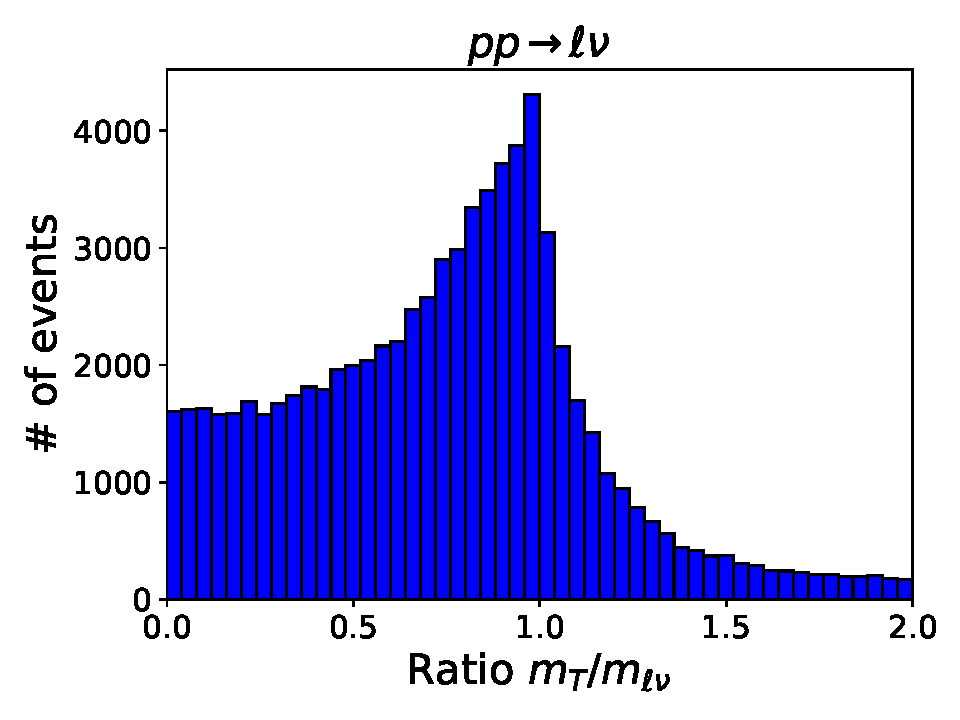
\includegraphics[width=0.5\hsize]{invariant_vs_transverse.pdf}
  \caption{
    Distribution of $m_T / m_{\ell \nu}$ for the pair production process of $P=\ell$ and $I=\nu$.
    Figure for $\sqrt{s}=100\,\mathrm{TeV}$ and $\mathcal{L}=1\,\mathrm{ab}^{-1}$.
  }
  \label{fig:invariant_vs_transverse}
\end{figure}

In Fig.~\ref{fig:invariant_vs_transverse}, we show the distribution of the ratio $m_T / m_{\ell \nu}$ for the pair production process of $P=\ell$ and $I=\nu$.
We use the setup of $\sqrt{s}=100\,\mathrm{TeV}$ and $\mathcal{L}=1\,\mathrm{ab}^{-1}$.
To evaluate the missing transverse momentum $\Slash{E}_T$ for each event, we have performed the detector simulation using \texttt{Delphes} similar to the analysis in Sec.~\ref{sec:dy}.
We can clearly see the peak at $m_T / m_{\ell \nu} = 1$, though it is somewhat smeared compared with Eq.~\eqref{eq:fmt} due to the effect of the Lorentz boost and the non-trivial angular dependence of the production cross section.
Besides, the small tail of the distribution for $m_T > m_{\ell \nu}$ can be understood as the effects we have neglected so far, such as the detector errors.

\end{document}


\clearpage

\documentclass[12pt,twoside,book]{article}

\input{../settings}

\begin{document}

%%%%%%%%%%%%%%%%%%%%%%%%%%%%%%%%%%%%%%%%%%%%%%%%%%%%%%%%%%%%%%%%%%%%%%%%%%%%%%%
\section{Profile likelihood method}
\label{sec:profile}
%%%%%%%%%%%%%%%%%%%%%%%%%%%%%%%%%%%%%%%%%%%%%%%%%%%%%%%%%%%%%%%%%%%%%%%%%%%%%%%

\vskip 0.1in

In this appendix, we briefly review the profile likelihood method used in Sec.~\ref{sec_statistical}.
In particular, we describe the motivation and justification to consider this method.

First of all, the experimental outcome can be expressed as a set of random variables $\bm{x} \equiv \{ x_1, \cdots, x_n \}$, with $n$ being the number of observables.
The distribution of these variables is due to both the intrinsic physical randomness (\textit{i.e.}, the statistical fluctuation) and the uncertainty in detector responses such as the efficiency, momentum reconstruction, and so on.
We assume $\bm{x}$ obey some probability distribution function and express it as $f(\bm{x} ; \bm{\theta})$, where $\bm{\theta} = \{ \theta_1, \cdots, \theta_m \}$ parametrize (in many cases unknown) uncertainties listed above.
When we repeat $N$ experiments and obtain $N$ sets of observables expressed as $\bm{x}^a$ ($a = 1,\cdots,N$), we define the likelihood function $L$ as
\begin{align}
  L = \prod_{a=1}^N f(\bm{x}^a ; \bm{\theta}).
\end{align}
Since $L$ should take a relatively larger value if the assumed distribution $f$ approximates the reality very well, we may perform the maximization of $L$ against the choice of $\bm{\theta}$ to obtain the correct probability distribution.
Such a maximization procedure can be performed analytically only for several simple distribution functions.
Thus, in many cases, we need a numerical calculation of the maximization procedure, which can be performed with the \texttt{MINUIT} package \cite{James:1994vla}.

In our analysis in Sec.~\ref{sec:dy}, the data is given in the form of the histogram.
In this case, $x_i$ $(i=1, \cdots, n)$ denotes the observed number of events in each bin labeled by $i$, with $n$ being the number of bins.
Then the likelihood $L$, which is the product of the probability distribution function for each bin, is expressed as
\begin{align}
  L(\bm{x} ; \bm{\theta}) \equiv \prod_i f_i(\bm{x} ; \bm{\theta}) = \prod_i \exp \left[
    - \frac{\left(x_i - \mu_i (\bm{\theta}) \right)^2}{2 x_i}
  \right],
\end{align}
with $\mu_i (\bm{\theta})$ being the average number of events of the bin $i$ calculated using the parameters $\bm{\theta}$.
Note that $x_i \gg 1$ is assumed for each bin and the central limit theorem is used to replace the Poisson to the Gaussian distribution.
Then, it is clear that the maximization of $L$ is equivalent to the minimization of $\chi^2$ defined as
\begin{align}
  \chi^2 \equiv -2 \ln L(\bm{x} ; \bm{\theta}) = \sum_{i=1}^{n}
  \frac{\left(x_i - \mu_i (\bm{\theta}) \right)^2}{x_i},
\end{align}
which is the so-called Neyman's $\chi^2$ variable.
$\chi^2$ obeys the chi-squared distribution when the distribution of $x_i$ is well approximated by the Gaussian and can be easily used to estimate the errors of $\bm{\theta}$ around the optimized values.

Similarly, one can apply the likelihood maximization to the model test.
Let $\bm{\theta}_{\mathrm{true}}$ and $\bm{\theta}_{\mathrm{test}}$ be the model in reality and that we want to test, respectively.
For example, in the new physics search, the former corresponds to a new physics model of our concern, while the latter to the SM.
Then we can define the test-statistic
\begin{align}
  q (\bm{\theta}_{\mathrm{test}}) =
  -2 \ln \frac{L(\bm{x} ; \bm{\theta}_{\mathrm{test}})}
  {L(\bm{x} ; \bm{\theta}_{\mathrm{true}})},
\end{align}
which plays the role of the so-called $\Delta \chi^2$ variable according to the discussion above.
Again $q$ may obey a chi-squared distribution with some degrees of freedom, and can be used to obtain sensitivities to the new physics, \textit{e.g.,} the $95\,\%$ C.L. exclusion and the $5\sigma$ discovery.
Note that the denominator of the test statistic can also be expressed as $L(\bm{x} ; \hat{\bm{\theta}})$, where the hat denotes the values of $\bm{\theta}$ that maximize the function $L$.

However, the situation may be more complicated since some of the parameters $\bm{\theta}$ are not directly related to the model parameters, but express the background yield, detector effects, systematic errors, and so on, which should be determined from experimental data.
Such additional parameters are often called nuisance parameters.
To treat nuisance parameters, it is convenient to rely on the profile likelihood method \cite{Cowan:2010js}.

For this purpose, we divide the parameters into two categories: the model parameter of our interest $\bm{\mu}$ and nuisance parameters $\bm{\theta}$.
Similarly to the discussion without the nuisance parameters, let $\bm{\mu}$ be the model that we want to test.
The test static is defined as
\begin{align}
  q (\bm{\mu}) =
  -2 \ln \frac{L(\bm{x} ; \bm{\mu}, \doublehat{\bm{\theta}} (\bm{\mu}))}
  {L(\bm{x} ; \hat{\bm{\mu}}, \hat{\bm{\theta}})},
\end{align}
where the meaning of the hat is the same as above, while $\doublehat{\bm{\theta}} (\bm{\mu})$ denotes the values that maximize $L$ with fixed values of $\bm{\mu}$.
The motivation for this definition is provided by the Wilk's theorem \cite{wilks1938}, which proves that $q (\bm{\mu})$ asymptotically obeys the chi-squared distribution whose degrees of freedom equal to the number of model parameters $\bm{\mu}$.
Note that this statement is highly non-trivial since the individual term $-2\ln L$ \textit{does not} obey a chi-squared distribution in this case.
Thanks to the theorem, we can perform the same analysis under the existence of nuisance parameters and, in particular, absorb the effects of systematic errors into the choice of parameters $\bm{\theta}$.

\rem{Clarify d.o.f}

\rem{Comment on distribution of nuisance parameters?}

% \bibliographystyle{elsarticle-num}
% \bibliography{../phd}

\end{document}


\end{appendices}

\clearpage

\bibliographystyle{elsarticle-num}
\bibliography{phd}

\end{document}
